
% Plantilla para un Trabajo Fin de Grado de la Universidad de Granada,
% adaptada para el Doble Grado en Ingeniería Informática y Matemáticas.
%
%  Autor original de la plantilla original: Mario Román.
%  Enlace: https://github.com/mroman42/templates
%  Cambios en la plantilla por: Javier Sáez
%  Licencia: GNU GPLv2.
%
% Esta plantilla es una adaptación al castellano de la plantilla
% classicthesis de André Miede, que puede obtenerse en:
%  https://ctan.org/tex-archive/macros/latex/contrib/classicthesis?lang=en
% La plantilla original se licencia en GNU GPLv2.
%
% Esta plantilla usa símbolos de la Universidad de Granada sujetos a la normativa
% de identidad visual corporativa, que puede encontrarse en:
% http://secretariageneral.ugr.es/pages/ivc/normativa
%
% La compilación se realiza con las siguientes instrucciones:
%   pdflatex --shell-escape main.tex
%   bibtex main
%   pdflatex --shell-escape main.tex
%   pdflatex --shell-escape main.tex

% Opciones del tipo de documento
\documentclass[oneside,openright,titlepage,numbers=noenddot,openany,headinclude,footinclude=true, cleardoublepage=empty,abstractoff,BCOR=5mm,paper=a4,fontsize=11pt, dvipsnames,table,xcdraw]{scrreprt}

% LaTeX packages loaded on start
\usepackage[utf8]{inputenc}
\usepackage[T1]{fontenc}
\usepackage{fixltx2e}
\usepackage{graphicx} % Inclusión de imágenes.
\usepackage{grffile}  % Distintos formatos para imágenes.
\usepackage{longtable} % Tablas multipágina.
\usepackage{wrapfig} % Coloca texto alrededor de una figura.
\usepackage{rotating}
\usepackage[normalem]{ulem}
\usepackage{amsmath}
\usepackage{textcomp}
\usepackage{amssymb}
\usepackage{capt-of}
\usepackage[colorlinks=true]{hyperref}
\usepackage{tikz} % Diagramas conmutativos.
\usepackage{minted} % Código fuente.
\usepackage[T1]{fontenc}
\usepackage{natbib}
\usepackage{caption}
\usepackage{ mathrsfs }



\usepackage[toc,page]{appendix}

%% ---------------------- Self added packages
\usepackage{cancel}
\usepackage{cleveref}
\usepackage{bm}
\usepackage{witharrows}
\usepackage{algorithmic}
\usepackage{ upgreek }
\usepackage{wrapfig}
\usepackage{multirow}
\usepackage{svg}


%License

% License
\usepackage[
    type={CC},
    modifier={by-sa},
    version={4.0},
]{doclicense}

%% ---------------------------------

% Plantilla classicthesis
\usepackage[beramono,eulerchapternumbers,linedheaders,parts,a4paper,dottedtoc,
manychapters,pdfspacing]{classicthesis}

% Geometría y espaciado de párrafos.
\setcounter{secnumdepth}{0}
\usepackage{enumitem}
\setitemize{noitemsep,topsep=0pt,parsep=0pt,partopsep=0pt}
\setlist[enumerate]{topsep=0pt,itemsep=-1ex,partopsep=1ex,parsep=1ex}
\usepackage[top=1in, bottom=1.5in, left=0.9in, right=1.2in]{geometry}
\setlength\itemsep{0em}
\setlength{\parindent}{0pt}
\usepackage{parskip}

% Algoritmos
\usepackage[ruled,vlined]{algorithm2e}
\newcommand\mycommfont[1]{\footnotesize\ttfamily\textcolor{blue}{#1}}
\SetCommentSty{mycommfont}

% Todo notes
\usepackage{todonotes}
\let\marginpar\oldmarginpar

% Profundidad de la tabla de contenidos.
\setcounter{secnumdepth}{3}

% Usa el paquete minted para mostrar trozos de código.
% Pueden seleccionarse el lenguaje apropiado y el estilo del código.
\usepackage{minted}
\usemintedstyle{colorful}
\setminted{fontsize=\small}
\renewcommand{\theFancyVerbLine}{\sffamily\textcolor[rgb]{0.5,0.5,1.0}{\oldstylenums{\arabic{FancyVerbLine}}}}

% Archivos de configuración.
%------------------------
% Math libraries
%------------------------
\usepackage{amsthm}
\usepackage{amsmath}
\usepackage{tikz}
\usepackage{tikz-cd}
\usetikzlibrary{shapes,fit}
\usepackage{bussproofs}
\EnableBpAbbreviations{}
\usepackage{mathtools}
\usepackage{scalerel}
\usepackage{stmaryrd}

%------------------------
% Estilos para los teoremas
%------------------------
\theoremstyle{plain}
\newtheorem{nth}{Theorem}
\newtheorem{nprop}{Proposition}
\newtheorem{lemma}{Lemma}
\newtheorem{corollary}{Corollary}
\theoremstyle{definition}
\newtheorem{ndef}{Definition}
\newtheorem{nproof}{Proof}
\theoremstyle{remark}
\newtheorem{remark}{Remark}
\newtheorem{nexample}{Example}

\begingroup\makeatletter\@for\theoremstyle:=definition,remark,plain\do{\expandafter\g@addto@macro\csname th@\theoremstyle\endcsname{\addtolength\thm@preskip\parskip}}\endgroup

%------------------------
% Macros
% ------------------------

%Frequently used mathematical commands
\newcommand*\diff{\mathop{}\!\mathrm{d}}
\newcommand{\R}{\mathbb{R}}
% \newcommand{\E}{\mathbb{E}}
\newcommand{\bmu}{\bm{\mu}}
\newcommand{\bx}{\bm{x}}
\newcommand{\bX}{\bm{X}}
\newcommand{\bz}{\bm{z}}
\newcommand{\bZ}{\bm{Z}}
\newcommand{\bv}{\bm{v}}
\newcommand{\bh}{\bm{h}}
\newcommand{\bSigma}{\bm{\Sigma}}
\newcommand{\bpi}{\bm{\pi}}
\newcommand{\bLambda}{\bm{\Lambda}}
\newcommand{\btheta}{\bm{\theta}}

\newcommand{\V}{\mathcal{V}}
\newcommand{\D}{\mathcal{D}}
\newcommand{\X}{\mathcal{X}}
\newcommand{\I}{\mathcal{I}}

\newcommand\ddfrac[2]{\frac{\displaystyle #1}{\displaystyle #2}}

\newcommand\E[2]{\mathbb{E}_{#1}\Big[#2\Big]}
\newcommand\KL[2]{KL\Big(#1 \bigm| #2\Big)}
\newcommand{\bigCI}{\mathrel{\text{\scalebox{1.07}{$\perp\mkern-10mu\perp$}}}}
\newcommand{\bigCD}{\centernot{\bigCI}}

\DeclareMathOperator*{\argmax}{arg\,max}
\DeclareMathOperator*{\argmin}{arg\,min}

% My own commands:

\newcommand{\Prob}{\mathcal{P}}
\newcommand{\Alg}{\mathscr{A}}
\newcommand{\N}{\mathbb N}
\newcommand{\A}{\mathcal A}

\newcommand{\abs}[1]{\lvert#1\rvert}  

% Math operators

\DeclareMathOperator*{\Var}{Var}

  % En macros.tex se almacenan las opciones y comandos para escribir matemáticas.
% ****************************************************************************************************
% classicthesis-config.tex 
% formerly known as loadpackages.sty, classicthesis-ldpkg.sty, and classicthesis-preamble.sty 
% Use it at the beginning of your ClassicThesis.tex, or as a LaTeX Preamble 
% in your ClassicThesis.{tex,lyx} with % ****************************************************************************************************
% classicthesis-config.tex 
% formerly known as loadpackages.sty, classicthesis-ldpkg.sty, and classicthesis-preamble.sty 
% Use it at the beginning of your ClassicThesis.tex, or as a LaTeX Preamble 
% in your ClassicThesis.{tex,lyx} with % ****************************************************************************************************
% classicthesis-config.tex 
% formerly known as loadpackages.sty, classicthesis-ldpkg.sty, and classicthesis-preamble.sty 
% Use it at the beginning of your ClassicThesis.tex, or as a LaTeX Preamble 
% in your ClassicThesis.{tex,lyx} with \input{classicthesis-config}
% ****************************************************************************************************  
% If you like the classicthesis, then I would appreciate a postcard. 
% My address can be found in the file ClassicThesis.pdf. A collection 
% of the postcards I received so far is available online at 
% http://postcards.miede.de
% ****************************************************************************************************


% ****************************************************************************************************
% 0. Set the encoding of your files. UTF-8 is the only sensible encoding nowadays. If you can't read
% äöüßáéçèê∂åëæƒÏ€ then change the encoding setting in your editor, not the line below. If your editor
% does not support utf8 use another editor!
% ****************************************************************************************************
\PassOptionsToPackage{utf8x}{inputenc}
	\usepackage{inputenc}

% ****************************************************************************************************
% 1. Configure classicthesis for your needs here, e.g., remove "drafting" below 
% in order to deactivate the time-stamp on the pages
% ****************************************************************************************************
%Old
%\PassOptionsToPackage{eulerchapternumbers,listings,drafting,%
%		pdfspacing,%floatperchapter,%linedheaders,%
%                subfig,beramono,eulermath,parts,dottedtoc}{classicthesis}                                        
% ********************************************************************
% Arsclassica , another template
\usepackage{arsclassica}
\PassOptionsToPackage{
  drafting=true,    % print version information on the bottom of the pages
  tocaligned=false, % the left column of the toc will be aligned (no indentation)
  dottedtoc=false,  % page numbers in ToC flushed right
  eulerchapternumbers=true, % use AMS Euler for chapter font (otherwise Palatino)
  linedheaders=false,       % chaper headers will have line above and beneath
  floatperchapter=true,     % numbering per chapter for all floats (i.e., Figure 1.1)
  eulermath=true,  % use awesome Euler fonts for mathematical formulae (only with pdfLaTeX)
  beramono=true,    % toggle a nice monospaced font (w/ bold)
  iosevka=true,
  palatino=true,    % deactivate standard font for loading another one, see the last section at the end of this file for suggestions
  style=arsclassica % classicthesis, arsclassica
}{classicthesis}


%\newcommand*{\Chapter}[1]{%
%
%	\chapter{}%[#1: \textit{#2}]{#1}%
%    \begingroup
%    \raggedright\Large
%    \spacedallcaps{#1}\par
%    \endgroup
%    \nobreak\vspace{\glueexpr \bigskipamount*3 \relax}%
%    % Adjust this factor as needed ..........^
%}

\renewcommand\formatchapter[1]{%
    \setbox0\hbox{\chapterNumber\thechapter\hspace{10pt}\ \\ }%
    \begin{minipage}[t]{\dimexpr\linewidth-\wd0\relax}%
    \raggedright\spacedallcaps{#1}%
    \end{minipage}%
}






% Available options for classicthesis.sty 
% (see ClassicThesis.pdf for more information):
% drafting
% parts nochapters linedheaders
% eulerchapternumbers beramono eulermath pdfspacing minionprospacing
% tocaligned dottedtoc manychapters
% listings floatperchapter subfig
% ********************************************************************

% ****************************************************************************************************
% 2. Personal data and user ad-hoc commands
% ****************************************************************************************************
\newcommand{\myTitle}{A Classic Thesis Style\xspace}
\newcommand{\mySubtitle}{An Homage to The Elements of Typographic Style\xspace}
\newcommand{\myDegree}{Doktor-Ingenieur (Dr.-Ing.)\xspace}
\newcommand{\myName}{André Miede\xspace}
\newcommand{\myProf}{Put name here\xspace}
\newcommand{\myOtherProf}{Put name here\xspace}
\newcommand{\mySupervisor}{Put name here\xspace}
\newcommand{\myFaculty}{Put data here\xspace}
\newcommand{\myDepartment}{Put data here\xspace}
\newcommand{\myUni}{Put data here\xspace}
\newcommand{\myLocation}{Saarbrücken\xspace}
\newcommand{\myTime}{September 2015\xspace}
%\newcommand{\myVersion}{version 4.2\xspace}

% ********************************************************************
% Setup, finetuning, and useful commands
% ********************************************************************
\newcounter{dummy} % necessary for correct hyperlinks (to index, bib, etc.)
\newlength{\abcd} % for ab..z string length calculation
\providecommand{\mLyX}{L\kern-.1667em\lower.25em\hbox{Y}\kern-.125emX\@}
\newcommand{\ie}{i.\,e.}
\newcommand{\Ie}{I.\,e.}
\newcommand{\eg}{e.\,g.}
\newcommand{\Eg}{E.\,g.} 
% ****************************************************************************************************


% ****************************************************************************************************
% 3. Loading some handy packages
% ****************************************************************************************************
% ******************************************************************** 
% Packages with options that might require adjustments
% ******************************************************************** 
%\PassOptionsToPackage{ngerman,american}{babel}   % change this to your language(s)
% Spanish languages need extra options in order to work with this template
% \PassOptionsToPackage{es-lcroman,spanish}{babel}
\usepackage[main=english]{babel}

%\usepackage{csquotes}
% \PassOptionsToPackage{%
%     %backend=biber, %instead of bibtex
% 	backend=bibtex8,bibencoding=ascii,%
% 	language=auto,%
% 	style=alpha,%
%     %style=authoryear-comp, % Author 1999, 2010
%     %bibstyle=authoryear,dashed=false, % dashed: substitute rep. author with ---
%     sorting=nyt, % name, year, title
%     maxbibnames=10, % default: 3, et al.
%     %backref=true,%
%     natbib=true % natbib compatibility mode (\citep and \citet still work)
% }{biblatex}
%     \usepackage{biblatex}

% \PassOptionsToPackage{fleqn}{amsmath}       % math environments and more by the AMS 
%     \usepackage{amsmath}

% ******************************************************************** 
% General useful packages
% ******************************************************************** 
\PassOptionsToPackage{T1}{fontenc} % T2A for cyrillics
    \usepackage{fontenc}     
\usepackage{textcomp} % fix warning with missing font shapes
\usepackage{scrhack} % fix warnings when using KOMA with listings package          
\usepackage{xspace} % to get the spacing after macros right  
\usepackage{mparhack} % get marginpar right
\usepackage{fixltx2e} % fixes some LaTeX stuff --> since 2015 in the LaTeX kernel (see below)
%\usepackage[latest]{latexrelease} % will be used once available in more distributions (ISSUE #107)
\PassOptionsToPackage{printonlyused,smaller}{acronym} 
    \usepackage{acronym} % nice macros for handling all acronyms in the thesis
    %\renewcommand{\bflabel}[1]{{#1}\hfill} % fix the list of acronyms --> no longer working
    %\renewcommand*{\acsfont}[1]{\textsc{#1}} 
    \renewcommand*{\aclabelfont}[1]{\acsfont{#1}}
% ****************************************************************************************************


% ****************************************************************************************************
% 4. Setup floats: tables, (sub)figures, and captions
% ****************************************************************************************************
\usepackage{tabularx} % better tables
    \setlength{\extrarowheight}{3pt} % increase table row height
\newcommand{\tableheadline}[1]{\multicolumn{1}{c}{\spacedlowsmallcaps{#1}}}
\newcommand{\myfloatalign}{\centering} % to be used with each float for alignment
\usepackage{caption}
% Thanks to cgnieder and Claus Lahiri
% http://tex.stackexchange.com/questions/69349/spacedlowsmallcaps-in-caption-label
% [REMOVED DUE TO OTHER PROBLEMS, SEE ISSUE #82]    
%\DeclareCaptionLabelFormat{smallcaps}{\bothIfFirst{#1}{~}\MakeTextLowercase{\textsc{#2}}}
%\captionsetup{font=small,labelformat=smallcaps} % format=hang,
\captionsetup{font=small} % format=hang,
\usepackage{subfig}  
% ****************************************************************************************************


% ****************************************************************************************************
% 5. Setup code listings
% ****************************************************************************************************
% \usepackage{listings} 
% %\lstset{emph={trueIndex,root},emphstyle=\color{BlueViolet}}%\underbar} % for special keywords
% \lstset{language={Haskell},morekeywords={PassOptionsToPackage,selectlanguage},keywordstyle=\color{RoyalBlue},basicstyle=\small\ttfamily,commentstyle=\color{Green}\ttfamily,stringstyle=\rmfamily,numbers=none,numberstyle=\scriptsize,stepnumber=5,numbersep=8pt,showstringspaces=false,breaklines=true,belowcaptionskip=.75\baselineskip} 
% ****************************************************************************************************             


% ****************************************************************************************************
% 6. PDFLaTeX, hyperreferences and citation backreferences
% ****************************************************************************************************
% ********************************************************************
% Using PDFLaTeX
% ********************************************************************
\PassOptionsToPackage{pdftex,hyperfootnotes=false,pdfpagelabels}{hyperref}
    \usepackage{hyperref}  % backref linktocpage pagebackref
\pdfcompresslevel=9
\pdfadjustspacing=1 
\PassOptionsToPackage{pdftex}{graphicx}
    \usepackage{graphicx} 
 

% ********************************************************************
% Hyperreferences
% ********************************************************************
\hypersetup{%
    %draft, % = no hyperlinking at all (useful in b/w printouts)
    colorlinks=true, linktocpage=true, pdfstartpage=3, pdfstartview=FitV,%
    % uncomment the following line if you want to have black links (e.g., for printing)
    %colorlinks=false, linktocpage=false, pdfstartpage=3, pdfstartview=FitV, pdfborder={0 0 0},%
    breaklinks=true, pdfpagemode=UseNone, pageanchor=true, pdfpagemode=UseOutlines,%
    plainpages=false, bookmarksnumbered, bookmarksopen=true, bookmarksopenlevel=1,%
    hypertexnames=true, pdfhighlight=/O,%nesting=true,%frenchlinks,%
    urlcolor=webbrown, linkcolor=RoyalBlue, citecolor=webgreen, %pagecolor=RoyalBlue,%
    %urlcolor=Black, linkcolor=Black, citecolor=Black, %pagecolor=Black,%
    pdftitle={\myTitle},%
    pdfauthor={\textcopyright\ \myName, \myUni, \myFaculty},%
    pdfsubject={},%
    pdfkeywords={},%
    pdfcreator={pdfLaTeX},%
    pdfproducer={LaTeX with hyperref and classicthesis}%
}   

% ********************************************************************
% Setup autoreferences
% ********************************************************************
% There are some issues regarding autorefnames
% http://www.ureader.de/msg/136221647.aspx
% http://www.tex.ac.uk/cgi-bin/texfaq2html?label=latexwords
% you have to redefine the makros for the 
% language you use, e.g., american, ngerman
% (as chosen when loading babel/AtBeginDocument)
% ********************************************************************
\makeatletter
\@ifpackageloaded{babel}%
    {%
       \addto\extrasamerican{%
			\renewcommand*{\figureautorefname}{Figure}%
			\renewcommand*{\tableautorefname}{Table}%
			\renewcommand*{\partautorefname}{Part}%
			\renewcommand*{\chapterautorefname}{Chapter}%
			\renewcommand*{\sectionautorefname}{Section}%
			\renewcommand*{\subsectionautorefname}{Section}%
			\renewcommand*{\subsubsectionautorefname}{Section}%     
                }%
       \addto\extrasngerman{% 
			\renewcommand*{\paragraphautorefname}{Absatz}%
			\renewcommand*{\subparagraphautorefname}{Unterabsatz}%
			\renewcommand*{\footnoteautorefname}{Fu\"snote}%
			\renewcommand*{\FancyVerbLineautorefname}{Zeile}%
			\renewcommand*{\theoremautorefname}{Theorem}%
			\renewcommand*{\appendixautorefname}{Anhang}%
			\renewcommand*{\equationautorefname}{Gleichung}%        
			\renewcommand*{\itemautorefname}{Punkt}%
                }%  
            % Fix to getting autorefs for subfigures right (thanks to Belinda Vogt for changing the definition)
            \providecommand{\subfigureautorefname}{\figureautorefname}%             
    }{\relax}
\makeatother

% ************************************************************ 
% This needs to be done after classicthesis includes xcolor
% and hyperref
% ************************************************************

\usepackage{amsthm}
\usepackage{parskip}
%\usepackage{pgfplots}
%\pgfplotsset{compat=1.17}

\usepackage[theorems, skins, breakable]{tcolorbox}
\tcolorboxenvironment{ndef}{
	blanker,
	breakable,
	left=12pt,
	%before skip=12pt,
	after skip=12pt,
	borderline west={2pt}{0pt}{gray},
	before upper={\parindent 12pt}
}

\tcolorboxenvironment{nprop}{
	blanker,
	breakable,
	left=12pt,
	%before skip=12pt,
	after skip=12pt,
	borderline west={2pt}{0pt}{gray},
	before upper={\parindent 12pt}
}

\tcolorboxenvironment{corollary}{
	blanker,
	breakable,
	left=12pt,
	%before skip=12pt,
	after skip=12pt,
	borderline west={2pt}{0pt}{gray},
	before upper={\parindent 12pt}
}

\tcolorboxenvironment{nth}{
	blanker,
	breakable,
	left=12pt,
	%before skip=12pt,
	after skip=12pt,
	borderline west={2pt}{0pt}{gray},
	before upper={\parindent 12pt}
}

% ****************************************************************************************************
% 7. Last calls before the bar closes
% ****************************************************************************************************
% ********************************************************************
% Development Stuff
% ********************************************************************
\listfiles
%\PassOptionsToPackage{l2tabu,orthodox,abort}{nag}
%   \usepackage{nag}
%\PassOptionsToPackage{warning, all}{onlyamsmath}
%   \usepackage{onlyamsmath}

% ********************************************************************
% Last, but not least...
% ********************************************************************
\usepackage{classicthesis} 
% ****************************************************************************************************


% ****************************************************************************************************
% 8. Further adjustments (experimental)
% ****************************************************************************************************
% ********************************************************************
% Changing the text area
% ********************************************************************
\linespread{1.05} % a bit more for Palatino
% \areaset[current]{325pt}{680pt} % 686 (factor 2.2) + 33 head + 42 head \the\footskip
%\setlength{\marginparwidth}{7em}%
%\setlength{\marginparsep}{2em}%

% ********************************************************************
% Using different fonts
% ********************************************************************
%\usepackage[oldstylenums]{kpfonts} % oldstyle notextcomp
%\usepackage[osf]{libertine}
%\usepackage[light,condensed,math]{iwona}
%\renewcommand{\sfdefault}{iwona}
%\usepackage{lmodern} % <-- no osf support :-(
%\usepackage{cfr-lm} % 
%\usepackage[urw-garamond]{mathdesign}% <-- no osf support :-(
%\usepackage[default,osfigures]{opensans} % scale=0.95 
%\usepackage[sfdefault]{FiraSans}
% ****************************************************************************************************
% ****************************************************************************************************  
% If you like the classicthesis, then I would appreciate a postcard. 
% My address can be found in the file ClassicThesis.pdf. A collection 
% of the postcards I received so far is available online at 
% http://postcards.miede.de
% ****************************************************************************************************


% ****************************************************************************************************
% 0. Set the encoding of your files. UTF-8 is the only sensible encoding nowadays. If you can't read
% äöüßáéçèê∂åëæƒÏ€ then change the encoding setting in your editor, not the line below. If your editor
% does not support utf8 use another editor!
% ****************************************************************************************************
\PassOptionsToPackage{utf8x}{inputenc}
	\usepackage{inputenc}

% ****************************************************************************************************
% 1. Configure classicthesis for your needs here, e.g., remove "drafting" below 
% in order to deactivate the time-stamp on the pages
% ****************************************************************************************************
%Old
%\PassOptionsToPackage{eulerchapternumbers,listings,drafting,%
%		pdfspacing,%floatperchapter,%linedheaders,%
%                subfig,beramono,eulermath,parts,dottedtoc}{classicthesis}                                        
% ********************************************************************
% Arsclassica , another template
\usepackage{arsclassica}
\PassOptionsToPackage{
  drafting=true,    % print version information on the bottom of the pages
  tocaligned=false, % the left column of the toc will be aligned (no indentation)
  dottedtoc=false,  % page numbers in ToC flushed right
  eulerchapternumbers=true, % use AMS Euler for chapter font (otherwise Palatino)
  linedheaders=false,       % chaper headers will have line above and beneath
  floatperchapter=true,     % numbering per chapter for all floats (i.e., Figure 1.1)
  eulermath=true,  % use awesome Euler fonts for mathematical formulae (only with pdfLaTeX)
  beramono=true,    % toggle a nice monospaced font (w/ bold)
  iosevka=true,
  palatino=true,    % deactivate standard font for loading another one, see the last section at the end of this file for suggestions
  style=arsclassica % classicthesis, arsclassica
}{classicthesis}


%\newcommand*{\Chapter}[1]{%
%
%	\chapter{}%[#1: \textit{#2}]{#1}%
%    \begingroup
%    \raggedright\Large
%    \spacedallcaps{#1}\par
%    \endgroup
%    \nobreak\vspace{\glueexpr \bigskipamount*3 \relax}%
%    % Adjust this factor as needed ..........^
%}

\renewcommand\formatchapter[1]{%
    \setbox0\hbox{\chapterNumber\thechapter\hspace{10pt}\ \\ }%
    \begin{minipage}[t]{\dimexpr\linewidth-\wd0\relax}%
    \raggedright\spacedallcaps{#1}%
    \end{minipage}%
}






% Available options for classicthesis.sty 
% (see ClassicThesis.pdf for more information):
% drafting
% parts nochapters linedheaders
% eulerchapternumbers beramono eulermath pdfspacing minionprospacing
% tocaligned dottedtoc manychapters
% listings floatperchapter subfig
% ********************************************************************

% ****************************************************************************************************
% 2. Personal data and user ad-hoc commands
% ****************************************************************************************************
\newcommand{\myTitle}{A Classic Thesis Style\xspace}
\newcommand{\mySubtitle}{An Homage to The Elements of Typographic Style\xspace}
\newcommand{\myDegree}{Doktor-Ingenieur (Dr.-Ing.)\xspace}
\newcommand{\myName}{André Miede\xspace}
\newcommand{\myProf}{Put name here\xspace}
\newcommand{\myOtherProf}{Put name here\xspace}
\newcommand{\mySupervisor}{Put name here\xspace}
\newcommand{\myFaculty}{Put data here\xspace}
\newcommand{\myDepartment}{Put data here\xspace}
\newcommand{\myUni}{Put data here\xspace}
\newcommand{\myLocation}{Saarbrücken\xspace}
\newcommand{\myTime}{September 2015\xspace}
%\newcommand{\myVersion}{version 4.2\xspace}

% ********************************************************************
% Setup, finetuning, and useful commands
% ********************************************************************
\newcounter{dummy} % necessary for correct hyperlinks (to index, bib, etc.)
\newlength{\abcd} % for ab..z string length calculation
\providecommand{\mLyX}{L\kern-.1667em\lower.25em\hbox{Y}\kern-.125emX\@}
\newcommand{\ie}{i.\,e.}
\newcommand{\Ie}{I.\,e.}
\newcommand{\eg}{e.\,g.}
\newcommand{\Eg}{E.\,g.} 
% ****************************************************************************************************


% ****************************************************************************************************
% 3. Loading some handy packages
% ****************************************************************************************************
% ******************************************************************** 
% Packages with options that might require adjustments
% ******************************************************************** 
%\PassOptionsToPackage{ngerman,american}{babel}   % change this to your language(s)
% Spanish languages need extra options in order to work with this template
% \PassOptionsToPackage{es-lcroman,spanish}{babel}
\usepackage[main=english]{babel}

%\usepackage{csquotes}
% \PassOptionsToPackage{%
%     %backend=biber, %instead of bibtex
% 	backend=bibtex8,bibencoding=ascii,%
% 	language=auto,%
% 	style=alpha,%
%     %style=authoryear-comp, % Author 1999, 2010
%     %bibstyle=authoryear,dashed=false, % dashed: substitute rep. author with ---
%     sorting=nyt, % name, year, title
%     maxbibnames=10, % default: 3, et al.
%     %backref=true,%
%     natbib=true % natbib compatibility mode (\citep and \citet still work)
% }{biblatex}
%     \usepackage{biblatex}

% \PassOptionsToPackage{fleqn}{amsmath}       % math environments and more by the AMS 
%     \usepackage{amsmath}

% ******************************************************************** 
% General useful packages
% ******************************************************************** 
\PassOptionsToPackage{T1}{fontenc} % T2A for cyrillics
    \usepackage{fontenc}     
\usepackage{textcomp} % fix warning with missing font shapes
\usepackage{scrhack} % fix warnings when using KOMA with listings package          
\usepackage{xspace} % to get the spacing after macros right  
\usepackage{mparhack} % get marginpar right
\usepackage{fixltx2e} % fixes some LaTeX stuff --> since 2015 in the LaTeX kernel (see below)
%\usepackage[latest]{latexrelease} % will be used once available in more distributions (ISSUE #107)
\PassOptionsToPackage{printonlyused,smaller}{acronym} 
    \usepackage{acronym} % nice macros for handling all acronyms in the thesis
    %\renewcommand{\bflabel}[1]{{#1}\hfill} % fix the list of acronyms --> no longer working
    %\renewcommand*{\acsfont}[1]{\textsc{#1}} 
    \renewcommand*{\aclabelfont}[1]{\acsfont{#1}}
% ****************************************************************************************************


% ****************************************************************************************************
% 4. Setup floats: tables, (sub)figures, and captions
% ****************************************************************************************************
\usepackage{tabularx} % better tables
    \setlength{\extrarowheight}{3pt} % increase table row height
\newcommand{\tableheadline}[1]{\multicolumn{1}{c}{\spacedlowsmallcaps{#1}}}
\newcommand{\myfloatalign}{\centering} % to be used with each float for alignment
\usepackage{caption}
% Thanks to cgnieder and Claus Lahiri
% http://tex.stackexchange.com/questions/69349/spacedlowsmallcaps-in-caption-label
% [REMOVED DUE TO OTHER PROBLEMS, SEE ISSUE #82]    
%\DeclareCaptionLabelFormat{smallcaps}{\bothIfFirst{#1}{~}\MakeTextLowercase{\textsc{#2}}}
%\captionsetup{font=small,labelformat=smallcaps} % format=hang,
\captionsetup{font=small} % format=hang,
\usepackage{subfig}  
% ****************************************************************************************************


% ****************************************************************************************************
% 5. Setup code listings
% ****************************************************************************************************
% \usepackage{listings} 
% %\lstset{emph={trueIndex,root},emphstyle=\color{BlueViolet}}%\underbar} % for special keywords
% \lstset{language={Haskell},morekeywords={PassOptionsToPackage,selectlanguage},keywordstyle=\color{RoyalBlue},basicstyle=\small\ttfamily,commentstyle=\color{Green}\ttfamily,stringstyle=\rmfamily,numbers=none,numberstyle=\scriptsize,stepnumber=5,numbersep=8pt,showstringspaces=false,breaklines=true,belowcaptionskip=.75\baselineskip} 
% ****************************************************************************************************             


% ****************************************************************************************************
% 6. PDFLaTeX, hyperreferences and citation backreferences
% ****************************************************************************************************
% ********************************************************************
% Using PDFLaTeX
% ********************************************************************
\PassOptionsToPackage{pdftex,hyperfootnotes=false,pdfpagelabels}{hyperref}
    \usepackage{hyperref}  % backref linktocpage pagebackref
\pdfcompresslevel=9
\pdfadjustspacing=1 
\PassOptionsToPackage{pdftex}{graphicx}
    \usepackage{graphicx} 
 

% ********************************************************************
% Hyperreferences
% ********************************************************************
\hypersetup{%
    %draft, % = no hyperlinking at all (useful in b/w printouts)
    colorlinks=true, linktocpage=true, pdfstartpage=3, pdfstartview=FitV,%
    % uncomment the following line if you want to have black links (e.g., for printing)
    %colorlinks=false, linktocpage=false, pdfstartpage=3, pdfstartview=FitV, pdfborder={0 0 0},%
    breaklinks=true, pdfpagemode=UseNone, pageanchor=true, pdfpagemode=UseOutlines,%
    plainpages=false, bookmarksnumbered, bookmarksopen=true, bookmarksopenlevel=1,%
    hypertexnames=true, pdfhighlight=/O,%nesting=true,%frenchlinks,%
    urlcolor=webbrown, linkcolor=RoyalBlue, citecolor=webgreen, %pagecolor=RoyalBlue,%
    %urlcolor=Black, linkcolor=Black, citecolor=Black, %pagecolor=Black,%
    pdftitle={\myTitle},%
    pdfauthor={\textcopyright\ \myName, \myUni, \myFaculty},%
    pdfsubject={},%
    pdfkeywords={},%
    pdfcreator={pdfLaTeX},%
    pdfproducer={LaTeX with hyperref and classicthesis}%
}   

% ********************************************************************
% Setup autoreferences
% ********************************************************************
% There are some issues regarding autorefnames
% http://www.ureader.de/msg/136221647.aspx
% http://www.tex.ac.uk/cgi-bin/texfaq2html?label=latexwords
% you have to redefine the makros for the 
% language you use, e.g., american, ngerman
% (as chosen when loading babel/AtBeginDocument)
% ********************************************************************
\makeatletter
\@ifpackageloaded{babel}%
    {%
       \addto\extrasamerican{%
			\renewcommand*{\figureautorefname}{Figure}%
			\renewcommand*{\tableautorefname}{Table}%
			\renewcommand*{\partautorefname}{Part}%
			\renewcommand*{\chapterautorefname}{Chapter}%
			\renewcommand*{\sectionautorefname}{Section}%
			\renewcommand*{\subsectionautorefname}{Section}%
			\renewcommand*{\subsubsectionautorefname}{Section}%     
                }%
       \addto\extrasngerman{% 
			\renewcommand*{\paragraphautorefname}{Absatz}%
			\renewcommand*{\subparagraphautorefname}{Unterabsatz}%
			\renewcommand*{\footnoteautorefname}{Fu\"snote}%
			\renewcommand*{\FancyVerbLineautorefname}{Zeile}%
			\renewcommand*{\theoremautorefname}{Theorem}%
			\renewcommand*{\appendixautorefname}{Anhang}%
			\renewcommand*{\equationautorefname}{Gleichung}%        
			\renewcommand*{\itemautorefname}{Punkt}%
                }%  
            % Fix to getting autorefs for subfigures right (thanks to Belinda Vogt for changing the definition)
            \providecommand{\subfigureautorefname}{\figureautorefname}%             
    }{\relax}
\makeatother

% ************************************************************ 
% This needs to be done after classicthesis includes xcolor
% and hyperref
% ************************************************************

\usepackage{amsthm}
\usepackage{parskip}
%\usepackage{pgfplots}
%\pgfplotsset{compat=1.17}

\usepackage[theorems, skins, breakable]{tcolorbox}
\tcolorboxenvironment{ndef}{
	blanker,
	breakable,
	left=12pt,
	%before skip=12pt,
	after skip=12pt,
	borderline west={2pt}{0pt}{gray},
	before upper={\parindent 12pt}
}

\tcolorboxenvironment{nprop}{
	blanker,
	breakable,
	left=12pt,
	%before skip=12pt,
	after skip=12pt,
	borderline west={2pt}{0pt}{gray},
	before upper={\parindent 12pt}
}

\tcolorboxenvironment{corollary}{
	blanker,
	breakable,
	left=12pt,
	%before skip=12pt,
	after skip=12pt,
	borderline west={2pt}{0pt}{gray},
	before upper={\parindent 12pt}
}

\tcolorboxenvironment{nth}{
	blanker,
	breakable,
	left=12pt,
	%before skip=12pt,
	after skip=12pt,
	borderline west={2pt}{0pt}{gray},
	before upper={\parindent 12pt}
}

% ****************************************************************************************************
% 7. Last calls before the bar closes
% ****************************************************************************************************
% ********************************************************************
% Development Stuff
% ********************************************************************
\listfiles
%\PassOptionsToPackage{l2tabu,orthodox,abort}{nag}
%   \usepackage{nag}
%\PassOptionsToPackage{warning, all}{onlyamsmath}
%   \usepackage{onlyamsmath}

% ********************************************************************
% Last, but not least...
% ********************************************************************
\usepackage{classicthesis} 
% ****************************************************************************************************


% ****************************************************************************************************
% 8. Further adjustments (experimental)
% ****************************************************************************************************
% ********************************************************************
% Changing the text area
% ********************************************************************
\linespread{1.05} % a bit more for Palatino
% \areaset[current]{325pt}{680pt} % 686 (factor 2.2) + 33 head + 42 head \the\footskip
%\setlength{\marginparwidth}{7em}%
%\setlength{\marginparsep}{2em}%

% ********************************************************************
% Using different fonts
% ********************************************************************
%\usepackage[oldstylenums]{kpfonts} % oldstyle notextcomp
%\usepackage[osf]{libertine}
%\usepackage[light,condensed,math]{iwona}
%\renewcommand{\sfdefault}{iwona}
%\usepackage{lmodern} % <-- no osf support :-(
%\usepackage{cfr-lm} % 
%\usepackage[urw-garamond]{mathdesign}% <-- no osf support :-(
%\usepackage[default,osfigures]{opensans} % scale=0.95 
%\usepackage[sfdefault]{FiraSans}
% ****************************************************************************************************
% ****************************************************************************************************  
% If you like the classicthesis, then I would appreciate a postcard. 
% My address can be found in the file ClassicThesis.pdf. A collection 
% of the postcards I received so far is available online at 
% http://postcards.miede.de
% ****************************************************************************************************


% ****************************************************************************************************
% 0. Set the encoding of your files. UTF-8 is the only sensible encoding nowadays. If you can't read
% äöüßáéçèê∂åëæƒÏ€ then change the encoding setting in your editor, not the line below. If your editor
% does not support utf8 use another editor!
% ****************************************************************************************************
\PassOptionsToPackage{utf8x}{inputenc}
	\usepackage{inputenc}

% ****************************************************************************************************
% 1. Configure classicthesis for your needs here, e.g., remove "drafting" below 
% in order to deactivate the time-stamp on the pages
% ****************************************************************************************************
%Old
%\PassOptionsToPackage{eulerchapternumbers,listings,drafting,%
%		pdfspacing,%floatperchapter,%linedheaders,%
%                subfig,beramono,eulermath,parts,dottedtoc}{classicthesis}                                        
% ********************************************************************
% Arsclassica , another template
\usepackage{arsclassica}
\PassOptionsToPackage{
  drafting=true,    % print version information on the bottom of the pages
  tocaligned=false, % the left column of the toc will be aligned (no indentation)
  dottedtoc=false,  % page numbers in ToC flushed right
  eulerchapternumbers=true, % use AMS Euler for chapter font (otherwise Palatino)
  linedheaders=false,       % chaper headers will have line above and beneath
  floatperchapter=true,     % numbering per chapter for all floats (i.e., Figure 1.1)
  eulermath=true,  % use awesome Euler fonts for mathematical formulae (only with pdfLaTeX)
  beramono=true,    % toggle a nice monospaced font (w/ bold)
  iosevka=true,
  palatino=true,    % deactivate standard font for loading another one, see the last section at the end of this file for suggestions
  style=arsclassica % classicthesis, arsclassica
}{classicthesis}


%\newcommand*{\Chapter}[1]{%
%
%	\chapter{}%[#1: \textit{#2}]{#1}%
%    \begingroup
%    \raggedright\Large
%    \spacedallcaps{#1}\par
%    \endgroup
%    \nobreak\vspace{\glueexpr \bigskipamount*3 \relax}%
%    % Adjust this factor as needed ..........^
%}

\renewcommand\formatchapter[1]{%
    \setbox0\hbox{\chapterNumber\thechapter\hspace{10pt}\ \\ }%
    \begin{minipage}[t]{\dimexpr\linewidth-\wd0\relax}%
    \raggedright\spacedallcaps{#1}%
    \end{minipage}%
}






% Available options for classicthesis.sty 
% (see ClassicThesis.pdf for more information):
% drafting
% parts nochapters linedheaders
% eulerchapternumbers beramono eulermath pdfspacing minionprospacing
% tocaligned dottedtoc manychapters
% listings floatperchapter subfig
% ********************************************************************

% ****************************************************************************************************
% 2. Personal data and user ad-hoc commands
% ****************************************************************************************************
\newcommand{\myTitle}{A Classic Thesis Style\xspace}
\newcommand{\mySubtitle}{An Homage to The Elements of Typographic Style\xspace}
\newcommand{\myDegree}{Doktor-Ingenieur (Dr.-Ing.)\xspace}
\newcommand{\myName}{André Miede\xspace}
\newcommand{\myProf}{Put name here\xspace}
\newcommand{\myOtherProf}{Put name here\xspace}
\newcommand{\mySupervisor}{Put name here\xspace}
\newcommand{\myFaculty}{Put data here\xspace}
\newcommand{\myDepartment}{Put data here\xspace}
\newcommand{\myUni}{Put data here\xspace}
\newcommand{\myLocation}{Saarbrücken\xspace}
\newcommand{\myTime}{September 2015\xspace}
%\newcommand{\myVersion}{version 4.2\xspace}

% ********************************************************************
% Setup, finetuning, and useful commands
% ********************************************************************
\newcounter{dummy} % necessary for correct hyperlinks (to index, bib, etc.)
\newlength{\abcd} % for ab..z string length calculation
\providecommand{\mLyX}{L\kern-.1667em\lower.25em\hbox{Y}\kern-.125emX\@}
\newcommand{\ie}{i.\,e.}
\newcommand{\Ie}{I.\,e.}
\newcommand{\eg}{e.\,g.}
\newcommand{\Eg}{E.\,g.} 
% ****************************************************************************************************


% ****************************************************************************************************
% 3. Loading some handy packages
% ****************************************************************************************************
% ******************************************************************** 
% Packages with options that might require adjustments
% ******************************************************************** 
%\PassOptionsToPackage{ngerman,american}{babel}   % change this to your language(s)
% Spanish languages need extra options in order to work with this template
% \PassOptionsToPackage{es-lcroman,spanish}{babel}
\usepackage[main=english]{babel}

%\usepackage{csquotes}
% \PassOptionsToPackage{%
%     %backend=biber, %instead of bibtex
% 	backend=bibtex8,bibencoding=ascii,%
% 	language=auto,%
% 	style=alpha,%
%     %style=authoryear-comp, % Author 1999, 2010
%     %bibstyle=authoryear,dashed=false, % dashed: substitute rep. author with ---
%     sorting=nyt, % name, year, title
%     maxbibnames=10, % default: 3, et al.
%     %backref=true,%
%     natbib=true % natbib compatibility mode (\citep and \citet still work)
% }{biblatex}
%     \usepackage{biblatex}

% \PassOptionsToPackage{fleqn}{amsmath}       % math environments and more by the AMS 
%     \usepackage{amsmath}

% ******************************************************************** 
% General useful packages
% ******************************************************************** 
\PassOptionsToPackage{T1}{fontenc} % T2A for cyrillics
    \usepackage{fontenc}     
\usepackage{textcomp} % fix warning with missing font shapes
\usepackage{scrhack} % fix warnings when using KOMA with listings package          
\usepackage{xspace} % to get the spacing after macros right  
\usepackage{mparhack} % get marginpar right
\usepackage{fixltx2e} % fixes some LaTeX stuff --> since 2015 in the LaTeX kernel (see below)
%\usepackage[latest]{latexrelease} % will be used once available in more distributions (ISSUE #107)
\PassOptionsToPackage{printonlyused,smaller}{acronym} 
    \usepackage{acronym} % nice macros for handling all acronyms in the thesis
    %\renewcommand{\bflabel}[1]{{#1}\hfill} % fix the list of acronyms --> no longer working
    %\renewcommand*{\acsfont}[1]{\textsc{#1}} 
    \renewcommand*{\aclabelfont}[1]{\acsfont{#1}}
% ****************************************************************************************************


% ****************************************************************************************************
% 4. Setup floats: tables, (sub)figures, and captions
% ****************************************************************************************************
\usepackage{tabularx} % better tables
    \setlength{\extrarowheight}{3pt} % increase table row height
\newcommand{\tableheadline}[1]{\multicolumn{1}{c}{\spacedlowsmallcaps{#1}}}
\newcommand{\myfloatalign}{\centering} % to be used with each float for alignment
\usepackage{caption}
% Thanks to cgnieder and Claus Lahiri
% http://tex.stackexchange.com/questions/69349/spacedlowsmallcaps-in-caption-label
% [REMOVED DUE TO OTHER PROBLEMS, SEE ISSUE #82]    
%\DeclareCaptionLabelFormat{smallcaps}{\bothIfFirst{#1}{~}\MakeTextLowercase{\textsc{#2}}}
%\captionsetup{font=small,labelformat=smallcaps} % format=hang,
\captionsetup{font=small} % format=hang,
\usepackage{subfig}  
% ****************************************************************************************************


% ****************************************************************************************************
% 5. Setup code listings
% ****************************************************************************************************
% \usepackage{listings} 
% %\lstset{emph={trueIndex,root},emphstyle=\color{BlueViolet}}%\underbar} % for special keywords
% \lstset{language={Haskell},morekeywords={PassOptionsToPackage,selectlanguage},keywordstyle=\color{RoyalBlue},basicstyle=\small\ttfamily,commentstyle=\color{Green}\ttfamily,stringstyle=\rmfamily,numbers=none,numberstyle=\scriptsize,stepnumber=5,numbersep=8pt,showstringspaces=false,breaklines=true,belowcaptionskip=.75\baselineskip} 
% ****************************************************************************************************             


% ****************************************************************************************************
% 6. PDFLaTeX, hyperreferences and citation backreferences
% ****************************************************************************************************
% ********************************************************************
% Using PDFLaTeX
% ********************************************************************
\PassOptionsToPackage{pdftex,hyperfootnotes=false,pdfpagelabels}{hyperref}
    \usepackage{hyperref}  % backref linktocpage pagebackref
\pdfcompresslevel=9
\pdfadjustspacing=1 
\PassOptionsToPackage{pdftex}{graphicx}
    \usepackage{graphicx} 
 

% ********************************************************************
% Hyperreferences
% ********************************************************************
\hypersetup{%
    %draft, % = no hyperlinking at all (useful in b/w printouts)
    colorlinks=true, linktocpage=true, pdfstartpage=3, pdfstartview=FitV,%
    % uncomment the following line if you want to have black links (e.g., for printing)
    %colorlinks=false, linktocpage=false, pdfstartpage=3, pdfstartview=FitV, pdfborder={0 0 0},%
    breaklinks=true, pdfpagemode=UseNone, pageanchor=true, pdfpagemode=UseOutlines,%
    plainpages=false, bookmarksnumbered, bookmarksopen=true, bookmarksopenlevel=1,%
    hypertexnames=true, pdfhighlight=/O,%nesting=true,%frenchlinks,%
    urlcolor=webbrown, linkcolor=RoyalBlue, citecolor=webgreen, %pagecolor=RoyalBlue,%
    %urlcolor=Black, linkcolor=Black, citecolor=Black, %pagecolor=Black,%
    pdftitle={\myTitle},%
    pdfauthor={\textcopyright\ \myName, \myUni, \myFaculty},%
    pdfsubject={},%
    pdfkeywords={},%
    pdfcreator={pdfLaTeX},%
    pdfproducer={LaTeX with hyperref and classicthesis}%
}   

% ********************************************************************
% Setup autoreferences
% ********************************************************************
% There are some issues regarding autorefnames
% http://www.ureader.de/msg/136221647.aspx
% http://www.tex.ac.uk/cgi-bin/texfaq2html?label=latexwords
% you have to redefine the makros for the 
% language you use, e.g., american, ngerman
% (as chosen when loading babel/AtBeginDocument)
% ********************************************************************
\makeatletter
\@ifpackageloaded{babel}%
    {%
       \addto\extrasamerican{%
			\renewcommand*{\figureautorefname}{Figure}%
			\renewcommand*{\tableautorefname}{Table}%
			\renewcommand*{\partautorefname}{Part}%
			\renewcommand*{\chapterautorefname}{Chapter}%
			\renewcommand*{\sectionautorefname}{Section}%
			\renewcommand*{\subsectionautorefname}{Section}%
			\renewcommand*{\subsubsectionautorefname}{Section}%     
                }%
       \addto\extrasngerman{% 
			\renewcommand*{\paragraphautorefname}{Absatz}%
			\renewcommand*{\subparagraphautorefname}{Unterabsatz}%
			\renewcommand*{\footnoteautorefname}{Fu\"snote}%
			\renewcommand*{\FancyVerbLineautorefname}{Zeile}%
			\renewcommand*{\theoremautorefname}{Theorem}%
			\renewcommand*{\appendixautorefname}{Anhang}%
			\renewcommand*{\equationautorefname}{Gleichung}%        
			\renewcommand*{\itemautorefname}{Punkt}%
                }%  
            % Fix to getting autorefs for subfigures right (thanks to Belinda Vogt for changing the definition)
            \providecommand{\subfigureautorefname}{\figureautorefname}%             
    }{\relax}
\makeatother

% ************************************************************ 
% This needs to be done after classicthesis includes xcolor
% and hyperref
% ************************************************************

\usepackage{amsthm}
\usepackage{parskip}
%\usepackage{pgfplots}
%\pgfplotsset{compat=1.17}

\usepackage[theorems, skins, breakable]{tcolorbox}
\tcolorboxenvironment{ndef}{
	blanker,
	breakable,
	left=12pt,
	%before skip=12pt,
	after skip=12pt,
	borderline west={2pt}{0pt}{gray},
	before upper={\parindent 12pt}
}

\tcolorboxenvironment{nprop}{
	blanker,
	breakable,
	left=12pt,
	%before skip=12pt,
	after skip=12pt,
	borderline west={2pt}{0pt}{gray},
	before upper={\parindent 12pt}
}

\tcolorboxenvironment{corollary}{
	blanker,
	breakable,
	left=12pt,
	%before skip=12pt,
	after skip=12pt,
	borderline west={2pt}{0pt}{gray},
	before upper={\parindent 12pt}
}

\tcolorboxenvironment{nth}{
	blanker,
	breakable,
	left=12pt,
	%before skip=12pt,
	after skip=12pt,
	borderline west={2pt}{0pt}{gray},
	before upper={\parindent 12pt}
}

% ****************************************************************************************************
% 7. Last calls before the bar closes
% ****************************************************************************************************
% ********************************************************************
% Development Stuff
% ********************************************************************
\listfiles
%\PassOptionsToPackage{l2tabu,orthodox,abort}{nag}
%   \usepackage{nag}
%\PassOptionsToPackage{warning, all}{onlyamsmath}
%   \usepackage{onlyamsmath}

% ********************************************************************
% Last, but not least...
% ********************************************************************
\usepackage{classicthesis} 
% ****************************************************************************************************


% ****************************************************************************************************
% 8. Further adjustments (experimental)
% ****************************************************************************************************
% ********************************************************************
% Changing the text area
% ********************************************************************
\linespread{1.05} % a bit more for Palatino
% \areaset[current]{325pt}{680pt} % 686 (factor 2.2) + 33 head + 42 head \the\footskip
%\setlength{\marginparwidth}{7em}%
%\setlength{\marginparsep}{2em}%

% ********************************************************************
% Using different fonts
% ********************************************************************
%\usepackage[oldstylenums]{kpfonts} % oldstyle notextcomp
%\usepackage[osf]{libertine}
%\usepackage[light,condensed,math]{iwona}
%\renewcommand{\sfdefault}{iwona}
%\usepackage{lmodern} % <-- no osf support :-(
%\usepackage{cfr-lm} % 
%\usepackage[urw-garamond]{mathdesign}% <-- no osf support :-(
%\usepackage[default,osfigures]{opensans} % scale=0.95 
%\usepackage[sfdefault]{FiraSans}
% **************************************************************************************************** % En classicthesis-config.tex se almacenan las opciones propias de la plantilla.

% Adding bib to toc
\usepackage[nottoc,numbib]{tocbibind}

% Color institucional UGR
% \definecolor{ugrColor}{HTML}{ed1c3e} % Versión clara.
\definecolor{ugrColor}{HTML}{c6474b}  % Usado en el título.
\definecolor{ugrColor2}{HTML}{c6474b} % Usado en las secciones.

% Datos de portada
\usepackage{titling} % Facilita los datos de la portada
\author{Francisco Javier Sáez Maldonado}
\date{\today}
\title{Mutual Information in Self-Supervised Learning}

% Portada
\usepackage{datetime}
\renewcommand\maketitle{
  \begin{titlepage}
    \begin{addmargin}[-2.5cm]{-3cm}
      \begin{center}
        \large  
        \hfill
        \vfill

        \begingroup
        \color{ugrColor}\spacedallcaps{\thetitle} \\ \bigskip
        \endgroup

        \spacedlowsmallcaps{\theauthor}

        \vfill

        Bachelor's Thesis \\ \medskip
        Computer Science and Mathematics \\  \bigskip\bigskip


        \textbf{Tutor}\\
        Nicolás Pérez de la Blanca Capilla\\ \bigskip

        \spacedlowsmallcaps{Faculty of Science} \\
        \spacedlowsmallcaps{H.T.S. of Computer Engineer and Telecommunications} \\ \medskip
        
        \textit{Granada, \today}

        \vfill                      

      \end{center}  
    \end{addmargin}       
  \end{titlepage}}
\usepackage{wallpaper}

\begin{document}

\ThisULCornerWallPaper{1}{media/ugrA4.pdf}
\maketitle


\vspace*{\fill}
\doclicenseThis
The source code of this text and developed programs are available in the Github repository \href{https://github.com/fjsaezm/Mutual-Information-in-Unsupervised-Machine-Learning}{fjsaezm/Mutual-Information-in-Unsupervised-Machine-Learning}

\chapter*{Abstract}
\emph{Representation learning} is the process of, given an input data of any type, training a model that learns to produce a lower dimensional vector that summarizes the information contained in the input. This document will focus on the main used method for representation learning.

Firstly, an introduction to the basic probability concepts is made, along with an introduction on the contrastive noise estimation problem, which will be key in the construction of the \emph{InfoNCE} loss and great inspiration for the contrastive methods that currently achieve the state of art results in this field.

In this context,\emph{mutual information} appears as a good method to obtain good representations by maximizing this function between the input and its representation. We review the most important properties of this measure and, since it is hard to explicitly compute it, we present some lower bounds on this function which can make the task easier.

Lastly, it was empirically shown that maximizing mutual information is not the best way of obtaining good representations for downstream tasks. New frameworks (SimCLR, BYOL) that present different perspectives of the same input to the models have shown to perform better, so we present these frameworks and review what choices have to be explored in order to achieve the best performance using these kind of methods.




\textbf{Keywords:} \emph{representation learning, noise contrastive estimation, entropy, mutual information, lower bounds, siamese networks, triplet loss} and \emph{deep learning}.
\chapter*{Resumen extendido en español}
En este trabajo, trataremos de exponer cómo ha ido evolucionando el \emph{aprendizaje de representaciones} desde los primeros métodos usados hasta los nuevos marcos de trabajo usados en este campo. En este trabajo, realizaremos un estudio \textbf{teórico} de los conceptos necesarios para aproximarnos al problema de aprendizaje de representaciones (partes 1 y 2) y, a continuación y de forma algo más \textbf{práctica}, presentaremos algunos marcos de trabajo utilizados y realizaremos una serie de experimentos utilizando estos marcos (partes 3 y 4).

La parte \textbf{teórica} describe y profundiza los conceptos más importantes y en los que se fundamenta la parte prática.

En la \textbf{primera parte} se comienza haciendo una introducción y motivación profunda al tema (capítulo 1), y se sigue en un extenso capítulo (capítulo 2) en el que se describen todos los conceptos fundamentales para comprender este trabajo. Se dan primero las nociones más básicas sobre probabilidad como el de variable aleatoria, su esperanza y el concepto de {divergencia de Kullback-Leibler}, que será muy relevante pues será una de las formas que tengamos de expresar la \emph{Información Mutua}. Seguidamente, se dan algunas nociones algo más complejas sobre inferencia estadística, como el de función de verosimilitud y los modelos generativos. Se termina este capítulo realizando una  introdución al aprendizaje profundo  resaltando el \emph{aumento de datos}, que proporciona nuevos ejemplos a partir de los datos obtenidos y que juega un papel crucial en el aprendizaje de representaciones.

A continuación (capítulo 3), nos dedicamos a presentar  los conceptos más importantes de la \emph{teoría de la información} en los que se basa nuestro trabajo. Primeramente se expone el concepto de  \emph{entropía} y se dan ciertas propiedades de la misma. Estas propiedades son útiles pues cuando definimos la \emph{información mutua}, al definirse esta en función de la entropía, se pueden extrapolar sin ningún esfuerzo a propiedades de la información mutua. Se introducen además dos de las tres principales \emph{cotas inferiores} para la información mutua: la \emph{cota inferior variacional} y la cota inferior usando la\emph{representación Donsker-Varadhan} de divergencia de Kullback-Leibler. Estas cotas son muy útiles a la hora de hacer aproximaciones al valor real de la información mutua.


La \textbf{segunda parte} está dedicada a estudiar de forma profunda el problema del aprendizaje contrastivo, cómo surgió y cómo ha evolucionado. Es necesario para esto comenzar (capítulo 4) dando una descripción detallada de cómo se ajusta un modelo de regresión logística, pues se utiliza para resolver el problema de la \emph{estimación de ruido contrastiva}, teoría en la que basamos el aprendizaje contrastivo. Más adelante (capítulo 5), se introduce el marco de trabajo del aprendizaje contrastivo en el que, fijado un conjunto de datos, se trata de discriminar entre datos obtenidos de dos distribuciones de probabilidad $P$ y $Q$ diferentes. Para ello, se utiliza la función de pérdida contrastiva, que se demostrará empíricamente que es clave en el aprendizaje de representaciones. Además, se demuestra la última cota inferior que daremos para la información mutua, la \emph{cota contrastiva}. Por último en esta parte, se introducen las funciones de pérdida utilizando tripletas (capítulo 6), que son una generalización de la función de pérdida contrastiva y se demuestra cómo obtener la función de pérdida contrastiva a partir de una función de pérdida usando tripletas.

En la \textbf{parte práctica}, se explican los principales marcos de trabajo que se utilizan y se exponen los experimentos realizados y resultados obtenidos.

La \textbf{tercera parte} presenta dos redes siamesas:\emph{SimCLR} (capítulo 7) y \emph{Bootstrap your own latent (BYOL)} (capítulo 8), los dos marcos de trabajo que han surgido en el año 2020 para el aprendizaje de representaciones. En ambos casos, se da una motivación de por qué surgen, se explica la arquitectura que ambas siguen y las funciones de pérdida que utilizan cada una, y se comenta qué hiperparámetros pueden ser más relevantes a la hora de entrenar los modelos y obtener mejores representaciones para las tareas posteriores como clasificación o regresión.

En la \textbf{cuarta y última parte} se exponen los experimentos realizados utilizando los marcos anteriores. Primeramente (capítulo 9), se exponen los objetivos que se persiguen mediante estos experimentos, que se resumen en adaptar los experimentos existentes a los recursos de los que se disponen. Además, se exponen las tecnologías utilizadas. Seguidamente (capítulo 10), se exponen primero los tres experimentos realizados utilizando SimCLR, un primero general, un segundo aumentando el tamaño y profundidad del \emph{encoder} del marco, y un tercero añadiendo una nueva capa de aumento de datos y preprocesamiento de los mismos. Los experimentos resultan exitosos, obteniendo en el tercero mejoras respecto al primero y resultados acordes a lo previsto. Lo mismo oscurre más tarde cuando realizamos dos experimentos utilizando BYOL, un primero en el que se demuestra empíricamente que la influencia que tenía el \emph{tamaño del batch} en SimCLR se pierde en BYOL, y un segundo en el que se amplía de nuevo el tamaño del encoder, obteniendo también resultados exitosos.

\textbf{Palabras clave:} \emph{información mutua}, \emph{estimación contrastiva de ruido}, \emph{entropía}, \emph{aprendizaje de representaciones}, \emph{redes siamesas}, \emph{pérdida usando tripletas}, \emph{aprendizaje profundo}, \emph{cotas inferiores}.

\newpage


\tableofcontents
\newpage
\listoffigures
\listoftables

\newpage

\ctparttext{
  \color{black}
  \begin{center}
    In this part we will introduce the topic of this thesis, and also explain the underlying concepts of probability theory and probability distributions that will be needed. Also, the \emph{Noise Contrastive Estimation} problem will be presented.
  \end{center}
}
\part{Introduction and basic notions}
\chapter{Introduction, motivation and objectives}
\label{Chapter:Intro:Rep:Learning}

\emph{Machine learning} is the field of computer science that studies algorithms that improve automatically through experience from examples. 
These algorithms allow computers to discover how to
perform tasks without being explicitly programmed to do so. For the computers to learn, it is mandatory that a finite set of data (or dataset) $\D$ is available. 

This data can be \emph{labeled} or \emph{unlabeled}. Labeled comes in pairs $(x_i,y_i)$, where $x_i$ is a datapoint and $y_i \in Y$ is a specific label that has previously been assigned to $x_i$. Usually, $Y$ is a set of classes or real values.
Unlabeled data is the kind of data that does not have a label or class associated to it, so it is just $x_i \in \R^d$. 

Depending on how the available data the machine learning approaches can be divided into two broad categories:
\begin{enumerate}
    \item \emph{Supervised learning}. In this category the goal is to use the labeled data in order to find a function that maps the dataset to the set of classes or real values. That is a function $g:\D \to Y$. 
    An example of supervised learning is image classification: giving a label to an image.
    \item \emph{Unsupervised learning}. In ths case, the data is unlabeled, so the approach is completely different. Usually, the goal here is to discover hidden patterns in data or to learn features from it.
    An example of this kind of learning is K means, which consists of clustering the data in $k$ groups. It is also known as \emph{self-supervised} learning.

\end{enumerate}

When machine learning was born (around the 1950s), all the problems were related to supervised learning. Then, in the 1970s, \emph{backpropagation} was developed allowing models to adapt to new situations much faster. Since then, diverse algorithms that manage to find truly complex $f$ functions have been developed and new problems have emerged. Supervised learning has a huge cost (economic, time): all the examples in the dataset must be labeled. This is so expensive due to the fact that labeling examples is a slow process, and has to be done mostly manually. 

Also, a worrying generalization problem was discovered in a very simple classification problem: discriminating between cows and camels images in different environments \citep{beery2018recognition}. The original data had a lack of different environments, that is, all the caws had grass in the background and all camels had a desert in the background. The models obtained really good results in images where the context (in this case, the background) was the same as the one we trained with. However, when we changed the context, eg: placed a cow in the snow instead of in the grass, the performance of the models drastically decreased. This led to the discovery that the models were simply using the context to discriminate from the different animals rather than focusing on the important part of the image, the animal.

\emph{Unsupervised learning} avoids these problems by trying to infer properties (or features) of the data using the \emph{unlabeled} dataset. By not needing to have the labels of the examples, companies can save money and time that they would have invested creating a label for each individual example. Also, by discovering general features about the context the models, the general context of the data is less important than it sometimes happens to be in supervised learning.

When the dimension of the data is high, for instance when treating images computationally, it is usual to first create a \emph{representation} of the input data. A representation is a lower dimensional vector that aims to contain the same features that the original data contained. More formally, if $x$ is a datapoint in a dataset $\D \subset \R^d$, a \emph{representation} of $x$ is a vector $r \in \R^n$ (usually, $n \leq d$), that shares information with the datapoint $x$. 


\emph{Features} are parts or patterns of an datapoint $x \in \D$ that help to identify it. In fact, it is desirable that this attribute is shared by all independent units that represent the same object. For instance, if we consider an image of any square, we should be able to identify 4 corners and 4 edges. These could be features of a square.

Representation learning is a set of techniques that allow a system to produce representations that help in the later tasks such as feature detection or classification.
The performance of machine learning methods is heavily dependent on the choice of data features \citep{bengio_representation_2014}. This is why most of the current 
effort in machine learning focuses on designing preprocessing and data transformation that lead to good quality representations. A representation will be of good quality when its features
produce good results when we evaluate the \emph{accuracy} of our model.

The main goal in representation learning is to obtain features of the data that are generally good for either of the supervised tasks. These tasks are usually called \emph{downstream tasks}. That is, we would like to obtain
a representation that is either good for image classification (giving an image a label of what we can see in it) or image captioning (producing a text that describes the image).

The features of the data that are invariant through time are very useful for machine learning models. In \citep{wiskott_slow_2002}, \emph{slow features} are presented. Slow features are defined as features of a signal 
(which can be the input of a model) that vary slowly during time. That means, if $\bm{X}$ is a \emph{time series}\footnotemark, we will try to find any number of features in $\bm{X}$ that vary the most slowly.
These kind of features are the most interesting ones when creating representations, since they give an abstract view of the original data.


%------------- Footnotemark
\footnotetext{A time series is an ordered sequence of values of a random variable at, usually, equally spaced time intervals.}
%----------------------

\begin{nexample} In computer vision, the value of the pixels in an image can vary fast. For instance, if we have a zebra on a video and the zebra is moving from one side of the image to the other, due 
to the black stripes of this animal, the pixels will fast change from black to white and vice versa, so value of pixels is probably not a good feature to choose as an slow feature. However, there will always
be a zebra on the image, so the feature that indicates that there is a zebra on the image will stay positive throughout all the video, so we can say that this is a slow feature.
\end{nexample}

We will be studying different models that try to learn representations from raw data without labels, as we have mentioned. We usually need a function that measures what is the penalty that the model gets for a choice of a parameter.
This is called a \emph{loss function}, that we will want to optimize. 


%% ORIGINAL INTRO
% --------------------------

In the search for a suitable loss function, a first approach to the problem was to use concepts from information theory. Ideally, we would like the original data and the representation created to contain the same information. A way of measuring this is using the \emph{mutual information} $I(X,Z)$ between the input $X$ and the representation $Z$. The mutual information is expressed as:
\[
I(X,Z) = H(X) - H(X|Z),
\]
where $H(X)$ is the entropy of $X$ and $H(X|Z)$ is the conditional entropy.

\begin{figure}[H]
    \centering
    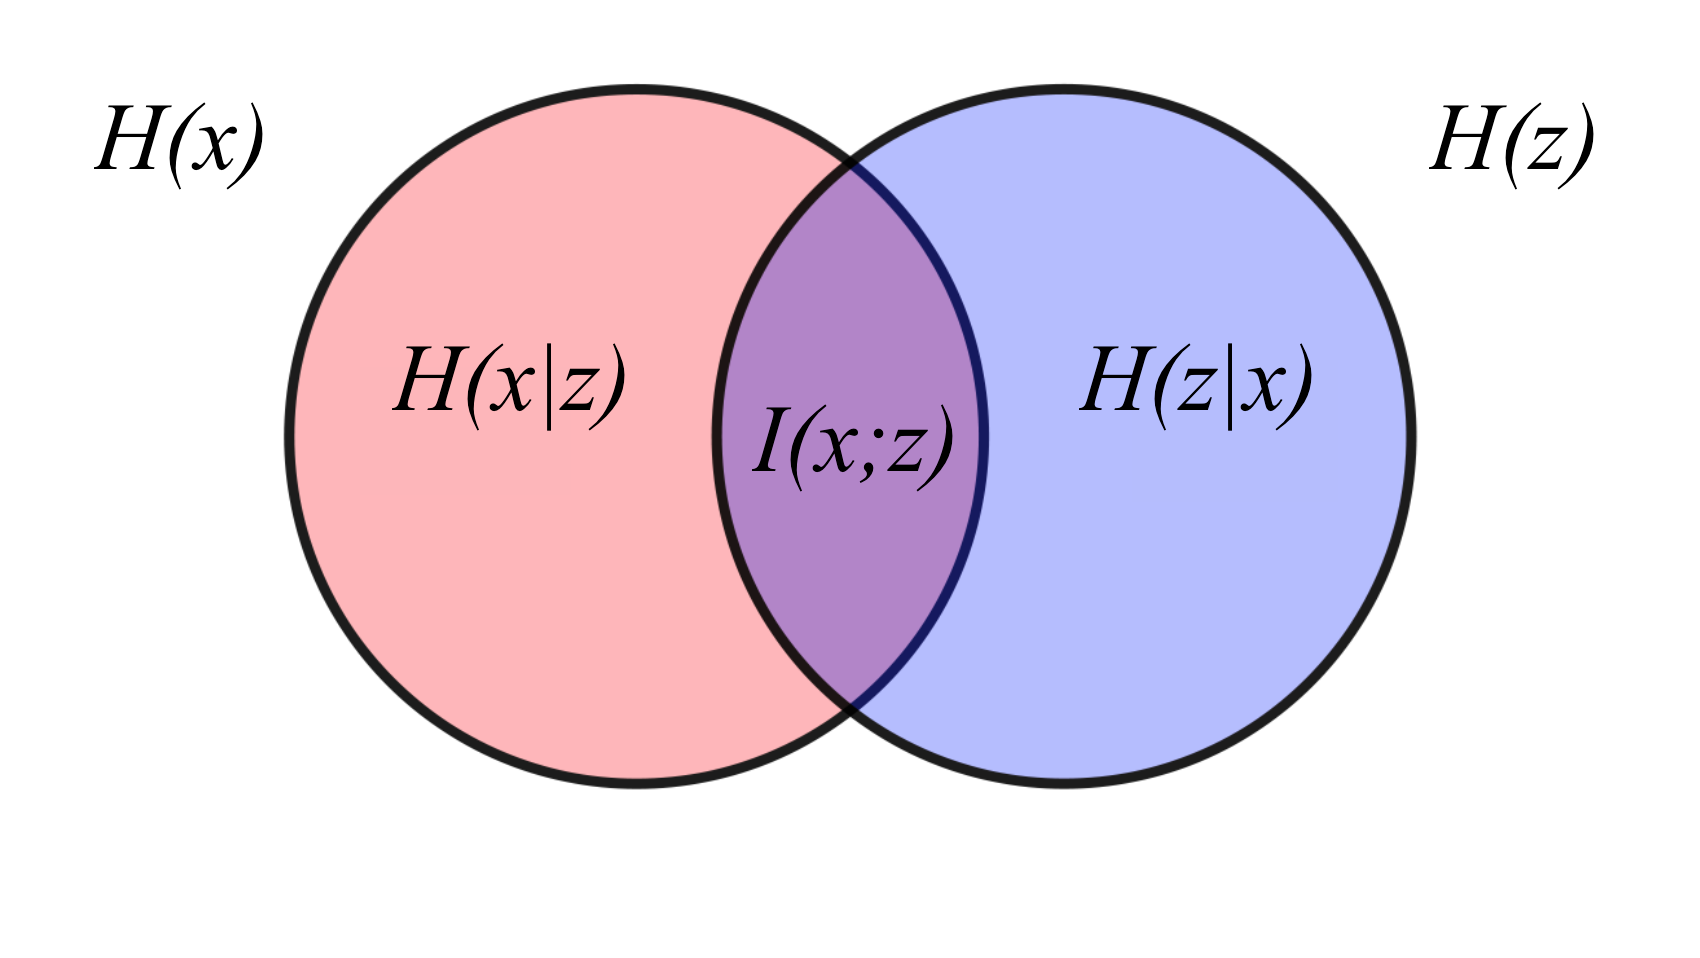
\includegraphics[scale=0.25]{mutual-info}
    \caption{Venn Diagram showing the relationships between the entropies and the conditional entropies of random variables $X$ and $Z$.}
\end{figure}

Since the entropy is a way of measuring ``\emph{how surprising is that an event occurs}'' (this is explained in this document), intuitively the mutual information measures the decrease of uncertainty that we obtain in $X$ when we know that $Z$ has occurred.

Calculating the mutual information between two variables, however, is not an computationally easy problem. Because of this, a way to approach the mutual information maximization is by obtaining lower bounds and maximizing them. Although a few more bounds are proved in this document, we remark the \emph{Contrastive Lower Bound} on the mutual information, which is expressed as follows:
\[
I(X,Z)  \geq - \ell(\theta) + \log N,
\]
where $\ell(\theta)$ refers to the contrastive loss. In short, the \emph{contrastive learning} problem consists of, given elements obtained from one distribution $P$ (considered as positive samples) and elements obtained from a different distribution $Q$ (considered as negative samples), learning how to discriminate between the elements of the different distributions. In order to do this, the recently mentioned contrastive loss is used, which usually takes the form
\[
\ell_{i,j} = -  \log \frac{f(x_i,x_j)}{\sum_{x_k \in X}f(x_i,x_k)},
\] 
where $(x_i,x_j)$ is a positive pair. Intuitively, contrastive loss takes the output of the network for a positive example and calculates its distance (using the function $f$) to an example of the same class and contrasts that with the distance to negative examples. In other words, the loss is low if positive examples are encoded to similar representations and negative examples are encoded to different representations. The use of this contrastive loss maximizing the mutual information had a huge impact on the state of art results of representation learning in 2018 \citep{oord_representation_2019}, achieving very promising results.

However, during the development of this work (around July 2020), this drastically changed. New papers  \citep{chen_simple_2020, grill2020bootstrap} appeared stating that the success of the methods that were maximizing mutual information between the input and its representation was not caused by mutual information, but by the specific form that the contrastive loss has.

With this papers, new frameworks for representation learning appeared. These frameworks provided an ingenious way to apply  the contrastive learning set up to representation learning. This technique consists of presenting different perspectives of the same image to two different encoders (the neural networks that learns how to transform the input to a representation) different \emph{perspectives} (or, being technical, \emph{data augmentations}) of the same image and, later, trying to minimize some sort of distance between these views.  

To achieve this, these perspectives are obtained by applying transformations to the original image. It is shown that the chosen transformations and how to sequence them before passing the transformed image to the neural network really affects the performance of the models.

All this considered, the interest of this work  speaks on its own. Being able to train networks that learn representations that are good enough on its own to perform downstream tasks without needing the supervision of having the labels of the data opens a world of possibilities in many areas. For instance, many insurance companies need to pay their workers to label large amounts of  different insurance bills that they offer to their clients. With the advances presented in this work, these companies would only have to label a very small amount of images to be able to classify the representations obtained by the frameworks.


\section*{Main goals and results achieved}

The main goals of this bachelor's thesis were:
\begin{enumerate}
\item To study, understand and present the basic concepts and properties of \emph{mutual information}, which is in the field of \emph{Information Theory.} Also, related to this, to present some lower bounds that can be used to maximize the mutual information between two random variables.
\item To study the \emph{noise contrastive estimation} problem, and how it is applied to machine learning.

\item To test the most important frameworks that achieve the current state of art results in representation learning. 
\end{enumerate}

The first two goals were successful. For the latter goal, two different frameworks were tested: \lstinline{SimCLR} and \lstinline{BYOL}. 

Different executions were made for each one, trying to find the set of parameters for being able to obtain a high classification accuracy on a specific dataset. The selection of the chosen hyperparameters was argued and the limitations and problems we face are also presented. This way, I gained not only a deep understanding of the representation learning problem and how it is solved, but also in computational capability of the used hardware, so that a plausible future plan could be to improve the results obtained by making use of even better computational resources.

\clearpage
\chapter{Fundamentals}


Underneath each experiment involving any grade of uncertainty there is a \emph{random variable}. This is no more than a \emph{measurable} function between two \emph{measurable spaces}.
A probability space is composed by three elements: $(\Omega, \Alg, \Prob)$. We will define those concepts one by one.

\section{Basic notions}

\begin{ndef}Let $\Omega$ be a non empty sample space. $\Alg$ is a $\sigma-$algebra over $\Omega$ if it is a family of subsets of $\Omega$ that verify that the emptyset is in $\Alg$, and it is closed under complementation and countable unions. That is:
\begin{itemize}
  \item $\emptyset \in \Alg$
  \item If $A \in \Alg$, then $\Omega \backslash A \in \Alg$
  \item If $\{A_i\}_{i \in \mathbb N} \in A$ is a numerable family of $\Alg$ subsets, then $\cup_{i \in \mathbb N} A_i \in \Alg$
\end{itemize}
\end{ndef}


The pair $(\Omega,\Alg)$ is called a \emph{measurable space} To get to our probability space, we need to define a \emph{measure} on the \emph{measurable space}.

\begin{ndef}
Given $(\Omega,\Alg)$, a measurable space, a \emph{measure} $\Prob$ is a countable additive, non-negative set function on this space. That is: $\Prob: \Alg \to \mathbb R_0^+$ satisfying:
\begin{itemize}
  \item $\Prob(A) \geq \Prob(\emptyset) = 0$ for all $A \in \Alg$
  \item $P(\cup_n A_n) = \sum_n P(A_n)$ for any countable collection of disjoint sets $A_n \in \Alg$.
\end{itemize}
\end{ndef}

If $\Prob(\Omega) = 1$, $\Prob$ is a \emph{probability measure} or simply a \emph{probability}. With the concepts that have just been explained, we get to the following definition:

\begin{ndef}
A \emph{measure space} is the tuple $(\Omega, \Alg,\Prob)$ where $\Prob$ is a \emph{measure} on $(\Omega, \Alg)$. If $\Prob$ is a \emph{probability measure} $(\Omega,\Alg,\Prob)$ will be called a \emph{probability space}.
\end{ndef}

Throughout this work, we will be always in the case where $\Prob$ is a probability measure, so we will always be talking about probability spaces. Some notation for these measures must be introduced. Let $A$ and $B$ be two events.
The notation $P(A,B)$ reffers to the probability of the intersection of the events $A$ and $B$, that is: $P(A,B) := P(A\cap B)$.
 It is clear that since $A \cap B = B \cap A$, then $P(A,B) = P(B,A)$. We remark the next definition since it will be important.

\begin{ndef}
Let $A,B$ be two events in $\Omega$. The \emph{conditional probability} of $B$ given $A$ is defined as:
$$
P(B|A) = \frac{P(A,B)}{P(A)}
$$
\end{ndef}



% Introduce here Bayes Theorem
% ------------------------------------------------------------------------------

There is an alternative way to state the definition that we have just made.

\begin{nth}[Bayes' theorem]
Let $A,B$ be two events in $\Omega$, given that $P(B) \neq 0$. Then
$$
P(B|A) = \frac{P(A|B) P(A)}{P(B)}
$$
\end{nth}
\begin{proof}
Straight from the definition of the conditional probability we obtain that:
$$
P(A,B) = P(A|B)P(B)
$$
We also see from the definition that
$$
P(B,A) = P(B|A)P(A)
$$
Hence, since $P(A,B) = P(B,A)$,
$$
P(A|B)P(B) = P(B|A)P(A) \implies P(A|B) = \frac{P(B|A)P(A)}{P(B)}
$$
\end{proof}


However, events might not give any information about another event occurring. When this happens, we call those events to be \emph{independent}. Mathematically, if $A$,$B$ are independent events:
$$
P(A,B) = P(A)P(B)
$$
and as a consequence of this, the conditional probabilty of those events is $P(A|B) = P(A)$. For a finite set of events $\{A_i\}_{i=1}^n$, we say that they are mutually independent if and only if every event is independet of any intersection of the other events. 
That is, if $\{B_i\} \subset \{A_i\}$, then
$$
P\left(\cap_{i = 1}^k B_i \right) = \prod_{i = 1}^k P(B_i) \quad \quad \forall k \leq n
$$

\emph{Random variables} (R.V.) can now be introduced. Their first property is that they are measurable functions. These kind of functions are defined as it follows:

\begin{ndef}
Let $(\Omega_1, \Alg),(\Omega_2, \mathcal B)$ be measurable spaces. A function $f: \Omega_1 \to \Omega_2$ is said to be \emph{measurable} if, $f^{-1}(B) \in \Alg$ for every $B \in \mathcal B$.
\end{ndef}

As a quick note, we can affirm that if $f,g$ are real-valued measurable functions, and $k \in \mathbb R$, it is true that $kf$, $f+g$ , $fg$ and $f/g$ (if $g$ is not the identically zero function) are also \emph{measurable functions}.

We are now ready to define one of the concepts that will lead us to the main objective of this thesis.

\begin{ndef}[Random variable]
Let $(\Omega,\Alg,\Prob)$ be a probability space, and $(E,\mathcal B)$ be a measurable space. 
A \emph{random variable} is a measurable function $X: \Omega \to E$, from the probability space to the measurable space. This means: for every subset $B \in (E,\mathcal B)$, its preimage
$$
X^{-1}(B) = \{\omega : X(\omega) \in B\} \in \Alg .
$$
\end{ndef}

Using that sums, products and quotients of measurable functions are measurable functions, we obtain that \emph{sums, products and quotients of random variables are random variables}.

Let now $X$ be a R.V. The \emph{probability} of $X$ taking a concrete value on a measurable set contained in $E$, say, $S \in E$, is written as:
$$
P_X(S) = P(X \in S) = P(\{a \in \Omega : X(a) \in S\})
$$

A very simple example of random variable is the following:

\begin{nexample}
  Consider tossing a coin. The possible outcomes of this experiment are \emph{Heads or Tails}. Those are our random events. We can give our random events a possible value. For instance, let \emph{Heads} be $1$ and \emph{Tails} be $0$. Then, our random variable looks like this:
  \begin{equation*}
      X  = \left\{ \begin{aligned}
  1 & \text{ if we obtain heads} \\
  0 & \text{ if we obtain tails}
\end{aligned}\right.
  \end{equation*}

\end{nexample}

In the last example, our random variable is \emph{discrete}, since the set $\{X(\omega): \omega \in \Omega\}$ is finite.
 A \emph{Random Variable} can also be \emph{continuous}, if it can take any value within an interval.\\


\section{Expectation of a random variable}

\begin{ndef}
The \emph{cumulative distribution function } $F_X$ of a real-valued random variable $X$ is its probability of taking value below or equal to $x$. That is:
$$
F_X(x) = P(X \leq x) = P(\{\omega : X(\omega) \leq x\}) = P_X((-\infty,x]) \quad \forall x \in \mathbb R
$$
\end{ndef}

Depending on the image of a random variable $X$, we can difference between certain types of random variables. If the image $\mathcal X$ of $X$ is countable, we call it a \emph{discrete} random variable. Its \emph{probability mass function} gives the
probability of the r.v. being equal to a certain value:
$$
p(x) = P(X = x).
$$
If the image $\mathcal X$ of $X$ is uncountable and real, then $X$ is a \emph{continuous} random variable. In this case there might exist a non-negative Lebesgue-integrable function $f$ such that:
$$
F_X(x) = \int_{\infty}^x f(t) dt,
$$
called the \emph{probability density function} of $X$.\\

We are now ready to introduce the \emph{expectation} of a random variable.

\begin{ndef}[Expectation of a \emph{R.V.}]
Let $X$ be a non negative random variable on a probability space $(\Omega,\Alg,\Prob)$. The expectation $E[X]$ of $X$ is defined as:
$$
E[X] = \int_\Omega X(\omega) \ dP(\omega)
$$
\end{ndef}
The expectation of a random variable will be also denoted as $\mu$. Now, if $X$ is generic \emph{R.V}, the expectation is defined as:
$$
E[X] = E[X^+] - E[X^-]
$$
where $X^+,X^-$ are defined as it follows:
$$
X^+(\omega) = \max(X(\omega),0) \quad \quad  \quad \quad X^-(\omega) = \min(X(\omega),0)
$$

The \emph{expectation} $E[X]$ of a \emph{random variable} is a linear operation. That is, if $\mathcal Y$ is another random variable, and $\alpha,\beta \in \R$, then
$$
E[\alpha X + \beta \mathcal Y] = \alpha E[X] + \beta E[\mathcal Y]
$$
this is a trivial consequence of the linearity of the \emph{Lebesgue integral}.

As a note, if $X$ is a \emph{discrete} random variable and $\X$ is its image, its expectation can be computed as:
$$
E[X] = \sum_{x \in \X} x  P_X(x)
$$
where $x$ is each possible outcome of the experiment, and $P_X(x)$ the probability under the distribution of $X$ of the outcome $x$. The expression given in the definition before generalizes this particular case.

Using the definition of the \emph{expectation} of a random variable, we can approach to the \emph{moments} of a random variable.

\begin{ndef}
If $k \in \N$, then $E[X^k]$ is called the $k-th$ moment of $X$.
\end{ndef}
If we take $k = 1$, we have the definition of the \emph{expectation}. It is sometimes written as $m_X = E[X]$, and called the \emph{mean}. We use the \emph{mean} in the definition of the variance:

\begin{ndef}
Let $X$ be a random variable. If $E[X^2] < \infty$, then the \emph{variance} of $X$ is defined to be
$$
\Var(X) = E[(X - m_X)^2] = E[X^2] - m_X^2 
$$
\end{ndef}

Thanks to the linearity of the \emph{expectation} of a random variable, it is easy to see that, if $a,b \in \R$, then
$$
Var(aX + b) = E[(aX + b) - E[aX + b])^2] = a^2E[(X - m_X)^2] = a^2 \Var(X)
$$



Usually, when it comes to applying these concepts to a real problem, we will be looking at multiple variables. We would like to have a collection of random variables each one representing one of this variables.
In order to set the notation for these kinds of situations, we will introduce \emph{random vectors}.

\begin{ndef}
  A random vector is a row vector $\rvc$ whose components are real-valued random variables on the same probability space $(\Omega,\Alg,P)$.
\end{ndef}

The probability distribution of a random variable can be extended in to the \emph{joint probability distribution} of a random vector.

\begin{ndef}
Let $\rvc$ be a random vector. The \emph{cumulative distribution funcion} $F_{\rv} : \R^n \to [0,1]$ of $\rv$ is defined as:
$$
F_{\rv}(x) = P(X_1 \leq x_1 , \dots, X_n \leq x_n).
$$
\end{ndef}

We also name it \emph{multivariate distribution}.  We explained before the independence of a pair of events. Using the cumulative distribution function, we can now define the independence between random variables.
\begin{ndef}
A finite set of $n$ random variables $\{X_1,\dots,X_n\}$ is mutually independent if and only if, for any sequence $\{x_1,\dots,x_n\}$, the events $\{X_1 \leq x_1\}, \dots, \{X_n \leq x_n\}$ are mutually independent. 
Equivalently, this finite set is mutually independent if and only if:
$$
F_{X_1,\dots, X_n}(x_1,\dots,x_n) = F_{X_1}(x_1) \dots F_{X_n}(x_n) \quad \quad \text{ for all } x_1,\dots,x_n.
$$
\end{ndef}


We can also extend the notion of expectation to a random vector. Let $\rvc$ be a random vector and assume that $E[X_i]$ exists for all $i \in \{1, \dots, n \}$. The expectation of $\rv$ is defined as the vector containing the expectations of each individual random vector, that is:
$$
E[\rv] = \left[ \begin{array}{c} 
E[X_1]\\
\vdots\\
E[X_n]
\end{array} \right]
$$

To generalize the variance of a random variable, we have to build the following matrix.

\begin{ndef}
Let $\rvc$ ve a random vector. Then, the \emph{covariance matrix} of $\rv$ is defined as:
$$
\Sigma = \mathrm{Cov}(\rv) = E[(\rv - \mu_\rv)(\rv - \mu_\rv)^T] = \left ( \begin{array}{ccc} 
  \sigma_{11} & \cdots & \sigma_{1n}\\
  \vdots & \ddots & \vdots \\
  \sigma_{n1} & \cdots & \sigma_{nn}
  \end{array} \right )
$$
where $\sigma_{ij} = Cov(X_i,X_j) = E[(X_i - \mu_i)(X_j - \mu_j)] = \sigma_{ji}$.
\end{ndef}


It can also happen that, given a \emph{random vector}, we would like to know the probability distribution of a few of its components. That is called the \emph{marginal distribution}.

\begin{ndef}[Marginal Distribution]
Let $\rvc$ be a random vector. The marginal distribution of a subset of $\rv$ is the probability distribution of the variables contained in the subset. 
\end{ndef}
In the simple case of having two random variables, e.g. $X_1$ and $X_2$, then the marginal distribution of $X_1$ is:
$$
P(x) = \int_{X_2} P(x_1,x_2) dx_2.
$$


\label{Chapter:distributions}

We have introduced the concepts of \emph{random variable},  \emph{random vector} and its \emph{probability distribution}. We will explain some concepts related to the latter ones.

\begin{ndefC}
    The \emph{mode} of a distribution is the value at which the probability mass function takes its maximum value. That is, the value that is most likely to be sampled.
\end{ndefC}

Distributions can be \emph{unimodal}, when their distribution has a single peak, \emph{bimodal} when their distribution has two peaks, and \emph{multimodal} when the number of peaks is equal or greater to $2$. 

\begin{nexample}
We can simulate the two following distributions:
\begin{enumerate}
    \item The distribution of the marks obtained in a test by the students of certain class.
    \item The distribution of the height of the plants from three different species.
\end{enumerate}
The result is the following:
\begin{figure}[H]%!htb]
    \minipage{0.45\textwidth}
      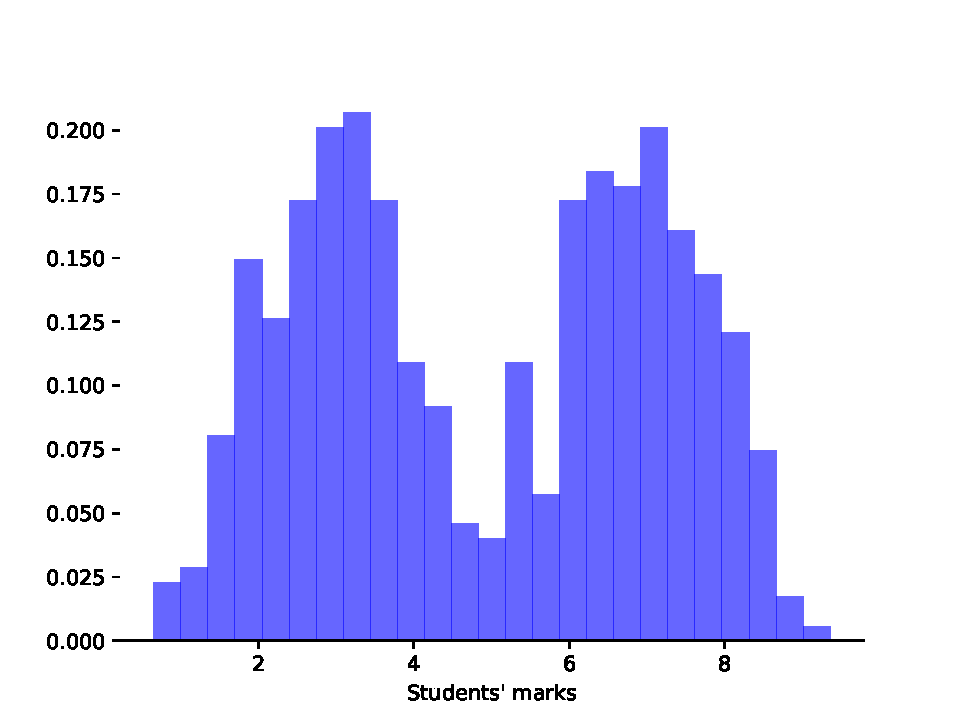
\includegraphics[width=\linewidth]{media/bimodal.pdf}
      \caption{Bimodal Distribution}\label{fig:linCM}
    \endminipage\hfill
    \minipage{0.45\textwidth}%
      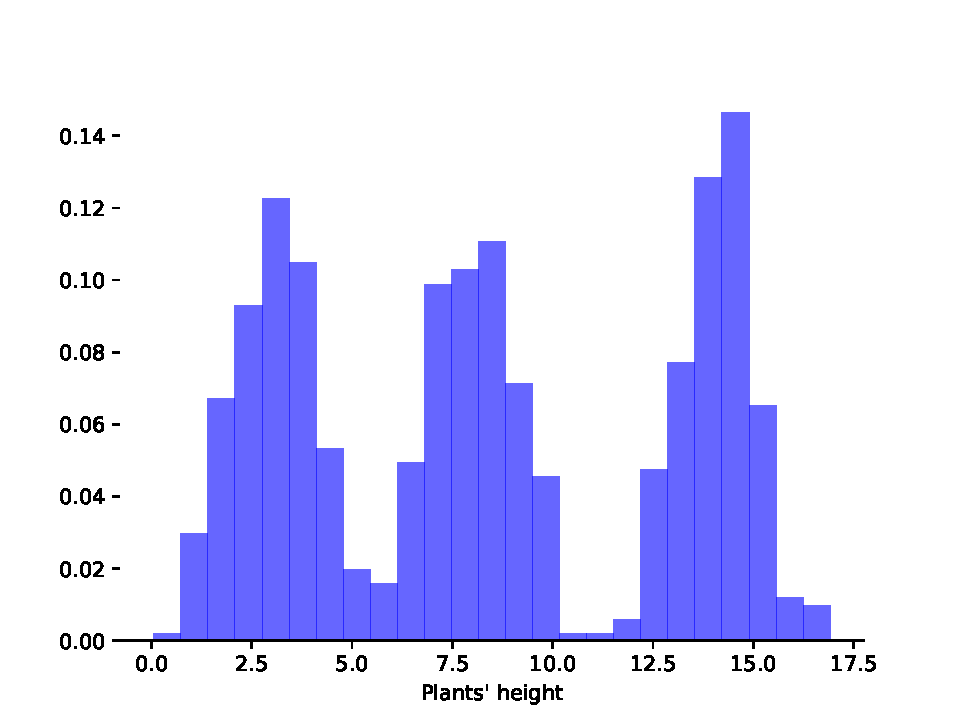
\includegraphics[width=\linewidth]{media/multimodal.pdf}
      \caption{Plants' height}\label{fig:RFCM}
    \endminipage
    \caption{Examples of bimodal and multimodal distributions.}
    \end{figure}
\end{nexample}


Now, given two distributions, we would like to determine how different they are from each other.
In order to compare them, we enunciate the definition of the Kullback-Leibler divergence.

\begin{ndefC}
Let $P$ and $Q$ be probability distributions over the same probability space $\Omega$. Then, the Kullback-Leibler divergence is defined as:
$$
D_{KL}(P \ || \ Q) = E_P\left[\log{\frac{P(x)}{Q(x)}}\right].
$$
\end{ndefC}
It is defined if, and only if, $P$ is \emph{absolutely continuous with respect to} $Q$, that is, if $P(A) = 0$ for any $A$ subset of $\Omega$ where $Q(A) = 0$.
 There are some properties of this definition that must be stated. 

\begin{nprop}
If $P,$ $Q$ are two probability distributions over the same probability space, then $D_{KL}(P|Q) \geq 0$.
\end{nprop}
\begin{proof}
Firstly, note that if $a \in \R^+$, then $\log \ a \leq a-1$. Then:
\begin{align*}
-D_{KL}(P \ || \ Q) & = - E_P\left[\log{\frac{P(x)}{Q(x)}}\right] \\
             & = E_P\left[\log{\frac{Q(x)}{P(x)}}\right] \\
             & \leq E_P\left[\left(\frac{Q(x)}{P(x)} - 1\right)\right]\\
             & = \int P(x) \frac{Q(x)}{P(x)} \mathop{dx} -1 \\
             & = 0.
\end{align*}
So we have obtained that $-D_{KL}(P\ ||\ Q) \leq 0$, which implies that $D_{KL}(P\ || \ Q) \geq 0$.
\end{proof}
As a corollary of this proposition, we can affirm that $D_{KL}(P\ ||\ Q)$ equals zero if and only if $P = Q$ almost everywhere. 
We will also remark the discrete case, as it will be used later. Let $P,Q$ be discrete probability distributions defined on the same probability space $\Omega$. Then, 
$$
D_{KL}(P\ ||\ Q) = \sum_{x \in \Omega} P(x) \log \left( \frac{P(x)}{Q(x)}\right).
$$

\section{Examples of distributions}

Let us present some examples o common distributions. They will be used further in this document.

\subsection{Bernoulli}

Think for a moment that you want to model the possible outcomes of an experiment with two possibilites: sucess or failure. Imagine also that you already know that in your experiment there is a probability $p$ of 
achieving success. That is the intuitive idea of a Bernoulli distribution. We can define it more formally as follows: 

The \emph{Bernoulli distribution} is a discrete probability distribution of a random variable that takes two values, $\{0,1\}$, with probabilities $p$ and $q = 1-p$, respectively. We will say that our distribution is a $Bern(p)$.

If $k$ is a possible outcome, we can define
the probability mass function $f$ of a Bernoulli distribution as:
$$
f(k,p) = 
\begin{cases} 
p, \quad & \text{ if } k=1,\\
1-p, \quad & \text{ if } k = 0.
\end{cases}
$$
Using the expression of the mean for discrete random variables, we obtain that $E[X] = p$ and 
$$
\Var[X] = E[X^2] - E[X]^2 = E[X] - E[X]^2 = p-p^2 = p(1-p) = pq.
$$

As a note, this is just a particular case of the \emph{Binomial distribution} with $n=1$.

\subsection{Gaussian Distribution}

The Gaussian (or normal) distribution is used to represent real-valued random variables whose distributions are not known.
Its importance relies in the fact that, using the \emph{central limit theorem}, we can assume that the average of many samples of
a random variable with finite mean and variance is a random variable whose distribution converges to a normal distribution as the number of samples increases.

\begin{ndef}
We say that the real valued random variable $X$ follows a \emph{normal distribution} of parameters $\mu,\sigma\in \R$ if, and only if,
its probability density function exists and it is determined by
\begin{equation}\label{gaussian:function}
f(x) = \frac{1}{\sigma \sqrt{2\pi}}e^{-\frac{1}{2}\left( \frac{x - \mu}{\sigma}\right)^2},
\end{equation}
where $\mu$ is the mean and $\sigma$ is its standard deviation. We denote this normal distribution as $X \sim \mathcal N (\mu,\sigma)$.
\end{ndef}

The particular case where $\mu = 0$ and $\sigma = 1$ is widely used in statistics. In this case, the density function is simpler:
\[
f(x) = \frac{1}{\sqrt{2\pi}}e^{-\frac{1}{2}x^2}.
\]

A remarkable property of these distributions is that, if $f : \R \to \R$ is a real-valued function defined 
as $f(x) = ax+b$, then $f(X) \sim \mathcal N (a\mu + b, \abs{a} \sigma)$.\\

In the same way that we extended random variables to random vectors, we can extend the normal distribution to a multivariate
random distribution.

\begin{ndef}
We say that a random vector $\bm{X} = (X_1,\dots,X_n)$ follows a multivariate normal distributions of parameters
$\mu \in \R^n$, $\Sigma \in \mathcal M_N(\R)$ if, and only if, its probabity density function is:
\begin{equation*}\label{gaussian:function:vector}
f(x) = \frac{1}{\sqrt{\det(2\pi \Sigma)}}e^{-\frac{1}{2}(x - \mu )^T \Sigma^{-1} (x-\mu)}.
\end{equation*}
It is denoted $X \sim \mathcal N(\mu, \Sigma)$.
In this case, $\mu$ is the mean vector of the distribution and $\Sigma$ denotes the covariance matrix.  
\end{ndef}

\clearpage
\section{Statistical Inference}
Statistical inference is the process of deducing properties of an underlying distribution by analyzing the data that it is available. With this purpose, techniques like deriving estimates and testing hypotheses are used. 

Inferential statistics are usually contrasted with descriptive statistics, which are only concerned with properties of the observed data. The difference between these two is that in inferential statistics, we assume that the data comes from a larger
population that we would like to know.

In \emph{machine learning}, subject that concerns us the most, the termi inference is sometimes used to mean \emph{make a prediction by evaluating an already trained model}, and in this context, inferring properties of the model is refered as \emph{training or learning}.

\section{Parametric Modeling}

In the following chapters, we will be trying to estimate density functions in a dataset. To do this we will be using \emph{parametric models}. We say that a \emph{parametric model}, $p_\theta(x)$, 
is a family of density functions that can be described using a finite numbers of parameters $\theta$. We can get to the concept of \emph{log-likelihood} now.

\begin{ndef}
The \emph{likelihood} $\mathcal L(\theta | x)$ of a parameter set $\theta$ is a function that measures how plausible is $\theta$, given an observed point $x$ in the dataset $\D$. It is defined as the value of the 
density function parametrized by $\theta$ at $x$. That is:
$$
\mathcal L(\theta|x) = p_\theta(x).
$$
\end{ndef}

In a finite dataset $\D$ consisting of independent observations, we can write:
\[
\mathcal L(\theta | X) = \prod_{x \in D} p_\theta(x).
\]

This can be computationally hard to work with, so the log-likelihood is often used instead.

\begin{ndef}
Let $\D$ be a dataset of independent observations and $\theta$ a set of parameters. Then, we define the \emph{log-likelihood} $\ell$ as the sum of the logarithms of the evaluations of $p_\theta$ in each $x$ in the dataset. That is:
\[
\ell (\theta | X) = \sum_{x \in \D} \log p_\theta(x).
\]
\end{ndef}

Our goal would be to find the optimal value $\hat{\theta}$ that maximizes the likelihood of observing the dataset $\D$. We get to the following definition:

\begin{ndef}
    We say that $\hat{\theta} = \hat\theta (\D)$ is a \emph{maximum likelihood estimator}(MLE) for $\theta$ if  
    $$
    \hat\theta \in \argmax_{\theta} \mathcal L(\theta | \D)
    $$
    for every observation $\D$. 
\end{ndef}

\section{Minimal sufficient statistics}

In parametric modeling, the goal was to determine the density function under a distribution. Another interesting task can be determining specific parameters or quantitys related to a distribution, given a sample $X = (x_1,\cdots,x_n)$.

\begin{ndef}
    A \emph{statistic} is a measurable function of the data. That is, if $T : \Omega \to \mathbb T$ is measurable, then $T(X)$ is a statistic.
\end{ndef}

However, not all statistics will provide useful information for the statistical inference problem. We would like to find statistics that provide relevant information.

\begin{ndef}
    Let $X \sim P_\theta$. Then, the statistic $T(X) = T : (\Omega, \Alg) \to (\mathbb T, \mathcal B)$, is sufficient for a family of parameters $\{P_\theta \ : \ \theta \in \Theta \}$ if the conditional distribution of $X$, given $T = t$, is indepentent of $\theta$.\\

    Alternatively, we can say $T(X)$ is sufficient for $\theta$ if its mutual information with $\theta$ equals the mutual information between $X$ and $\theta$, that is:
    $$
    I(\theta, X) = I (\theta, T(X))
    $$
\end{ndef}

The easiest example of a sufficient statistic is the mean $\mu$ of a gaussian distribution with known variance. Oppositely, the \emph{median} of an arbitrary distribution
is not sufficient for the mean since, even if the median of the sample is known, more information about the mean of the population can be obtained from the mean of the sample itself.

Although it will not be shown in this document, sufficient statistics are not unique. In fact, if $T$ is sufficient, $\psi(T)$ is sufficient for any bijective mapping $\psi$. It would be interesting to find a sufficient statistic $T$ that is \emph{the smallest} of them.

\begin{ndef}
    A sufficient statistic $T$ is minimal if, for every sufficient statistic $U$, there exists a mapping $f$ such that $T(x) = f(U(x))$ for any $x \in \Omega$.
\end{ndef}
\section{Introduction to Deep Learning}
\label{Chapter:Introduction:DL}

In order to be able to understand the chapters that will come later in this document, it is important to make a brief introduction of what \emph{Deep Learning}(DL) refers to. Deep learning is included in the field of Machine Learning, which is also included in the field of general Artificial Intelligence.

In Chapter \ref{Chapter:Intro:Rep:Learning}, an intuitive definition of what Machine Learning is was given. We said that ML studies the algorithms that improve from experience. Tom M. Mitchell \citep{mitchell_machine_1997} provided a more formal definition of what \emph{learning from experience} means:

\begin{ndefC}
A computer program is said to \emph{learn} from experience $E$ with respect some class of tasks $T$ and performance measure $P$, if its performance at tasks in $T$, as measured by $P$, improves with experience $E$.
\end{ndefC}

We would also like to have a DL definition. In \cite{deng_deep_2014}, multiple similar definitions are given. We present here the simplest of them:

\begin{ndefC}
\emph{Deep Learning} is a class of ML learning techniques that exploit many layers of non-linear information processing for supervised or unsupervised feature extraction and transformation, and for pattern analysis and classification.
\end{ndefC}

Usually, these techniques are based on the biologically inspired \emph{neural networks}(NNs), which consists in several connected units: the \emph{neurons}. Each neuron is basically a Perceptron, which is a is a weighted sum followed by a non-linear function, called an \emph{activator} in the ML context. Formally, the output of each neuron is 
\[
y = \phi\left(w_0 +\sum_{i = 1}^N w_i x_i \right) .   
\]
There are many activation functions, but the following examples must be remarked:
\begin{itemize}
\item Sigmoid. The sigmoid function is defined as follows:
\[
\phi(x) = \frac{1}{1+ e^{-x}}.
\]
This is one of the most common used activation functions. It is differentiable, monotonic and smooth. One of its main disadvantages is that at the right part of the function, the change in the values that the function takes converges to zero, so we get to the \emph{vanishing gradient} problem and the learning is minimal.

\begin{figure}[H]
    \centering
    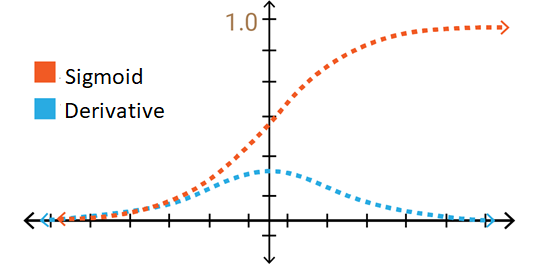
\includegraphics[width=0.5\linewidth]{sigmoid}
    \caption{Sigmoid. Image from \href{https://xzz201920.medium.com/activation-functions-linear-non-linear-in-deep-learning-relu-sigmoid-softmax-swish-leaky-relu-a6333be712ea}{this Medium article}. } \label{fig:sigmoid}
\end{figure}

\item Hyperbolic Tangent. This function is defined as follows:
\[
\phi(x) = \operatorname{tanh}(x) =  \frac{e^x - e^{-x}}{e^x + e^{-x}}.    
\]
This activation function has a small advantage over the sigmoid: its derivative is more steep, which means it can get more value and the learning can be more efficient.

\begin{figure}[H]
    \centering
    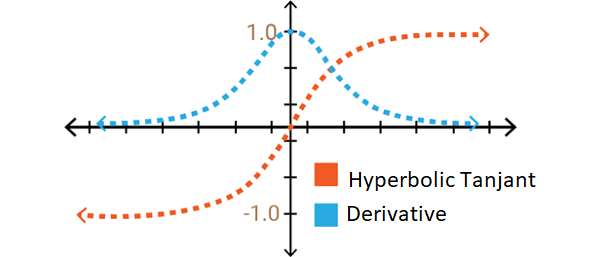
\includegraphics[width=0.6\linewidth]{tanh}
    \caption{Hyperbolic Tangent. Image from \href{https://xzz201920.medium.com/activation-functions-linear-non-linear-in-deep-learning-relu-sigmoid-softmax-swish-leaky-relu-a6333be712ea}{this Medium article}. } \label{fig:tanh}
\end{figure}

\item Rectified Linear Unit (ReLU). This function takes the following form:
\[
\phi(x) = \max\left(0,x\right).    
\]
ReLu is highly computationally efficient and non-linear. Its main problem is that when the inputs approach zero or are negative, the network can not perform back propagation and can not learn.

\begin{figure}[H]
    \centering
    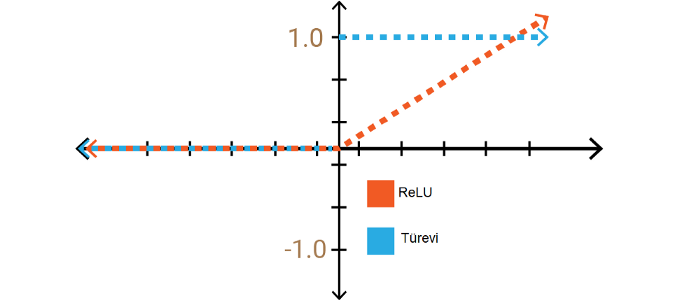
\includegraphics[width=0.6\linewidth]{relu}
    \caption{ReLU. Image from \href{https://xzz201920.medium.com/activation-functions-linear-non-linear-in-deep-learning-relu-sigmoid-softmax-swish-leaky-relu-a6333be712ea}{this Medium article}. } \label{fig:relu}
\end{figure}
\end{itemize}



\section{Neural Networks}

Using neurons and activation functions, we can formally define NNs. A NN with $L$ hidden layers is a deterministic non-linear function $f$, parametrized by a set of matrices $W = \{W_0,\cdots,W_L\}$ and non-linear activation functions $\{\phi_0,\cdots,\phi_L\}$. Given an input $x$, the output $y$ of the network is calculated as follows:
\[
h_0 = \phi_0\left(W_0^Tx\right), \cdots, h_l = \phi_l\left(W_l^T h_{l-1}\right),\cdots, y = \phi_L\left(W_L^T h_{L-1}\right).
\]
Having a NN, we consider it \emph{deep} when the number of hidden layers (and, consequently, the number of matrices) is considered high. 

Neural networks use loss functions, which define how well the output returned by the network matches the real output, reducing the learning problem to an optimization problem. The problem is finding $W^{\operatorname{opt}}$, such that
\[
W^{\operatorname{opt}}   = \argmin_{w} \sum_{n = 1}^N l(y_n, f_w(x_n)),
\]
where $\mathcal D = \{(x_n,y_n)\}$ is a dataset.

This problem is solved using a variant of \emph{stochastic gradient descent (SGD)}. This algorithm involves the computation of the loss function derivatives respect to the network parameters, and updates the parameters using this derivatives. Specifically, the parameters are updated as follows:
\[
W_{t+1} = W_t + \eta \nabla f(W_t),
\]
where $\eta \in \R^+$ is a small constant called the \emph{learning rate}. This algorithm guarantees convergence to local minimums of $f$ and, if $f$ is convex, the algorithm converges to a global minimum.

The last comment about neural networks is that, since the weights $W = \{W_0,\cdots,W_L\}$ are constantly updated, the derivatives have to be computed repeatedly. The computational cost of this is quite high. \emph{Backpropagation} was born to calculate the derivatives of the weights much faster. The intuitive idea is that the gradient of the layer $l$ is computed using the gradient of the layer $l+1$ using the chain rule.

Understanding both SGD and Backpropagation is crucial for understanding how NNs  work. However, in the experimentation part of this work we will focus on researching how a few hyperparameters affect the results of the proposed frameworks, so no further explanation on these important concepts will be provided.

\section{Convolutional Neural Networks}

Convolutional Neural Networks (CNNs) are a specific type of Neural Networks. The difference that we have between CNNs and NNs is that CNNs assume that the inputs have local dependencies. For instance, using an image, a CNN assumes (most of the time correctly) that given a pixel $x_{ij}$ of an input $x$, the neighbours of this pixels will have similar values or intensities. This allows us to encode certain properties into the architecture of the network.

If we use colored images, the input of the CNNs are 3-dimensional volumes, which will be transformed in some layers to other 3-dimensional volumes. In order to do this we have different types of layers, remarking \emph{convolutional} layers, \emph{pooling} layers and \emph{fully connected} layers. The most important ones are convolutional layers.

Convolutional layers receive a \emph{tensor} with shape $k \times n \times m \times c$, which means that the layer receives $k \in \mathbb N$ inputs of sizes $n \times m \times c$.  After the convolutional layer, the input has shape $k \times n' \times m' \times c'$, where $n'$ can be different from $n$ (respectively $m',c'$). One convolutional layer can apply one or several filters to the same input, producing different 2-dimensional activation maps that are stacked along the depth dimension to produce the output.

Formally, a convolution is the process of adding each element of the image to its local neighbours, weighted by a kernel. That is in our case performing a dot product between the input and the filter. We obtain
\[
g(x,y) = \omega \star f(x,y) = \sum_{dx = -a}^a \sum_{dy = -b}^b \omega(dx,dy)f(x+dx,y+dy),    
\]
where $g(x,y)$ is the pixel $(x,y)$ of the filtered image, $f(x,y)$ is the same pixel in the original image, and $\omega$ is the filter kernel. Depending on the filter kernel, the result will be different. 
\begin{nexample}
If we want to produce noise reduction in an image, we use Gaussian Blur, which kernel is calculated by a Gaussian function like the one in Equation \ref{gaussian:function}. For instance, a $3\times 3 $ gaussian kernel would approximately be:
\[
\frac{1}{16}\begin{bmatrix}
    1 & 2 & 1\\
    2 & 4 & 2\\
    1 & 2 & 1
\end{bmatrix}.
\]
\end{nexample}

\subsection{ResNet}

To finish with this introduction to CNNs, we will present a widely used CNN architecture. Since CNNs appeared, people tried to build such deep networks that were very hard to train. When deeper networks start converging, a degradation problem ocurred: with the network depth increasing, accuracy gets saturated and then it degraded rapidly. \emph{ResNet} \citep{he2015deep} brought and end to this problem, allowing the training of very deep models with up to hundreds of layers.

In the paper, they mentioned that if $\mathcal H(x)$ is the underlying map of a sequence of layers and knowing that it can be asymptotically approximated, we can also approximate its residuals
\[
\mathcal F(x) = \mathcal H(x) - x.    
\]
Then, the original function becomes $\mathcal F(x) + x$. In order to achieve this, they introduced the \emph{Residual Block}, a block of layers that introduces skip or shortcut connections that makes it easy for networks to represent the identity mapping. We can see one of this blocks depicted in Figure \ref{fig:resnet:block}.

\begin{figure}[H]
    \centering
    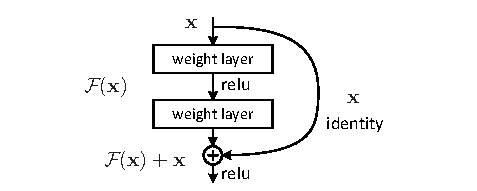
\includegraphics[width=0.6\linewidth]{block}
    \caption{Residual Block. Image from \cite{he2015deep} } \label{fig:resnet:block}
\end{figure}

Usually, ResNet comes accompanied by a number (e.g. \emph{Resnet-50}), that indicates the number of layers it has. Usually, a \emph{batch normalization} is used after each convolution and ReLU is used at the end of each group of layers.

\begin{table}[H]
    \label{arch:resnet:18}
    \centering
    \begin{tabular}{llc}
    Layers                      & Output Size                     & Resnet 18                                                                     \\ \hline
    $conv1$                     & $112\times112$                  & $7 \times 7, \ 64$, stride 2                                                  \\
    \multirow{2}{*}{$conv2\_x$} & \multirow{2}{*}{$56 \times 56$} & $3 \times 3$ max pool, stride 2                                               \\
                                &                                 & $\begin{bmatrix}3 \times 3 , & 64 \\ 3 \times 3,& 64 \end{bmatrix} \times 2$  \\
    $conv3\_x$                  & $28 \times 28$                  & $\begin{bmatrix} 3\times 3, & 128 \\ 3\times 3, & 128 \end{bmatrix} \times 2$ \\
    $conv4\_x$                  & $14 \times 14$                  & $\begin{bmatrix} 3\times 3, & 256\\ 3\times 3, & 256\end{bmatrix} \times 2$   \\
    $conv5\_x$                  & $7 \times 7$                    & $\begin{bmatrix} 3\times 3, & 512\\ 3\times 3, & 512\end{bmatrix} \times 2$   \\
                                & $1\times 1 $                    & average pool, 1000-d fc, softmax                                             
    \end{tabular}
    \caption{Resnet 18 architecture.}
    \end{table}

For instance, having a look at the Table \ref{arch:resnet:18}, in the convolution block \emph{conv\_2}, we have two convolutions 
\clearpage
\chapter{Information theory fundamentals}
\section{Definition}
Intuitively, if $x$ is a datapoint in a dataset $\D \subset \R^d$, a \emph{representation} of $x$ is a vector $r \in \R^n$ (usually, $n \leq d$), that shares information with the datapoint $x$. Representations are very often used in Machine Learning (ML).

Obtaining good representations of data is one of the most important tasks in ML. 
Recently, it has been discovered that maximizing the \emph{mutual information} between two elements in our data can give us good representations for our data.
In this section, \emph{information theory} notions will be presented, in order to use them in our ML models. This will provide a theoretical solid base for
the notions explained later.


The \emph{mutual information} concept is based on the \emph{Shannon entropy}, which we will introduce first, along with some basic properties of it. The Shannon entropy is a way of measuring the uncertainty in a random variable. 
Given an event $\mathcal A \in \Alg$, $P$ a probability measure and $P[\A]$ the probability of $\mathcal A$, we can affirm that 
$$
\log\frac{1}{P[\mathcal A]}
$$
describes \emph{"how surprising is that $\A$ occurs"}. Clearly, then, 
\begin{itemize}
\item If $P[\A]= 1$, then we have $\log 1 = 0$, which would indicate that it is not a surprise that $\A$ occurred.

\item On the other hand, if $P[A]\to 0$, then we have $\log(+\infty)$, which will surely be a big number indicating great surprise that $\A$ occurred.
\end{itemize}

With this motivation, we get to the following definition.
\begin{ndef}
Let $X$ be a discrete random variable with image $\X$. The \emph{Shannon entropy}, or simply \emph{entropy}  $H(X)$ of $X$ is defined as:
$$
H(X) = E_X\left[\log\frac{1}{P_X(X)}\right] =  \sum_{x \in \X} P_X(x) \log\frac{1}{P_X(x)}.
$$
\end{ndef}
The \emph{entropy} can trivially be expressed as:
$$
H(X) = - \sum_{x \in \X}P_X (x)\log P_X(x).
$$

This simple example, \citep{cover_elements_1991}, even though it is very simple, it is very illustrative for our definition:

%http://www.cs.columbia.edu/~vh/courses/LexicalSemantics/Association/Cover&Thomas-Ch2.pdf
\begin{nexample}
    \label{example:entropy}
Let $X \sim Bern(p)$. Then, the entropy of $X$ is:
\[
H(X) = -p \log p - (1-p) \log(1-p)) = H(p),
\]
since $H$ only depends on $p$. In Fig. \ref{example:entropy} we can see a representation of this function. We appreciate that in this case, $H$ is concave and equals $0$ if $p \in \{0,1\}$, which are the values of $p$ that give us no uncertainty. The maximum uncertainty is obtained when $p=\frac{1}{2}$, where we do not know what to expect as an outcome from our random variable $X$.

\begin{figure}[H]
    \label{fig:example:entropy}
    \centering
    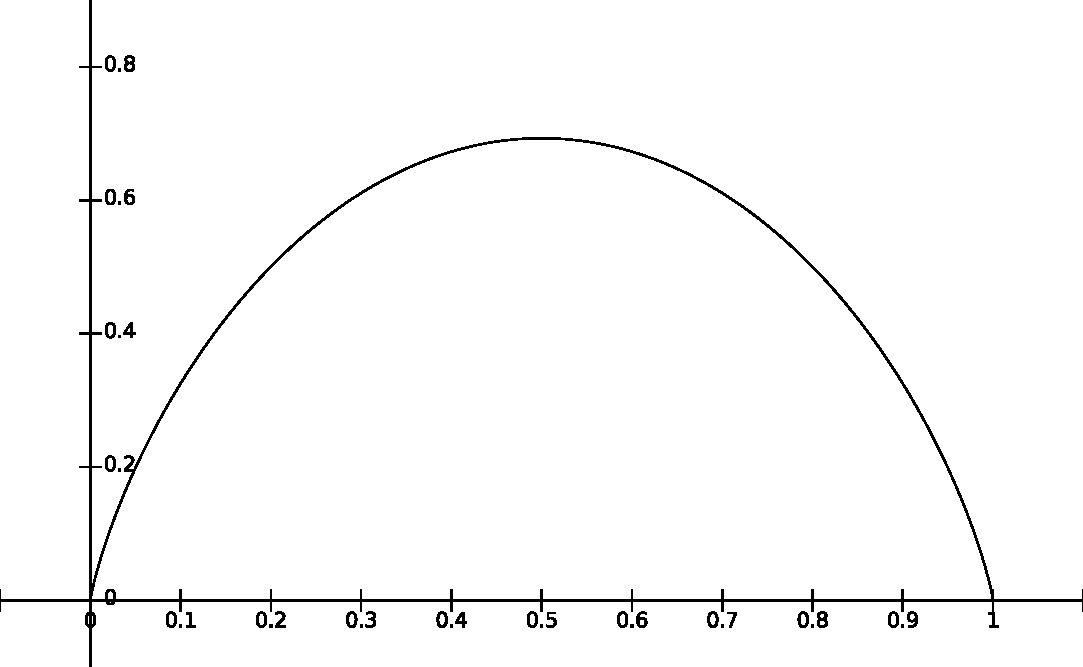
\includegraphics[scale=0.4]{Entropy.pdf}

      \caption{Representation of $H(p)$ in the example \ref{example:entropy}.}
\end{figure}

\end{nexample}
It can also be proven that, in general, the entropy is concave. 


\section{Properties of the entropy. Conditional entropy}

There are some properties of the \emph{entropy} that must be remarked, since they will extend to properties of the mutual information.


\begin{nprop}\label{entr:prop:1}
    Let $X$ be a random variable with image $\X$. If $|\X|$ is the cardinal of $\X$, then
    $$
0 \leq H(X) \leq \log(|\X|).
    $$
\end{nprop}
\begin{proof}
    Since $\log y$ is concave on $\R^+$, by Jensen's inequality ( see Appendix \ref{APPENDIX:A}, Prop. \ref{prop:jensen}), we obtain:
    $$
    H(X) = - \sum_{x \in \X}P_X (x)\log P_X(x) \leq \log\left(\sum_{x \in \X} 1\right) = \log(|\X|).
    $$
    For the lower bound we see that, since $P_X(x) \in [0,1]$ for all  $x \in \X $ then $\log P_X(x) \leq 0 \ \ \forall x \in \X$. Hence , $-P_X(x) \log P_X(x) \geq 0$ for all $x \in X$, so $H(X) \geq 0$.
\end{proof}
We can also see that the equality on the left holds if , and only if , exists $ x $ in  $X$ such that its probability is exactly one, that is $P_X(x) = 1$. The right equality holds if and only if , for all $x \in \X$, its probability is $P_X(x) = \frac{1}{\abs{X}}$.

\subsection*{Conditional entropy}
We have already said that entropy measures how surprising is that an event occurs.
Usually, we will be looking at two random variables and it would be interesting to see how likely is that one of them, say $X(x)$, occurred, if we already know that $Y(y)$ occurred. 
This leads us to the definition of \emph{conditional entropy}. Let us see a simpler case first:

Let $A$ be an event, and $X$ a random variable. The conditional probability $P_{X|A}$ defines the entropy of $X$ conditioned to $ A$:
$$
H(X| A) = \sum_{x \in \X} P_{X|A}(x) \log\frac{1}{P_{X|A}(x)}.
$$
If $Y$ is another random variable and $\mathcal Y$ is its image, intuitively we can sum the conditional entropy of an event with all the events in $\mathcal Y$, and this way we obtain the conditional entropy of $X$ given $Y$.
\begin{ndef}[Conditional Entropy]
Let $X,Y$ be random variables with images $\X,\mathcal Y$. The \emph{conditional entropy} $H(X | Y)$ is defined as:

\begin{equation*}
    \begin{split}
    H(X|Y) &  :=   \sum_{y \in \mathcal Y} P_{\mathcal Y}(y) H(X| Y = y)  \\ 
    & = \sum_{y \in \mathcal Y} P_{\mathcal  Y}(y) \sum_{x \in \X} P_{X | Y}(x|y)\log\frac{1}{P_{X|Y}(x|y)}  \\
   & = \sum_{x \in X,y \in \mathcal Y}P_{XY}(x,y)\log\frac{P_Y(y)}{P_{XY}(x,y)}.
\end{split}
\end{equation*}
\end{ndef}

The interpretation of the conditional entropy is simple: the uncertainty in $X$ when $Y$ is given.
Since we know about an event that has occurred ($Y$), intuitively the conditional entropy , or the uncertainty of $X$ occurring given that $Y$ has occurred, will be lesser than the entropy of $X$, since we already have some information about what is happening. We can prove this:

\begin{nprop}\label{entr:prop:2}
Let $X,Y$ be random variables with images $\mathcal X, \mathcal Y$. Then:
$$
0 \leq H(X|Y) \leq H(X).
$$
\end{nprop}
\begin{proof}

The inequality on the left was proved on Proposition \ref{entr:prop:1}. The characterization of when $H(X|Y) = 0$ was also mentioned after it.
Let us look at the inequality on the right. Note that restricting to the $(x,y)$ where $P_{XY}(x,y) > 0$ and using the definition of the conditional probability we have:
\begin{align*}
H(X|Y) = & \sum_{y \in \mathcal{Y}} P_Y(y) \sum_{x \in \X} P_{X|Y}(x|y)\log \frac{1}{P_{X|Y}(x|y)}\\
 = & \sum_{x \in \mathcal X,y \in \mathcal Y} P_Y(y) P_{X|Y}(x,y) \log \frac{P_Y(y)}{P_{XY}(x,y)} \\
  = & \sum_{x \in \mathcal X,y \in \mathcal Y} P_{XY}(x,y)\log \frac{P_Y(y)}{P_{XY}(x,y)} ,
\end{align*}
and 
$$
H(X) = \sum_x P_X(x) \log \frac{1}{P_X(x)} = \sum_{x,y}P_{XY}(x,y) \log \frac{1}{P_X(x)}.
$$
Hence,
\begin{equation}\label{eq:dif-expr-mi}
\begin{split}
H(X|Y) - H(X) = & \sum_{x,y}P_{XY}(x,y) \left( \log \frac{P_Y(y)}{P_{XY}(x,y)} - \log \frac{1}{P_X(x)}\right) \\ 
= &  \sum_{x,y}P_{XY}\log \frac{P_Y(y)P_X(x)}{P_{XY}(x,y)}.
\end{split}
\end{equation}
So, using Jensen's inequality, we obtain:
\begin{align*}
\sum_{x,y}P_{XY}\log \frac{P_Y(y)P_X(x)}{P_{XY}(x,y)} \leq & \log \left( \sum_{x,y}\frac{ \cancel{P_{XY}(x,y)} \ \  P_Y(y) P_X(x)}{\cancel{P_{XY}(x,y)}} \right) \\ 
= & \log\left( \left( \sum_x P_X(x) \right) \left(\sum_y P_Y(y)\right)\right) = \log 1 = 0,
\end{align*}
and this leads us to:
\begin{equation}\label{prop:2:2nd:ineq}
H(X|Y) - H(X) \leq 0 \quad \text{ then } \quad H(X|Y) \leq H(X)
\end{equation}
as we wanted.
\end{proof}

It must be noted that the inequality the state of the proposition,
$$
0 \leq H(X|Y) \leq H(X),
$$

in the inequality of the left, equality holds if, and only if, $P_{XY}(x,y) = P_X(x) P_Y(y)$ for all $(x,y)$ with $P_{XY} (x,y) > 0$, as it is said in Jensen's inequality.
For the inequality on the right, equality holds if and only if $P_{XY}(x,y) = 0$, which implies $P_X(x)P_Y(y) = 0$ for any $x\in \mathcal X$, $y \in \mathcal Y$. It follows that $H(X|Y) = H(X)$ if and only if $P_{XY}(x,y) = P_X(x)P_Y(y)$ for all $(x,y) \in \mathcal X \times \mathcal Y$


\section{Mutual Information}


Using the entropy of a random variable we can directly state the definition of \emph{mutual information} as follows:

\begin{ndef}
Let $X,Z$ be random variables. The \emph{mutual information (MI)} between $X$ and $Z$ is expressed as the difference between the entropy of $X$ and the conditional entropy of $X$ and $Z$, that is:
$$
I(X,Z) := H(X) - H(X|Z).
$$
\end{ndef}

Since the entropy of the random variable $H(X)$ explains the uncertainty of $X$ occurring, the intuitive idea of the \emph{MI} is to determine the decrease of uncertainty of $X$ occurring when we already
know that $Z$ has occurred. We also have to note that, using the definition of the \emph{entropy} and the expression obtained in Eq. \ref{eq:dif-expr-mi}, we can rewrite the \emph{MI}  it follows:
\begin{align*}
I(X,Z) & = \sum_{x \in \X}P_X(x) \log \frac{1}{P(x)} - \sum_{x \in \X, z \in \mathcal Z} P_{XZ}(x,z) \log \frac{P_Z(x)}{P_{XZ}(x,z)} \\  & = \sum_{x,z}P_{XZ}\log \frac{P_Z(z)P_X(x)}{P_{XZ}(x,z)} = D_{KL}(P_{XZ} \ || \ P_X P_Z)
\end{align*}
and we have obtained an expression of the mutual information using the \emph{Kullback-Leibler} divergence. This provides with the following immediate consequences:
\begin{enumerate}[label=$(\roman*)$]
\item Mutual information is non-negative. That is : $I(X,Z) \geq 0$.
\item If $X,Z$ are random variables, then its mutual information equals zero if, and only if, they are independent. 
This easy to check since if $D_{KL}(P_{XZ} \ || \ P_X P_Z) = 0$, then $P_{XZ} = P_X P_Z$ almost everywhere so $X$ and $Z$ are independent.p
\item Since $P_{XZ} = P_{ZX}$ and $P_X P_Z = P_Z P_X$, mutual information is symmetric. That is: $I(X,Z) = I(Z,X)$.
\end{enumerate}

Later in this document, we will have some sort of random variable $X$ and would like it to maintain the mutual information with itself after being applied a function. The following proposition will be useful:

\begin{nprop}
Let $X,Z$ be random variables. Then, $I(X,Z)$ is invariant under homeomorphism.
\end{nprop}
\begin{proof}
Let $\phi(x)$ be an homeomorphism, i.e., a continuous, monotonic function with $\phi^{-1}(x)$ also continuous and monotonic. Let $X$ be a random variable and $Y$ another one such $y = \phi(x)$ if $x = X(\omega)$ for some $\omega \in \Omega$. Then, if $S$ is a particular subset we have 
\[
P(Y \in S) = \int_S P_Y(y) dy = \int_{\phi^{-1}(S)}P_X(x) dx \stackrel{(1)}{=} \int_S P_X(\phi^{-1}(y)) \abs{ \frac{d \phi^{-1}}{dy}}dy,
\]
where in $(1)$ we have changed from $x$ to $y$. Hence, 
\[
P_Y(y) = P_X(\phi^{-1}(y))\abs{\frac{d \phi^{-1}}{dy}}.
\]
As a consequence of this, $I(X,Z) = I(\phi(X),Z) $ for any homeomorphism $\phi$. By symmetry, the same holds for $Z$.

\end{proof}

\begin{remark} We can set a connection between the mutual information and sufficient statistics. Let $T(X)$ be a statistic. We say that $T(X)$  is sufficient for $\theta$ if its mutual information with $\theta$ equals the mutual information between $X$ and $\theta$, that is:
$$
I(\theta, X) = I (\theta, T(X)).
$$
This means that sufficient statistics preserve mutual information and conversely.
\end{remark}

\section{Lower bounds on Mutual Information}

Although mutual information seems like a relatively intuitive concept, it is most of the times extremely hard to compute it in real life problems in which the distributions $P(x,z),P(x),P(z)$ are not known.

\begin{nexample}
Let $x$ represent an image of size $n \times m$ pixels. Then, the dimension of the single image is $n \cdot m \cdot 3$, for RGB color channels. In these cases, there is no easy way of calculating $P(x)$.
\end{nexample}

Due to this problem related to the \emph{Curse of Dimensionality}, we can try to compute lower bounds of it that are generally easier to calculate. We will now expose two general lower bounds, and we will focus on a third one that will be explained later in this work.

\subsection*{Variational Lower Bound}



Using the expression of the mutual information in terms of entropy, $I(x,z) = H(z) - H(z|x)$, we can give a lower bound on $I(x,z)$ as a function of a probability distribution $Q_\theta(z|x)$. 

\begin{nprop}
Let $X,Z$ be random variables and $Q_\theta(z|x)$ be an arbitrary probability distribution. Then,
$$
I(x,z) \geq H(z) + E_{P_X} \left[ E_{P_{X|Z}}\left[\log Q_\theta(z|x)\right]\right] 
$$
\end{nprop}

\begin{proof}
Recalling that
$$
H(z|x) = - E_{P_{XZ}} \left[ \log P(x,z) - \log P(x)\right],
$$
and that
\begin{align*}
E_{P(x,z)}\left[\log\frac{P(x,z)}{P(x)}\right] & =  \sum_{x,z} P(x,z) \log\frac{P(x,z)}{P(x)} \\ 
& = \sum_{x,z} P(x)P(z|x) \log P(z|x) = \sum_{x,z} P(x) E_{P(z|x)}[\log P(z|x)]\\
 & =  E_{P(x)}\left[E_{P(z|x)}[\log P(z|x)]\right],
\end{align*}
we only have to use the definition of the conditional probability to see that:
\begin{align*}
I(x,z) & =  H(z) - H(z|x) \\
    & =  H(z) + E_{P(x,z)} = H(z) + E_{P(x,z)} \left[ \log \frac{P(x,z)}{P(x)}\right] \\
    & =  H(z) + E_{P(x)} \left[ E_{P(x|z)}\left[\log P(z|x)\right]\right] \\
    & = H(z) + E_{P(x)} \left[ E_{P(x|z)} \left[\log \frac{P(z|x)}{Q_\theta(z|x)}\right] + E_{P(z|x)}\left[\log Q_\theta(z|x)\right]\right] \\
    & =  H(z) + E_{P(x)}\left[ \underbrace{D_{KL}(P(z|x)||Q_\theta(z|x))}_{\geq 0} + E_{P(z|x)}\left[\log Q_\theta(z|x)\right] \right]\\
    & \geq H(z) + E_{P(x)}\left[E_{P(z|x)}\left[ \log Q_\theta(z|x)\right]\right].
\end{align*}
We have taken advantage of the non-negativity of the KL-Divergence.
\end{proof}

Using this bound, and combining this theoretical knowledge with machine learning methods, such as \emph{backpropagation}, we can make $Q_\theta$ be a neural network and maximize this lower bound.

\subsection*{Donsker-Varadhan Representation}

We can also give a lower bound on the mutual information using its KL-Divergence formulation. Firstly, we have to 

\begin{nth}[Donsker-Varadhan]
The KL divergence admits the following dual representation:
\[
D_{KL}(P || Q) = \sup_{T} E_P[T] - \log E_Q[e^T],
\]
where the supremum is taken over all functions $T:\Omega \to \R$ such that both expectations exist.
\end{nth}
\begin{proof}
    TODO
\end{proof}

Using this representation, we reach this lower bound. Let $\mathcal F$ be any class of functions $T: \Omega \to \R$ satisfying the integrability constraints of the theorem. Then, 
$$
I(P,Q) = D_{KL}(P||Q) \geq \sup_{T \in \mathcal F} E_P[T] - \log E_Q[e^T].
$$



\ctparttext{
  \color{black}
  \begin{center}
  In this part, it will be explained what it is understood for \emph{Representation Learning}, explaining the first framework that was used in this field. Also, the \emph{Noise Contrastive Loss} is presented, which will be crutial in the rest of this work.
  \end{center}
}
\part{Contrastive learning}

\chapter{Noise Contrastive Estimation}
\label{Chapter:NCE}
Our problem now is, to estimate the density function (p.d.f.) of some observed data. Consider that a sample $X = \{x_1,\dots,x_{T_d}\}$ of a random vector has been observed. It follows an unknown p.d.f. $P_d$, that we assume to belong to a parametrized family of functions, that is
\[
P_d \in \{P_m(.;\theta)\}_\theta,
\]
where $\theta$ is a vector of parameters. In other words
$$
P_d(.) = P_m(.;\theta^*) \quad \text{for some } \theta^*.
$$
Our problem now will be to find the $\theta^*$ that matches the distribution. 

Any estimate $\hat{\theta}$ must meet the constraints that a normalized p.d.f. should satisfy. Those are:
$$
\int P_m(u;\hat{\theta})du = 1, \quad \text{and}\quad P_m(.;\hat{\theta})\geq 0.
$$
If the constraints are satisfied for any $\theta$ in the set of parameters, we say that the model is normalized, and then we can use the maximum likelihood principle to estimate $\theta$.

Let us assume that the noisy data $Y$ is an i.i.d. sample $\{y_1,\dots,Y_{T_n}\}$ of a random variable with p.d.f. $P_n$. The ratio $P_d/P_n$ of the density functions that generate $X$ and $Y$ respectively, can give us a relative description of the data $X$. If $P_n$ is known, then we can obtain $P_d$ using the ratio that we have just mentioned.

In order to discriminate between elements of $X$ and $Y$, it is needed to compare their properties. We will show that we can provide a relative description of $X$ in the form of an estimate of the ratio $P_d/P_n$.

Let $U = \{u_1,\cdots,u_{T_d + T_n}\}$ be the union of the sets $X$ and $Y$. We assign to each $u_t$ a binary class label:
\[
C_t(u_t) = \begin{cases}
1 & if \ u_t \in X\\
0 & if \ u_t \in Y
\end{cases}
\]
We will now make use of logistic regression, where the posterior probabilities of the classes given the data are estimated. We know that $P_d$ is unknown, we want to model $P(.|C=1)$ with $P_m(.;\theta)$. Note that $\theta$ may include a parameter for the normalization of the model, if it is not normalized. Hence, we have:
\[
P(u|C = 1,\theta) = P_m(u;\theta), \quad \quad P(u|C = 0) = P_n(u),
\]
with
\[
P(C = 1) = \frac{T_d}{T_d + T_n}, \quad \quad P(C = 0) = \frac{T_n}{T_d + T_n}.
\]
Hence, if $\nu = T_n/T_d$, the posterior probabilities for the classes are:
\[
P(C=1|u;\theta) = \frac{P_m(u;\theta)}{P_m(u;\theta) + \nu P_n(u)}, \quad \quad P(C = 0|u; \theta) = \frac{\nu P_n(u)}{P_m(u;\theta) + \nu P_n(u)}.
\]
Denote $G(.;\theta)$ to the log ratio between $P_m(.;\theta)$ and $P_n$:
\begin{equation}\label{log:ratio:G}
G(u;\theta) = \log P_m(u;\theta) - \log P_n(u) = \log \frac{P_m(u;\theta)}{P_n(u)}.
\end{equation}
Also, let $r_\nu$ the logistic function parametrized by $\nu$, that is:
\begin{equation}\label{log:func:nu}
r_\nu(u) = \frac{1}{1 + \nu exp(-u)}.
\end{equation}
Using \eqref{log:ratio:G} and \eqref{log:func:nu}, we can write
\[
h(u;\theta) := P(C = 1|u ; \theta) =    r_\nu(G(u;\theta)) = \frac{1}{1+ \nu exp(\log \frac{P_m(u,\theta)}{P_n(u)})}. 
\]
Since the class labels $C_t$ are assumed Bernoulli distributed and independent, the conditional log-likelyhood has the form:
\begin{equation}\label{log:likelihood:theta}
\ell(\theta)  = \sum_{t = 1}^{T_d + T_n} C_t \log P(C_t = 1|u_t; \theta) + (1-C_t) \log P(C_t = 0|u_t;\theta).
\end{equation}
Now, in the $t$ such that $u_t$ in $X$,then  $u_t = x_t$ an we have that $P(C_t = 0|x_t;\theta) = 0$, so we obtain that the term that adds to the sum in that certain $t$ is:
\[
1\cdot \log P(C_t = 1|u_t;\theta) = \log h(x_t;\theta).
\]
Using the same argument for $t$ such that $u_t \in Y$, we obtain the following form of the log-likelyhood in \eqref{log:likelyhood:theta}:
\begin{equation}\label{log:likelihood:red}
\ell(\theta) = \sum_{t = 1}^{T_d} \log [h(x_t;\theta)] + \sum_{t = 1}^{T_n} \log[1- h(y_t,\theta)].
\end{equation}
Now, optimizing $\ell(\theta)$ with respecto to $\theta$ leads to an estimate $G(.;\hat{\theta})$ of the log-ratio $\log (P_d/P_n)$, so we get an approximate description of $X$ relative to $Y$ by optimizing \eqref{log:likelihood:red}.

\begin{remark}
If we consider $-\ell(\theta)$, this is known as the \emph{cross entropy function}.
\end{remark}

\begin{remark}
    Here, we have achieved the estimation of a p.d.f. , which is an unsupervised (not labeled data) learning problem, logistic regression, which is supervised learning (labeled data).
\end{remark}

Now, if we consider $P_m^0(.;\alpha)$ an unnormalized (doest not integrate $1$) model, we can add a normalization parameter to it in order to normalize it. We can consider
\[
\log P_m(.;\theta) = \log P_m^0(.;\alpha ) + c  , \quad \quad \text{with } \theta=(\alpha,c).
\]
With this model, a new estimator is defined. Considering $X$ as before and $Y$ an artificially generated set with $T_n = \nu T_d$ independent obvservations extracted from $P_n$, known. as the argument $\hat{\theta}_T$ which maximizes
\[
J_T(\theta) = \frac{1}{T_d}\left\{\sum_{t = 1}^{T_d} \log[h(x_t;\theta)] + \sum_{t=1}^{T_n}\log[1-h(y_t;\theta)]\right\}.
\]

We have to remark that in this case, we have fixed $\nu$ before $T_n$, so $T_n$ will increase as $T_d$ increases. Now, using the weak law of large numbers, $J_T(\theta) \to J$ in probability, where
\[
J(\theta) = E\left[\log[h(x;\theta)]\right] + \nu E\left[\log[1-h(y;\theta)]\right].
\]
Let us rename some terms before announcing a theorem. We want to see $J$ as a function of $\log P_m(.;\theta)$ instead of only $\theta$. In order to do this, let $f_m(.) = \log P_m(.;\theta)$, and consider
\[
\tilde{J}(f_m) = E\left\{\log[r_\nu (f_m(x) - \log P_n(x))]\right\} + \nu E\left\{\log [1- r_\nu(f_m(y) - \log P_n(y))]\right\}.    
\]
The following theorem states that the probability density function $P_d$ of the data can be found by maximizing $\tilde{J}$, that is, learning a nonparametric classifier in \emph{infinite data}.

\begin{nth}
The objective $\tilde{J}(f_m)$ achieves a maximum at $f_m = \log P_d$. Furthermore, there are not other extrema if the noise density $P_n$ is chosen such that it is nonzero whenever $P_d$ is nonzero.
\end{nth}
\clearpage
 

\chapter{The InfoNCE Loss}
We are now ready to connnect the concepts of mutual information and generative models that we have presented. In unsupervised learning,
it is a common strategy to predict future information and to try to find out if our predictions are correct.
In \emph{natural language processing},for instance, representations are learned 
using neighbouring words (https://arxiv.org/pdf/1301.3781.pdf), and in images, some studies have been able to predict color from grey-scale (https://arxiv.org/pdf/1505.05192.pdf).

When we talk about high-dimensional data, it is not useful to make use of an unimodal loss function to evaluate our model. If we did it like this, we would be assuming that there is only
one peak in the distribution function and that it is actually similar to a Gaussian.  This is not always true, so we can not assume it for our models. Generative models can be used for this purpose:
they will model the relationships in the data $x$. However,they ignore the context $c$ in which the data $x$ is involved. As an easy example of this, an image contains thousands of bits of information,
while the label that classifies the image contains much less information , say, $10$ bits for $1024$ categories. Because of this, modeling $p(x|c)$ might not be the best way to proceed if we want
to obtain the real distribution that generates our data. 

Our goal here will be to seek for a way of extracting shared information between the context and the data. Due to the differences in data dimensionality, if we want to predict the future $x$ using the context $c$, firstly we must
encode our entry data $x$ into a representation which size is comparable to context size. Firstly, an \emph{encoder} is used. An encoder is a model that, given an input $x$, provides a feature map or vector that holds the information
that the input $x$ had. In fact, and here is where we link the mutual information with the current topic, we want our encoder to maximize
$$
I(x,c) = \sum{x,c}p(x,c)\log\frac{p(x|c)}{p(x)}
$$
that is, the mutual information between the input $x$ and the context $c$.  Maximizing the mutual information between $x$ and $c$, we extract the latent variables
that the inputs have in common.

So, we will use an encoder $g_{enc}$ that transforms the input sequence of observations $x_t$ to a sequence of latent representations
$$
z_t = g_{enc}(x_t).
$$
After we have obtained $z_t$, we use it as input of an autoregressive model to produce a context latent representation:
$$
c_t = g_{ar}(z_{\leq t}).
$$
In this case, $c_t$ will summarize the information of $z_i$ for $i \leq t$. Following the argument that we gave before, predicting the future $x_{t+k}$ using only a generative model, say $p_k(x_{t+k}|c)$
might not be correct, since we would be ignoring the context.
\clearpage
\chapter{Triplet Losses}
\label{Chapter:connection:triplets}

Contrastive learning exploits the idea of comparing the input $x$ with other different examples, either from the same class or from another class. It aims to produce closer representations for the examples of the same class and distant representations for elements of other classes.

We have been using the loss in Equation \eqref{NCE:loss}, which we built using noise contrastive estimation. However, this is not the only way of approaching this problem, and other types of losses have been used for similar purposes, forgetting the part of mutual information maximization and replacing it with \emph{geometrical distance} optimization.

In this section, we will present \emph{Triplet losses}, other kind of loss functions that also compare different views of the same input $x$.

\section{From deep metric learning to triplet losses and its generalization}

Distance metric learning also aims to learn an embedding representation of an input data $x$ that preserves the distance between similar data points close and also makes de distance between different datapoints far on the embedding space \citep{Sohn2016ImprovedDM}.

Let us set the notation that we will use first. We will consider sets of triplets $(x,\ps,\ns)$ where:
\begin{itemize}
\item The element $x$ is an anchor point,
\item The element $\ps$ is a positive instance,
\item The element $\ns$ is a negative instance.
\end{itemize}

\begin{nexample}
    Let us present a very simple example. If our input image is a cat, that would be the anchor $x$. Clearly, a positive instance would be an image of another cat or even the same cat seen from another perspective. A negative instance would be a photo of any other animal, in this case we use a dog.
    \begin{figure}[H]%!htb]
        \minipage{0.32\textwidth}
          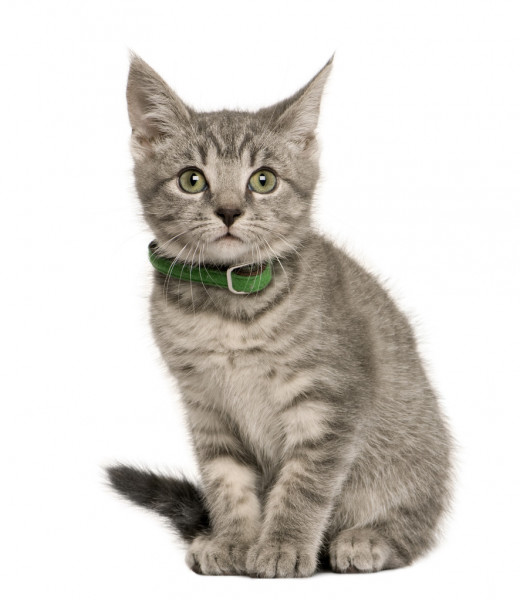
\includegraphics[width=\linewidth]{media/c1}
          \caption*{Anchor}\label{fig:cat1}
        \endminipage\hfill
        \minipage{0.32\textwidth}%
          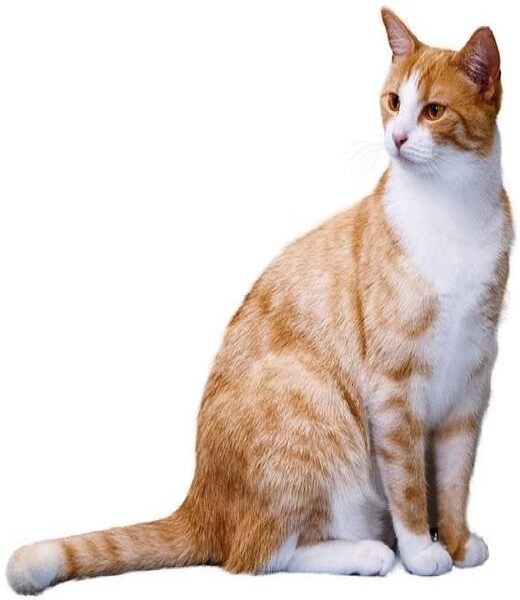
\includegraphics[width=\linewidth]{media/c2}
          \caption*{Positive example}\label{fig:c2}
        \endminipage
        \minipage{0.32\textwidth}%
          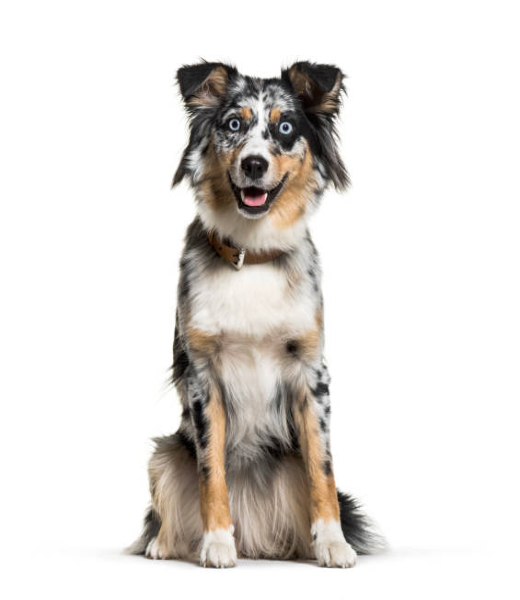
\includegraphics[width=\linewidth]{media/doggo}
          \caption*{Negative example}\label{fig:doggo}
        \endminipage
        \caption{Example of an anchor $x$, a positive instance $\ps$ and a negative instance $\ns$. Images obtained from \emph{Google}.}
        \end{figure}
    \end{nexample}
    


The main idea is to learn a representation of $x$, say $g(x)$, such that the distance of the representation of the input is closer in distance to the representation of the positive sample $\ps$ than the representation of the negative sample $\ns$. Using the norm\footnotemark, we can formally express that as follows: 
$$
\norm{g(x) - g(\ps)}_2 \leq \norm{g(x) - g(\ns)}_2,
$$
for each triplet in the set.


%------------- Footnotemark
\footnotetext{A definition of the norm can be found on Appendix \ref{APPENDIX:A}, Definition \ref{def:norm}. }
%----------------------


Support-vector machines (SVMs) are supervised learning models used for classification or regression problems. They are one of the most robust prediction methods. They search for a hyperplane $h$ in high or infinite dimensional space that separates the data as much as possible, making use of \emph{support vectors}, the datapoints that are closest to the hyperplane. If the data is linearly separable, we can select two hyperplanes $h_1,h_2$ that are parallel to $h$ and making the distance from them to $h$ as large as possible. That region is called the \emph{margin}.

Coming back to our triplets problem, we also want to introduce a margin between the distances of the elements of the triplets, in order to separate positive examples from negative examples as much as possible. This way, we introduce a \emph{margin} term $\alpha$, rewriting our last equation as follows:
\[
\norm{g(x) - g(\ps)}_2 + \alpha < \norm{g(x) - g(\ns)}_2.
\]
Using this inequality, we can define a hinge loss function for each triplet in the set:
\begin{equation}\label{triplet:single:loss}
\ell^\alpha (x,\ps,\ns) = \max \left(0, \norm{g(x) - g(\ps)}_2^2 - \norm{g(x) - g(\ns)}_2^2 + \alpha\right).
\end{equation}
This loss has been defined for a single triplet. Now, we can define a global loss that accumulates the loss in Equation \eqref{triplet:single:loss} using all the triplets in set.

\begin{ndef}
Given a set of triplets, each containing an anchor, a positive example and a negative example, $\mathcal T = \{(x_i,\ps_i,\ns_i)\}_{i \in \Lambda}$, we define a triplet loss as follows:
\begin{equation}\label{triplet:sum:loss}
\mathcal L (x_i,\ps_i,\ns_i) = \sum_{i \in \Lambda} \ell^\alpha(x_i,\ps_i,\ns_i).
\end{equation}

\end{ndef}



We use this loss to train models in order to improve the representations obtained.It would be interesting to present the model non-trivial metric to the learning algorithm. When the representation $g$ improves, this is harder to do, and this results in slow convergence and expensive data sampling methods.

\section{Generalization of triplet losses and $N-$pairs loss}

In a single evaluation of the loss function over a triplet during the learning process, we are comparing one positive sample to one negative sample. In practice, after looping over sufficiently many triplets, we expect the distance between positive examples and negative examples to be maximized. However, this will surely be a slow process if our dataset has many examples and also, in each step we will be separating the positive element from the specific negative element to which we are comparing it in that evaluation. Thus, the technique might be unstable \citep{Sohn2016ImprovedDM}.

In order to fix this, a good idea would be to compare in each evaluation a positive sample with multiple negative samples, generalizing the case exposed before. This way, we would like the positive sample to increase its distance to \emph{all} of the negative samples at the same time. Let us present a loss that generalizes the loss in Equation \eqref{triplet:sum:loss}.

\begin{ndef}
Let $\ps$ be a positive example of the anchor $x$, and consider the set $X^- = \{\ns_1,\cdots,\ns_{N-1}\}$ of $(N-1)$ negative samples. Given an encoder $g$, the $(N+1)-$tuplet loss is defined as follows:
\begin{equation}\label{nplus1:tuplet:loss}
\mathcal L_{(N+1)-\text{tuplet}}(x,\ps,X^-) = \log \left( 1+ \sum_{i=1}^{N-1} \exp \left(g(x)^T g(\ns_i) - g(x)^T g(\ps)\right)\right) 
\end{equation}
\end{ndef}

\begin{remark}
If we consider the case $N=2$, we have
\[
\mathcal L_{(2+1)-\text{tuplet}}(x,\ps,\ns) = \log \left( 1+ \exp \left(g(x)^Tg(\ns) - g(x)^T g(\ps)\right)\right).
\]
This expression is very similar to the one in Equation \eqref{triplet:single:loss}. In fact, if the norm in Equation \eqref{triplet:single:loss} is unit and $g$ minimizes $\mathcal L_{(2+1)-\text{tuplet}}$, then it minimizes $\ell^\alpha$, and hence both losses are equivalent.
\end{remark}



Applying the $(N+1)-$tuplet loss in deep metric learning is computationally expensive. Indeed, if we apply Stochastic Gradient Descent (SGD) with batch size $M$, then we have to evaluate $M \times (N+1)$ times our function $\ell^\alpha$ in each update. Because of this, if we increase $M$ and $N$, the number of evaluations grows quadratically. We would like to avoid this.

Consider the set of $N$ \emph{pairs} of examples, with the constraint of each pair belonging to a different class, i.e. $X = \{(x_1,\ps_1),\cdots,(x_N,\ps_N)\}$ with $y_i \neq y_j$ for all $i \neq j$. We now build $N$ tuplets where each tuplet has all the positive samples and the $i-th$ anchor, that is:
\[
\{S_i\}_{i=1}^N, \quad \text{where} \quad S_i = \{x_i, \ps_1,\cdots,\ps_N\}.  
\]
We can consider that each tuplet has $x_i$ as anchor, $\ps_i$ as positive example and $\ps_j$ for $j \neq i$ as negative samples, since they were all from different classes.

\begin{ndef}
In the last conditions, we can define the \emph{multi class N-pair loss} as follows:
\begin{align}
\mathcal L_{N-pair-mc} & \left(\left\{(x_i,\ps_i)\right\}_{i=1}^N \right)  = \nonumber \\
& \frac{1}{N} \sum_{i=1}^N \log \left(1+ \sum_{j\neq i} \exp\left(g(x_i)^T g(\ps_j) - g(x_i)^Tg(\ps_i)\right)\right) \label{N:Pair:loss}
\end{align}
\end{ndef}
This way, we are combining the $(N+1)-$tuplet loss and the $N-$pair construction that we presented, enabling highly scalable training. This loss has empirically proved in to have advantages if we compare it to other variations of mini-batch methods \citep{Sohn2016ImprovedDM}.

\subsection{InfoNCE Bound as a triplet loss}

The InfoNCE loss on Equation \eqref{NCE:loss} has proved to be useful in representation learning. Let us consider a reformulation on it. Firstly, since $f_k$ was an exponential, we can also consider $e^f$ and remove the exponential from $f$, this is just notation. Now, in \cite{poole_variational_2019} the InfoNCE bound in \eqref{Bound:NCE} is rewritten as follows:
\[
I(X,Y) \geq E\left[ \frac{1}{N} \sum_{i = 1}^N \log \frac{e^{f(x_i,y_i)}}{\frac{1}{N}\sum_{j=1}^N e^{f(x_i,y_j)}}\right] \triangleq  I_{NCE}(X,Y)
\]
where we have just named the right hand side of the inequality as $I_{NCE}(X,Y)$. Now, we can transform it in the following way:
\begin{align}
I_{NCE}  & = E\left[ \frac{1}{N} \sum_{i = 1}^N \log \frac{e^{f(x_i,y_i)}}{\frac{1}{N}\sum_{j=1}^N e^{f(x_i,y_j)}}\right]\nonumber \\
& = E\left[ \frac{1}{N} \sum_{i = 1}^N \log \frac{1}{\frac{1}{N}\sum_{j=1}^N e^{f(x_i,y_j) - f(x_i,y_i)}}\right]\nonumber \\
& = E\left[ -  \frac{1}{N} \sum_{i = 1}^N \log \frac{1}{N} \sum_{j=1}^N e^{f(x_i,y_j) - f(x_i,y_i)}\right] \label{last:eq:INCE}
\end{align}
And now, we only have to use the basic properties of the logarithm to see that
\begin{align}
\text{\eqref{last:eq:INCE}} & = E\left[-\frac{1}{N}\left(\sum_{i=1}^N \log \frac{1}{N} + \sum_{i=1}^N \log \sum_{j = 1}^N e^{f(x_i,y_j) - f(x_i,y_i)} \right)\right] \nonumber \\
& = E\left[-\frac{1}{N}\left( N(\cancel{\log 1} - \log N ) + \sum_{i=1}^N \log \left( 1  + \sum_{j \neq i} e^{f(x_i,y_j) - f(x_i,y_i)} \right)\right)\right] \nonumber\\ 
& = E\left[-\frac{1}{N}\left(-N\log N\right)\right] + E\left[-\frac{1}{N}\sum_{i=1}^N \log \left( 1  + \sum_{j \neq i} e^{f(x_i,y_j) - f(x_i,y_i)} \right)\right] \nonumber \\
& = \log N - E\left[ \frac{1}{N} \sum_{i=1}^N \log \left( 1+ \sum_{j\neq i}e^{f(x_i,y_j)- f(x_i,y_i)}\right)\right] \label{final:form:INCE}
\end{align}

In the particular case where $X,Y$ take values in the same space and $f$ has the particular form 
\[
f(x,y) = \phi(x)^T \phi(y),  
\]
for some $\phi$, Equation \eqref{final:form:INCE} is the same (up to constants and change of sign) as the expectation of the multi-class $N-$pair loss in Equation \eqref{N:Pair:loss}.

Hence, we have found an equivalence between representation learning by maximizing $I_{NCE}$ using a symmetric separable critic $f(x,y)$ and an encoder $g$ shared across views and using a multi class $N-$pair loss, which is a generalization of a triplet loss.



\clearpage

\ctparttext{
  \color{black}
  \begin{center}
  In this part, deep learning and neural networks will first be motivated and later be presented. Then, the two most important frameworks that use contrastive learning for representation learning will be completely explained.
  \end{center}
}
\part{New Frameworks for Representation Learning}
\chapter{SimCLR}
\label{Chapter:SimCLR}
\section{Introduction}

Until this point of the work, we have been presenting the theoretical basis of representation learning using contrastive learning. Previous approaches, such as  the framework presented in \cite{oord_representation_2019}, use a generative approach as a part of the representation learning process. Although this can be beneficial at some points and, in fact, achieved the \emph{state-of-art}\footnotemark empirical results, we have to consider that generative models have some drawbacks. 

%------------- Footnotemark
\footnotetext{\emph{State-of-art} refers to the best results that have been achieved at some point of time.}
%----------------------


Let us set in the case of learning representations of images to present a very simple example. In this case, generative models must \emph{generate} each pixel on the image. This can be extremely computationally expensive. 

Until now, we had been trying to minimize the loss in Equation \eqref{NCE:loss}, which we proved that maximizes a lower bound in the mutual information. However, some papers such as \cite{chen_simple_2020}, \cite{tschannen_mutual_2020}, suggest that it is unclear if the success of their methods is caused by the maximization of mutual information between the latent representations, or by the specific form that the constrastive loss has.

In fact, in \cite{tschannen_mutual_2020} they provide empirical proof for the loose connection between the success of the methods that use MI maximization and the utility of the MI maximization in practice. They also empirically proof  that the encoder architecture can be more important than the estimator used to determine the MI.

Even with the empirically proved disconnection between MI maximization and representation quality, recent works that have used the loss function defined in Equation \eqref{NCE:loss} have obtained state-of-art results in practice. 

Both SimCLR and BYOL (the framework that we will present later), are examples of \emph{siamese neural networks}. We remark it as a definition since it is important for the later explanation.

\begin{ndef}
A \emph{siamese neural network} is a type of NN architecture that contains (typically) two NNs which have the same configuration, parameters and weights. The parameters are updated the same way across both networks. 
\end{ndef}

These networks are usually used to find the similarity between the inputs by comparing produced feature vectors. They are more robust to class imbalance, nice to an ensemble with the best classifier (since the classifier is built on top of the representation extractors), and learn from semantic similarity.


\section{SimCLR framework}

\emph{SimCLR} \citep{chen_simple_2020} presents a framework that achieved state-of-art results when it was presented in July 2020. It also uses contrastive learning in an specific way that we will present later. 

This framework learns representations by maximizing agreement between examples of the same input obtained by using data augmentation on the input example and a contrastive loss in the latent space. 


\begin{figure}[H]
    \small
        \centering
    \begin{tikzpicture}
        \node at (0,1.8) (h) {$\longleftarrow\,$Representation$\,\longrightarrow$};
        \node[draw, circle] at (0,-1) (x) {$\,~\bm{x}~\,$};
        \node[draw, circle] at (-2.5,0) (x1) {$\tilde{\bm{x}}_i$};
        \node[draw, circle] at (2.5,0) (x2) {$\tilde{\bm{x}}_j$};
        \node at (-2.5,1.8) (h) {$\bm h_i$};
        \node at (2.5,1.8) (c) {$\bm h_j$};
        \node at (-2.5,3) (hh) {$\bm z_i$};
        \node at (2.5,3) (cc) {$\bm z_j$};
        \path[->] 
            (x)  edge [>=latex] node[below,rotate=-25] {$t\sim\mathcal{T}$} (x1)
            (x)  edge [>=latex] node[below,rotate=25] {$t'\sim \mathcal{T}$} (x2)
            (x1)  edge [>=latex] node[left,rotate=0] {$f(\cdot)$} (h)
            (x2)  edge [>=latex] node[right,rotate=0] {$f(\cdot)$} (c)
            (h)  edge [>=latex] node[left,rotate=0] {$g(\cdot)$} (hh)
            (c)  edge [>=latex] node[right,rotate=0] {$g(\cdot)$} (cc);
        \path[<->]
            (hh)  edge [>=latex] node[above,rotate=0] {Maximize agreement} (cc);
        \end{tikzpicture}
        \caption{Figure obtained from \cite{chen_simple_2020}. A simple framework for contrastive learning of visual representations.}
        \label{fig:framework:SimCLR}
    \end{figure}


The framework that is presented follows a linear structure. Figure \ref{fig:framework:SimCLR} depicts it. Let us provide with deeper explanation. We will present the steps in a general way and later we will remark the specific considerations that were used in the implementation of the framework for the experiments. 

The steps followed are:
\begin{enumerate}
\item Firstly, using the input $x$ and two augmentation functions $t,t' \in \mathcal T$, two different views $\tilde x_i,\tilde x_j$ are obtained using data augmentation. They are both sampled from the same family of data augmentations $\mathcal T$. They are \emph{both} considered as positive views.
\item Secondly, a NN base encoder $f(\cdot)$ is used to extract representations for the two different views, obtaining $h_i = f(\tilde{x_i})$, where $h_i \in \R^d$.  

\item Then, a \emph{small} neural network projection $g(\cdot)$ is used. This neural network maps the representations $h_i$ to the space where contrastive loss is applied. Hence, we obtain 
$$
z_i = g(h_i) = W^{(2)}\sigma(W^{(1)}h_i),$$
where $\sigma$ is a nonlinear function and $W^{(i)}$ are the weights matrix.

\item Lastly, the contrastive loss is used for a contrastive prediction task. Using a set $\{\tilde x_k \}$ that includes a pair of positive examples $\tilde x_i,\tilde x_j$, the contrastive loss will (as we have already been doing theoretically) try to identify $\tilde x_j$ in the set for a given $\tilde x_i$. It is important to remark how the contrastive loss is used in this framework:
\begin{enumerate}
\item A minibatch of $N$ samples is randomly taken from the training set. 
\item Using the $N$ samples, we augment each pair to obtain $2N$ data points. The idea is, given a positive pair, use the other $2(N-1)$ as negative examples.
\item We define
\[
sim(u,v) = \frac{u^T v}{\norm{u}\norm{v}},    
\]
the normalized dot product between $u$ and $v$. This function is also known as the \emph{cosine similarity}. Then, the loss function for a positive pair of examples takes the form:
\begin{equation}\label{c:loss:simclr:ind}
\ell_{i,j} = -\log \frac{exp(sim(z_i,z_j)/\tau)}{\sum_{k=1}^{2N} \mathbb{1}_{k \neq i} exp(sim(z_i,z_k)/\tau)},    
\end{equation}
where $\mathbb{1}_{k \neq i} \in \{0,1\}$ produces $0$ if $k = i$ and $1$ elsewhere. $\tau$ is a temperature parameter that has to be adjusted.
\item The final loss is computed across all the positive pairs, both $(i,j)$ and $(j,i)$ in the minibatch.
\begin{equation}\label{c:loss:simclr}
\mathcal L = \frac{1}{2N} \sum_{k=1}^{2N} \left(\ell(2k-1,2k) + \ell(2k,2k-1)\right).
\end{equation}
\end{enumerate}
\end{enumerate}
\begin{remark}
The loss in Equation \eqref{c:loss:simclr} is just another formulation of the one in Equation \eqref{NCE:loss}, applied to this particular way of obtaining positive and negative views.
\end{remark}

We can summarize all this steps in the following algorithm:
\begin{figure}[H]
\begin{algorithm}[H]
    \caption{\label{alg:main} SimCLR's learning algorithm.}
    \begin{algorithmic}
        \STATE \textbf{input:} batch size $N$, temperature $\tau$, structure of $f$, $g$, $\mathcal{T}$.
        \FOR{sampled minibatch $\{\bm x_k\}_{k=1}^N$}
        \STATE \textbf{for all} $k\in \{1, \ldots, N\}$ \textbf{do}
            \STATE $~~~~$draw two augmentation functions $t \!\sim\! \mathcal{T}$, $t' \!\sim\! \mathcal{T}$
            \STATE $~~~~$\textcolor{gray}{\# use augmentations} 
            \STATE $~~~~$$\tilde{\bm x}_{2k-1} = t(\bm x_k)$
            \STATE $~~~~$$\tilde{\bm x}_{2k} = t'(\bm x_k)$
            \STATE $~~~~$\textcolor{gray}{\# use $f$} 
            \STATE $~~~~$$\bm h_{2k-1} = f(\tilde{\bm x}_{2k-1})$  \textcolor{gray}{~~~~~~~~~~~~~~~~~~~~~~~~~~~~~~\# representation}
            \STATE $~~~~$$\bm h_{2k} = f(\tilde{\bm x}_{2k})$      \textcolor{gray}{~~~~~~~~~~~~~~~~~~~~~~~~~~~~~~~~~~~~~~\# representation}
            \STATE $~~~~$\textcolor{gray}{\# use $g$} 
            \STATE $~~~~$$\bm z_{2k-1} = g({\bm h}_{2k-1})$  \textcolor{gray}{~~~~~~~~~~~~~~~~~~~~~~~~~~~~~~~~\# projection}
            \STATE $~~~~$$\bm z_{2k} = g({\bm h}_{2k})$      \textcolor{gray}{~~~~~~~~~~~~~~~~~~~~~~~~~~~~~~~~~~~~~~~~\# projection}
        \STATE \textbf{end for}
        \STATE \textbf{for all} $i\in\{1, \ldots, 2N\}$ and $j\in\{1, \dots, 2N\}$ \textbf{do}
        \STATE $~~~~$ $s_{i,j} = \bm z_i^\top \bm z_j / (\lVert\bm z_i\rVert \lVert\bm z_j\rVert)$ \textcolor{gray}{~~~~~~~~\# compute similarity}\\
        \STATE \textbf{end for}
        \STATE update networks $f$ and $g$ to minimize $\mathcal{L}$ defined in Eq. \eqref{c:loss:simclr}
        \ENDFOR
        \STATE \textbf{return} encoder network $f(\cdot)$, and throw away $g(\cdot)$
    \end{algorithmic}
    \end{algorithm}
    
    \caption{Algorithm that summarizes the learning process that SimCLR follows.}
\end{figure}

Considerations:
\begin{enumerate}
\item In SimCLR, the data augmentation is applied sequentially, and using three techniques of image data augmentation that are very simple and common:
\begin{enumerate}
\item Random cropping followed by resize to original size,
\item Random color distortions, which consist of changing the value of certain amount of pixels randomly, like color jittering or changing from colored images to black and white images.
\item Random Gaussian Blur: Gaussian Blur consists of convolving an image with a \emph{Gaussian function}.
\end{enumerate}

\item For the base encoder $f(\cdot)$, a \emph{ResNet} network is used because of its simplicity.
\item For the projection head $g(\cdot)$, a MLP with one hidden layer is used, and \emph{ReLU} is used as the activation function $\sigma$.
\end{enumerate}



\section{Findings of SimCLR}

    Using the algorithm structure that we have presented, the experiments focused on finding what made the biggest impact on the representation learning task. 
    
    Intuitively, since we are comparing $2N$ images, either positive or negative, the batch size that we will use for the experiment should be as big as possible. Comparing a positive sample and trying to push it apart from as much negative samples as possible in the same iteration sounds like a good idea for the quality of our representations.
    
    
    A few of the most relevant findings using SimCLR are: 
    \begin{itemize}
    \item In the SimCLR framework, multiple data augmentations are used and it is empirically shown that this improves the contrastive prediction tasks that yield effective representations.
    
    \item The introduction of a nonlinear transformation that it can be learnt during the learning process. This linear transformation is between the representation and the contrastive loss, so before evaluating the loss function, the representation is applied the nonlinear function.
    
    \item The contrastive loss benefits from normalized embeddings and also from a temperature parameter that has to be adjusted.
    
    \item This loss also benefits from larger batch sizes and longer training, as well as from deeper and wider networks.
\end{itemize}

Later, \emph{SimCLRv2} was presented \citep{chen2020big}, achieving a new state-of-art in semi-supervised learning on the ImageNet dataset. In this new framework, semi-supervised learning is use . This approach involves unsupervised learning followed by supervised fine-tuning\footnotemark. After this stages that are similar to SimCLR,  a final stage is added. It consists of \emph{distillation} with unlabeled examples for refining the task-specific knowledge.


In the self-supervised (or unsupervised) part, the images are used without its labels, so that the representations of them that are obtained by the framework are not related to an specific task. Using this technique, \cite{chen2020big} shows how using deeper and wider neural networks for both self-supervised pretraining and fine-tuning improves accuracy greatly. Also, the importance of the projection head $g(\cdot)$ is remarked in this new framework.
%------------- Footnotemark
\footnotetext{\emph{Fine-Tuning} refers to the process of re-training certain parts of an already trained NN so that it focuses its learn on specific examples, such as a different dataset.}
%----------------------
\chapter{Boostrap Your Own Latent}
\label{Chapter:BYOL}

\section{Motivation}

We have shown how contrastive methods rely on comparing different views of the same image with views of other images, considering the ones from the same image as positive and the rest as negative samples. This is why they are called \emph{self-supervised} methods.

Self-supervised methods build upon the cross-view prediction framework, i.e., learning representations by predicting different views (or data augmentations) of the same image. This could lead the frameworks to collapsed representations, such as a constant representation for any view of the image can easily help us to identify objects, but it is useless for downstream tasks.

The methods presented earlier, which use contrastive learning, avoid this problem by trying to discriminate between positive and negative views, as we have already explained.

However, some papers (e.g. \cite{caron2019deep}) have already raised the following question:

\begin{quote}
    \centering
\emph{ Is the use of negative samples necessary to avoid collapsing? }. 
\end{quote}
This question is studied in \cite{grill2020bootstrap}, paper that presents an algorithm that we will be deeply explaining.

The first solution that comes to mind to prevent the collapsing problem would be to use a randomly initialized network to produce the targets of the predictions. As it is probably expected, due to its randomness, it does not produce good representations for downstream tasks. Nonetheless, the representations obtained were empirically much better than initial fixed representation, so it could be interesting to refine this representation in order to make it better for the later tasks. This is the intuitive idea behind \emph{Boostrap your own latent (BYOL)} \citep{grill2020bootstrap}.

\section{BYOL Algorithm}

BYOL's algorithm has certain similarities with the SimCLR framework that we presented in Chapter \ref{Chapter:SimCLR}. The goal of this framework is to learn a representation for an input. In this case, the representation will be noted as $y_\theta$. 

For this purpose, two neural networks are used:
\begin{itemize}
\item An \emph{online} network defined by a set of weights $\theta$.

\item A \emph{target} network, defined by a different set of weights $\upxi$.
\end{itemize}

They both have the same structure, composed of three stages:
\begin{enumerate}
\item An encoder $f_\gamma$,
\item A projector $g_\gamma$,
\item A predictor $q_\gamma$,
\end{enumerate}
where $\gamma \in \{\theta,\upxi\}$. In the online network, despite their different name, the projector $g_\theta$ and the predictor $q_\theta$ have the same architecture.

\begin{remark}
The projector $g_\gamma$ is used because in SimCLR \citep{chen_simple_2020} is proven empirically that this projection improves the general performance of the framework.
\end{remark}

The \emph{difference} between them is that the target network provides the regression targets to train the online network, and its parameters $\upxi$ are an exponential moving average\footnotemark of the online parameters $\theta$. Mathematically, given a rate decay $\tau \in [0,1]$, after each training step $\upxi$ is updated as follows:
\[
\upxi \leftarrow \tau \upxi + (1-\tau)\theta    
\]

%------------- Footnotemark
\footnotetext{A moving average is a calculation to analyze data points by creating a series of averages in different subsets of the data. }
%----------------------

Having presented the networks and its structure, the following steps are followed in BYOL's framework:

\begin{enumerate}
\item The input that both networks receive is different, even if it comes from the same image. As in SimCLR, given an input image $x$ and two distributions of data augmentation for images, $\mathcal T, \mathcal T'$, two views are produced from $x$ to get $v = t(x), v' = t'(x)$ where $t \sim \mathcal T $ and $t' \sim \mathcal T'$.

\item Each produced view is passed to one of the networks. In particular, the first view $v$ is passed to the online network, and follows the next steps:
\[
x \longmapsto v = t(x) \longmapsto y_\theta = f_\theta(v) \longmapsto z_\theta =  g_\theta(y_\theta)    
\]
where $f_\theta,g_\theta$ are the ones that we mentioned before in the structure of each networks. This online network outputs $y_\theta$ and $z_\theta$.

In a similar process, the the target network is passed the second view $v'$, which follows the next steps:
\[
x \longmapsto v' = t'(x) \longmapsto y_\upxi' = f_\upxi(v') \longmapsto z_\upxi' = g_\upxi(y_\upxi')   
\]
where, again, $f_\upxi,g_\upxi$ are the ones mentioned before.


\item Then, using the online network, a prediction $q_\theta(z_\theta)$ is produced. Remark that the prediction is \emph{only} applied to the online network.

\item Having $q_\theta(z_\theta)$ in the online network and $z_\upxi'$ in the target network, they are both $\ell_2$-normalized to
\[
\overline{q_\theta}(z_\theta) = \frac{q_\theta(z_\theta)}{\norm{q_\theta(z_\theta)}} \quad \text{and} \quad \overline{z_\upxi'} = \frac{z_\upxi'}{\norm{z_\upxi'}}. 
\]

\item \label{BYOL:not:last} Now, we can define the mean squared error between the normalized prediction $\overline{q_\theta}(z_\theta)$ and the normalized projection $\overline{z_\upxi'}$:
\[
\mathcal L_{\theta,\upxi} = \norm{\overline{q_\theta}(z_\theta) - \overline{z_\upxi'}}_2^2. 
\]

\item If we stopped in the step \ref{BYOL:not:last}, the framework would be asymmetric between the two networks, since the projection is performed in one of the views, $v$ but not in the other one, $v'$. To fix this, the process described is repeated except that now $v'$ is the input of the online network and $v$ is the input of the target network, producing a new loss $\tilde{\mathcal L}_{\theta,\upxi}$. The final loss is computed as:
\begin{equation}\label{Loss:BYOL}
\mathcal L_{\theta,\upxi}^{\operatorname{BYOL}}     = \mathcal L_{\theta,\upxi} + \tilde{\mathcal L}_{\theta,\upxi} 
\end{equation}
\end{enumerate}

The loss in Equation \eqref{Loss:BYOL} is the one that must be optimized stochastically. Furthermore, since we have expressed $\upxi$ depends on $\theta$, if $\eta$ is the learning rate that we want to apply, the optimization problem can be expressed as follows:
\[
\begin{cases}
    \theta \gets \operatorname{optimizer}\left(\theta,\nabla_\theta \mathcal L_{\theta,\upxi}^{\operatorname{BYOL}},\eta \right), \\
    \upxi \gets \tau \upxi + (1-\tau)\theta 
\end{cases}
\]

The framework can be summarized in the following figure:
\begin{figure}[H]
    \centering 
    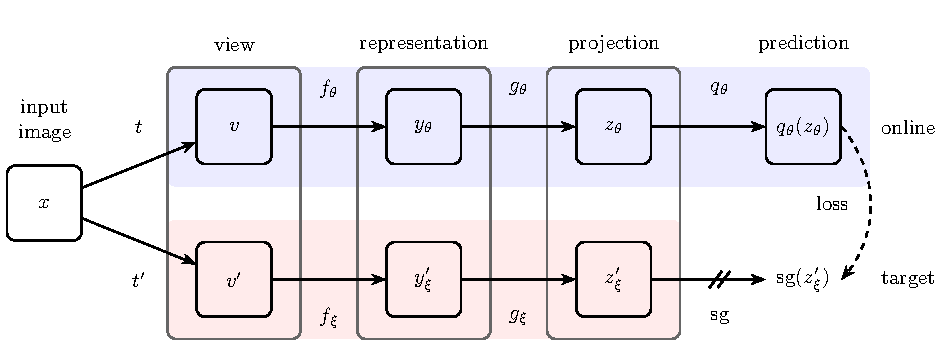
\includegraphics[scale=0.8]{Archi-BYOL.pdf}
    \caption{Image from \citep{grill2020bootstrap}. Overview of Bootstrap Your Own Latent Framework. }
\end{figure}

The \emph{sg (stop gradient)} indicates that, at that point, the gradient is not propagated back. 

After the whole model has been fully trained, both the projection $g_\theta$  and the prediction $q_\theta$ are discarded, since what it is interesting for us is the representation of the input, and it is what it will be used in downstream tasks.

Some considerations have to be made about this framework:
\begin{enumerate}
    \item About data augmentation: In BYOL,it is not important if the model learns about the histogram of the image, since we want ot keep any information captured by the target representation into its online network. In the original paper, it is empirically shown how BYOL is more robust to the choice of the image augmentations than SimCLR.

    \item Since the weights of the target network $\upxi$ depend on the weights of the online network $\theta$ by a parameter $\tau$, the first mentioned weights $\upxi$ represent a delayed and stable version of $\theta$. Actually, if the decay rate $\tau$ is $1$, we never update $\upxi$, and if $\tau = 0 $, then the weights of the target network are always being updated. This way, a trade-off is tablished between updating $\upxi$ too often or too slowly. Empirically, it has been shown that the most adequate values that yield to more stable results are $\tau \in [0.9,0.999]$.
\end{enumerate}

\section{Results obtained by this framework}

In this framework, the impact of the batch size varies respect to the importance that it had in SimCLR. In contrast with BYOL's framework, in SimCLR we were using negative samples in our network to learn how to produce the representations. Because of this, BYOL's is expected to be more robust to smaller batch sizes. 

It is empirically shown that the regularization of the weights is crutial in the self-supervised setting. The experiments in the paper showed that removing the weight decay regularization led to model divergence.


BYOL achieved the state-of-art performance results in the linear evaluation. This is, again, one of the most interesting parts since it helps us to evaluate how good the representations that our model create are.

\begin{table}[H]
    \label{table:best:first:simclr}
\centering
\begin{tabular}{llrrr}
Method & Architecture & Params & Top-1 & Top 5 \\ \hline
SimCLR & ResNet-50($2\times)$ & 94M & 74.2 & 92.0 \\
BYOL & ResNet-50($2\times)$ & 94M & \textbf{77.4} & \textbf{93.6} \\
SimCLR & ResNet-50($4\times)$ & 375M & 76.5& 93.2 \\
BYOL & ResNet-50($4\times)$ & 375M & \textbf{79.6}& \textbf{94.8} \\
\end{tabular}
\caption{Comparison between SimCLR and BYOL Top1 and Top5 accuracies using the same architectures on the ImageNet dataset.}
\end{table}

BYOL also outperformed other models such as \emph{MoCo} \citep{he2020momentum} and a second version of the Contrastive Predictive Coding framework \citep{hénaff2020dataefficient}, but they have not been included in the table since they are not deeply studied in this work.

\ctparttext{
  \color{black}
  \begin{center}
  In this last part, the frameworks that we have presented in the last part will be tested. We will train the models in a specific dataset and the results obtained will be compared with the results of the original papers.
  \end{center}
}
\part{Experiments}
\chapter{Introduction}
In this chapter, we will explain the fundamentals and technologies that have been used for the experimentation. We will focus on three main aspects:
\begin{enumerate}
\item The used dataset.
\item The used libraries for the development of the code.
\item Analysis of the code itself.
\item The used metrics to evaluate the obtained results.
\end{enumerate}

The idea of the experimentation part is to test and compare the frameworks that we have presented in Chapters \ref{Chapter:SimCLR} and \ref{Chapter:BYOL}. Their architectures have already been explained, and the original code for both backbones has not been done by me. 

This work will focus on testing how changing the training hyperparameters of the model affects the final results, since the original papers \cite{chen_simple_2020,grill2020bootstrap} already mention that using their structure, the results are affected by those hyperparameters, such as batch size, network depth or network width.

The implementations that have been used can be found in:
\begin{itemize}
\item SimCLR implementation: Official implementation from Google in \url{https://github.com/google-research/simclr/tree/master/tf2}

\item BYOL implementation: not official, found in \url{https://github.com/garder14/byol-tensorflow2}. 
\end{itemize}

Although there exists an official implementation of BYOL, non-official one has been chosen because it uses \emph{Tensorflow}, which makes the implementations easier to understand and modify, which we needed to do. Also, the idea is to make use of \emph{Tensorboard}, a Tensorflow utility that helps with visualization and graph generation of the training and final results.


\section{Hardware and basic libraries}

When running training experiments in DL, the used hardware is one of the most determining factors for the results obtained by the models. There are many reasons for this, such as the time spent on the training a model or the amount of  data that we can fit in the GPUs (which will be our case) or TPUs.

For the experiments of this project, the DECSAI\footnotemark department of the University of Granada generously provided us access to a server that has a few NVIDIA GeForce RTX 3090. This model of GPU is one of the best in the market, having a \emph{compute capability} of $8.6/10$, rated by the NVIDIA company. IT also has a memory of $24GB$, which allows us to experiment with relatively large batch sizes using a single GPU and not having to parallelize the experiment.

%------------- Footnotemark
\footnotetext{The DECSAI's website is \url{https://decsai.ugr.es/}.}
%----------------------


To be able to use this GPUs in our experiments, two basic libraries have to be installed in the server:
\begin{enumerate}
\item \lstinline{tensorflow-gpu}. This is a variant of the \lstinline{tensorflow} library that was developed for using GPUs while using tensorflow.
\item \lstinline{CUDA 11.4}. CUDA is a parallel computing platform and API created by NVIDIA which allows to use a CUDA-enabled GPU for general purpose processing. In other words, CUDA is needed to be able to use the GPU in our \lstinline{python} scripts.
\end{enumerate}

These two libraries, along with other packages that are needed for creating graphics (\lstinline{Matplotlib,Seaborn}) or computing metrics (\lstinline{sklearn}) are installed using a \lstinline{Conda} environment in our server's user.


\section{The dataset: CIFAR10}

The computational resources that we have for the experiment are limited. Due to this, we must fix a dataset that, having enough and representative examples, allows us to achieve feasible training time and successful results.

One of the ever most used dataset, which was also used in both SimCLR and BYOL papers, is CIFAR10 \citep{krizhevsky_learning_nodate}. This dataset will be used to test the overall performance of our representation learning methods.

CIFAR10 contains $60.000$ images divided in $10$ classes, where each class contains $10.000$ images. The size of the images is $32\times 32\times 3$, so the size of the images is not very large. This helps us to have faster trainings.

\begin{figure}[H]
    \centering 
    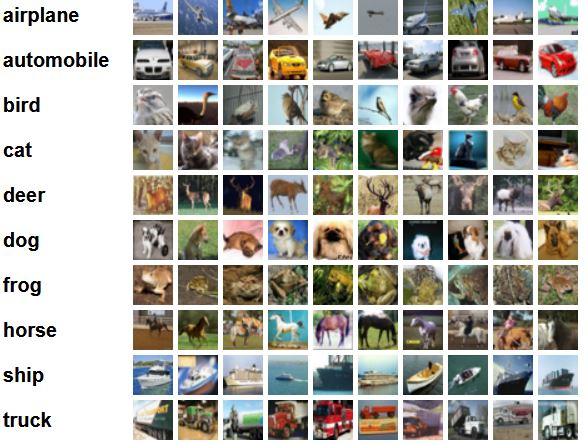
\includegraphics[scale=0.8]{CIFAR10}
    \caption{Ten examples of each class in the CIFAR10 dataset. }
\end{figure}
This dataset has $50.000$ samples for training and $10.000$ for test. The test batch contains the same number of examples of each of the $10.000$ classes in the dataset, that is, it contains $1.000$ examples of each class. 

It is important to remark that the classes are \emph{completely mutually exclusive}. That means that there is no overlap between the classes even if they have similar images, such as \emph{Cars} and \emph{Truck}, which are two of the classes of the dataset.

\section{Tensorflow}



Tensorflow\footnotemark is an open source library for developing machine learning frameworks.  

\begin{wrapfigure}{r}{5cm}
    \caption{Tensorflow logo.}
    
\includegraphics[scale=0.2]{tf-logo}
\end{wrapfigure}

%------------- Footnotemark
\footnotetext{Tensorflow documentation can be found at \url{https://www.tensorflow.org/}.}
%----------------------



It can be used for many tasks, but it focuses on training and inference of deep neural networks. It is used for both research and production at \emph{Google}, since it was also developed by the \emph{Google Brain} team for internal use. However, it was later released as open source.

The creation of new models is very simple, offering multiple abstraction levels. This is why it is suitable for our experiments. Also, the code is most of the times easily understandable.

There are other libraries that are widely used in machine learning algorithm development, such as \emph{PyTorch} or \emph{Jax}. However, Tensorflow has been chosen because I was a little bit more familiarized than with the other and because of its simplicity and how common it is. 

There are a few ways to define a NN or a framework using tensorflow. The most classic one is defining a sequential model using \lstinline{Keras}, a tensorflow API that defines layers of a neural network and helps with the implementation of simple NN structures. Let us see how to implement a very simple example of a NN with three \emph{Dense} layers: 

\begin{minted}[mathescape,linenos]{python}
model = keras.Sequential(
    [
        layers.Dense(2, activation="relu", name="layer1"),
        layers.Dense(3, activation="relu", name="layer2"),
        layers.Dense(4, name="layer3"),
    ]
)
\end{minted}

Another way of creating models using tensorflow is by defining a single step of training using \lstinline{tf.GradientTape()} and then executing the single step multiple times in a loop. Using GradientTape , tensorflow performs automatic differentiation, which is needed for the minimization process. Let us see the simplest example, consider the function $f(x) = x^2$, and imagine that we want to obtain $f'(3)$. We can obtain it using \lstinline{tf.GradientTape()} as follows:

\begin{minted}[mathescape,linenos]{python}
x = tf.constant(3.0)
with tf.GradientTape() as g:
  g.watch(x)
  y = x * x
dy_dx = g.gradient(y, x)
\end{minted}

In our case, the gradient is obtained and the applied to the optimizer by using:

\begin{minted}[mathescape,linenos]{python}
with tf.GradientTape() as tape:
    grads = tape.gradient(loss, model.trainable_variables)
    optimizer.apply_gradients(zip(grads, model.trainable_variables))
\end{minted}


\subsection{Tensorboard}

Tensorboard is a Tensorflow's visualization kit. It provides the visualization and tooling needed for machine learning experimentation. Among its more important utilities, we can find:
\begin{itemize}
\item Tracking and visualizing metrics (such as loss, accuracy, entropy) not only during the training but also when the training time has ended.

\item Visualizing the model graph: ops and layers.

\item Visualizing histograms of weights, biases and how tensors change during the training.

\item Projecting high-dimensional data to a lower dimensional space.

\item Displaying images,text and audio data.
\end{itemize}

Also, it is very easy to integrate with tensorflow.  Actually, in most of the cases it is as simple as adding the following \emph{callback} when we fit the model:

\begin{minted}[mathescape,linenos]{python}
    tensorboard_callback = tf.keras.callbacks.TensorBoard
                        (log_dir=log_dir, histogram_freq=1)
    model.fit(x=x_train, y=y_train, 
              epochs=5, 
              validation_data=(x_test, y_test),
              # The added callback produces the magic! 
              callbacks=[tensorboard_callback])  
\end{minted}

In our case, there are some differences, since we are not using the standard \lstinline{fit} function to train our models. Because of this, we have to log the information that we have obtained in each step. To do this, we can use the \lstinline{metrics} python package to group them (as it is done in the SimCLR code), or we can just directly save the information creating a \emph{file writer} and writing the desired variables on this file. We do this in the modification that we have done to BYOL's original code as follows:

\begin{minted}[mathescape,linenos]{python}
train_summary_writer = tf.summary.create_file_writer(args.log_dir)
with train_summary_writer.as_default():
    tf.summary.scalar('top_1_acc',float(acc),step=epoch)
    tf.summary.scalar('top_5_acc',float(top_5_acc),step=epoch)
    tf.summary.scalar('loss', float(losses[-1]), step=epoch)
\end{minted}


\section{Metrics}

As we have seen, firstly, our models create a representation of the input image and then this representation is evaluated using a supervised linear head. This is the most interesting part, since we can see if the representation obtained was really useful for the classification task. We need to present the measures that we will use to measure how good the representations that we are producing are.



\begin{notation}
We will address the \emph{true positives} (the positive samples of a class classified correctly) as $TP$, the \emph{true negatives} (the negative samples classified correctly) as $TN$, the \emph{false positives} (the negative samples classified as positive ones, which is a mistake of our model) as $FP$ and the false negatives (the positive samples classified incorrectly as negative samples) as $FN$.
\end{notation}

Using this notation, the measures that we will be using are the following:

\begin{itemize}
\item \emph{Accuracy}. The classic measure for models. It measures the number of successes our network has obtained producing the correct label for the representation created during the unsupervised part of the network. Formally,
\[
\operatorname{Accuracy} = \frac{TP + TN}{TP + TN + FP + FN}  .  
\] 
In SimCLR, we wil use two kinds of accuracies:
\begin{enumerate}
\item \emph{Top1} accuracy, which is the ordinary accuracy.
\item \emph{Top5} accuracy, which measures if any of the 5 highest probability answers matches the true label.
\end{enumerate}
\end{itemize}





\chapter{Experimentation}
We are now ready to perform the experiments. We will begin exploring SimCLR implementation and results, later we will explore BYOL's implementation and lastly we will compare them in order to see how BYOL tries to improve SimCLR and we will check if it successess or not.

The code used for the experimentations, as well as some files with the results, can be found on the Github repository for this work.

\section{SimCLR exploration}
We will perform an iterative exploration with this framework. We will explore a few range for a subset of the hyperparameters and then we will go deeper into some hyperparameters to try and obtain better results.

\subsection{First approach}
\label{experiments:simclr:first}

The first thing we did to experiment with this framework is to explore a wide range of hyperparameters to see which set of them performed better for us. The script that can be found in \lstinline{code/SimCLR/run.py}.

What we did for this first exploration was to define a \emph{parameter grid} and execute the whole framework using each combination of the parameters. The parameters that were firstly considerered are:
\begin{enumerate}
\item \lstinline{batch_size}. This is one of the most important parameters of SimCLR. In the original paper, it was proven that the higher this parameter, the better the results obtained for the linear classification. This parameter is also important since it has to adapt to our GPU's memory. The options that we have considered for the first experiments are: \lstinline|batch_size = {512,1024}|.

\item \lstinline{temperature}. The temperature parameter $\tau$ plays an important role in the individual loss seen in Equation \eqref{c:loss:simclr:ind}. It is suggested to try values in the range $[0,1]$ and the one that had better performance for the original experiments was around $0.5$, so we chose the following values: \lstinline|temperature = {0.25,0.5,0.75,1}|.

\item \lstinline{color_jitter_strength}. This parameter measures how hard is the color variation in the data augmentation. Previous results show that this parameter is important for the success of the network, so we provide with a big range of values. We include the following values: \lstinline|color_jitter_strength = {0.25,0.5,0.75,1}|.
\end{enumerate}

Using python and the python function \lstinline{itertools.product} we straightforwardly generate all possible different combinations of unions of the parameters so we only have to append them to a general string and execute the \lstinline{run.py} script mentioned before to obtain the results. In total, we obtain $32$ possible combinations, so we will obtain $32$ models. 

The script was executed and took approximately $24$ hours to train and evaluate all the different models, obtaining the results in Table \ref{table:simclr:gridsearch:1} in Appendix \ref{APPENDIX:B}. We have to remark, for each of the two possible batch sizes, the best results obtained. These are:

\begin{table}[H]
    \label{table:best:first:simclr}
\centering
\resizebox{\columnwidth}{!}{
\begin{tabular}{rrrrrrr}
batch\_size   & temperature   & color\_jitter & regularization\_loss & top\_1\_accuracy & top\_5\_accuracy & steps         \\ \hline
 512  &  0.25 &  0.25 &  0.0093      &  0.833         &  0.994          &  9800 \\
 1024 &    0.25       &  0.75 &  0.0093      &  \textbf{0.841}          &  0.995          &  4900 \\
\end{tabular}
}
\caption{Best results for the grid search experiment with SimCLR.}
\end{table}

\begin{remark}
On the original paper, the Top 1 accuracy score reported for CIFAR10 in $100$ epochs was $\sim 84.6\%$ accuracy for batch size $512$ and $\sim 85.1 \%$ accuracy score for $1024$ batch size. If we have a look at the results obtained in our experiment, we can say that our first attempt was \emph{successfull}.
\end{remark}

Let us make some observations. The clearest is that, since the second batch size doubles the first one, the training ends in half the steps. We can see that the temperature obtained in both cases is the same, and it is equal to $0.25$. However, there is a big change in the color jitter parameter: while using $512$ as batch size obtains the best result with the value of $0.25$ for color jitter, using $1024$ as batch size this value changes to $0.75$, which implies stronger color changes on the data augmentation. 

In general, having a look again at the Table \ref{table:simclr:gridsearch:1} in Appendix \ref{APPENDIX:B},  we can see that:

\begin{itemize}
    \item As it also happens in the experiments made on the original SimCLR paper, lower temperature $\tau$ parameters cause higher accuracies on the linear heads of our models.
    
    \item The models perform better when the \lstinline{color_jitter} parameter is in the range $[0.5,0.75]$. This means that, in general, a generous amount of color jittering to our picture is benefitial for the models.

    \item The \emph{Top 5 accuracy} is above $99\%$ in each model. This says that, since the models almost always give the correct label one of the 5 highest values, but they obtain the correct tag around $84\%$ of the times, they might be creating some similar representations of the data for inputs that do not belong to the same class. 
\end{itemize}

\subsection*{Observations about the batch size}

Although both models get to the same value of regularization loss, the model with a batch size of $1024$ obtains a higher \emph{top 1 accuracy}. This seems to follow the intuitive idea that we presented before: SimCLR benefits from bigger batch sizes since it allows a positive sample to be compared and pushed appart from negative samples. Ideally, we would keep pushing the batch size parameter forward, doubling it again to try to find out if the performance of the model keeps benefiting from bigger batch sizes. However, this requires either using multiple GPUs(or TPUs) working in parallel on the training or using GPUs with bigger memory, which we do not have access to. 

Using the resources we have, the following experiment was performed: using the hyperparameters that we found out in our \emph{GridSearch} to be the ones that achieve the best results except for the \lstinline{batch-size}, we train models moving the batch size in the following range: 
$$
\text{\lstinline{batch-size}}=\{16,32,64,128,256,512,1024\},
$$
where the last two values had already been computed in the GridSearch so we do not have to repeat the training.

\begin{figure}[htp] 
    \centering
    \subfloat[Evolution of the Top 1 accuracy with the batch size.]{%
        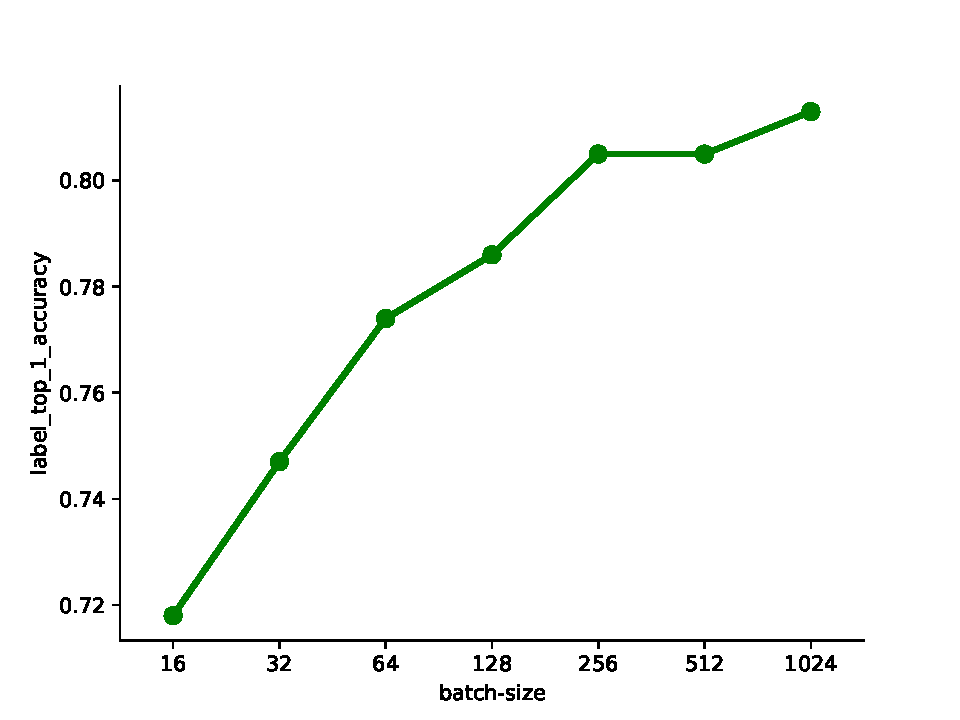
\includegraphics[width=0.45\textwidth]{simclr-batch-comparison}%
        \label{fig:accs:per:batch:simclr}%
        }%
    \hfill%
    \subfloat[Evolution curves of the accuracy with the steps taken in the training.]{%
        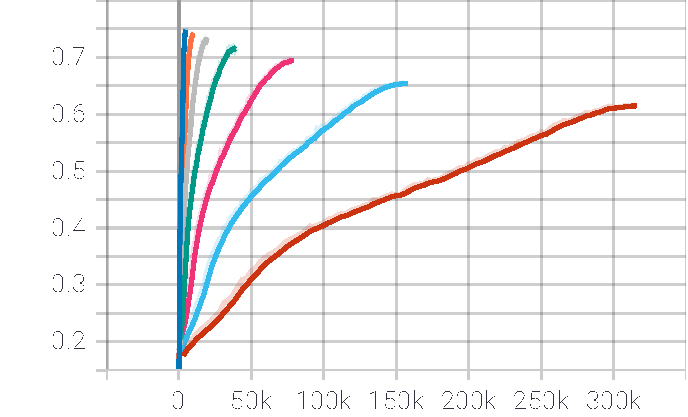
\includegraphics[width=0.45\textwidth]{train_supervised_acc}%
        \label{fig:evolution:acc:batches:simclr}%

        }%
        \caption{Results of the batch-size experiment.}
\end{figure}

Figure \ref{fig:accs:per:batch:simclr} shows the clear improvement of the Top 1 accuracy score when increasing the size of the batch that is used to compute the loss of our model. Increasing from $16$ to $1024$ gives an increase of more than $8\%$ in Top 1 accuracy, which is a lot. Further increase can be obtained if we keep increasing the batch size, but this is beyond our computation possibilities.

Figure \ref{fig:evolution:acc:batches:simclr} supports what we have just presented: not only with a smaller batch size we have to do thousands of extra steps in the training, but also we obtain much better accuracy performance of the linear head of the model.

\subsection*{Observations ofher hyperparameters}

We have seen that in our first experiment, batch size has been really relevant in the final results. We would like to see if the rest of the parameters play such an important role as well. 

As we have seen before, the parameters that we want to see how they affect the models are the \lstinline{color_jitter_strength} and the \lstinline{temperature} $\tau$ parameter. Let us study their impact on the model one by one. 

\begin{figure}[H] 
    \centering
    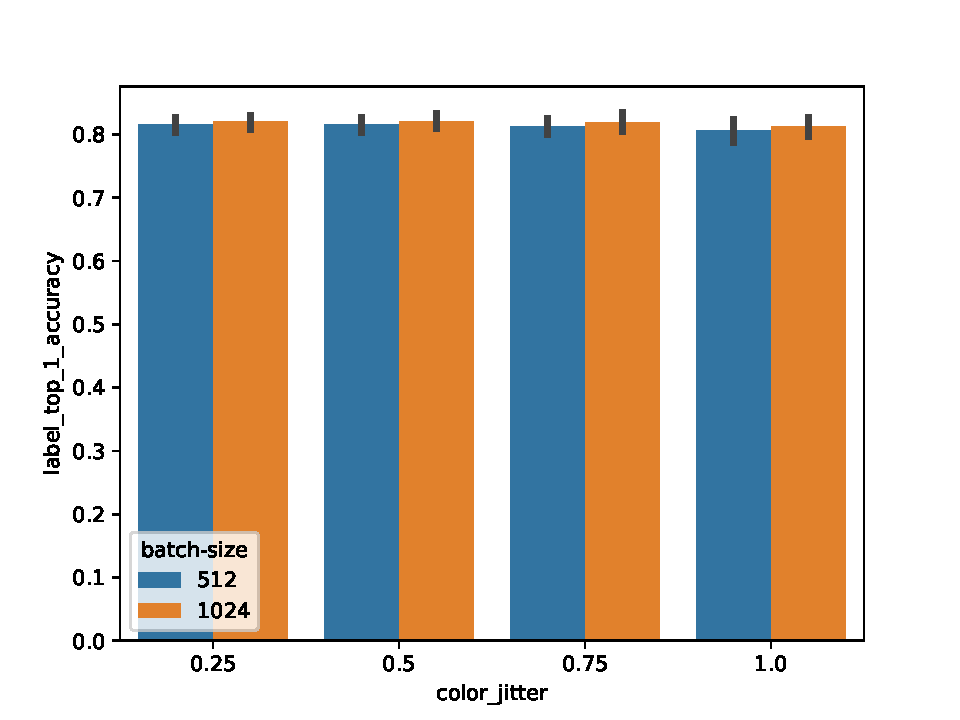
\includegraphics[width=0.55\textwidth]{color-jitter-impact-simclr}%
    
    \label{exp:simclr:colorjitter:impact}
    \caption{Acurracy score following the color jitter parameter and both batch sizes considered.}
\end{figure}

As we can see in Figure \ref{exp:simclr:colorjitter:impact}, the \lstinline{color_jitter_strength} parameter does not have a huge impact on the performance of the linear head of the model. The black bars on the center of each orange/blue bar indicate the variance of the accuracy respect the rest of the parameters. Surely, there are centesimal differences between the different values of this parameter. However, more finetuning might be needed in order to make this parameter relevant for our model. The low influence may as well be caused by the small encoder network (ResNet 18), so we will explore if there are any changes when we change the encoder network later in the document.

\begin{figure}[H] 
    \centering
    \label{exp:simclr:temperature:impact}
        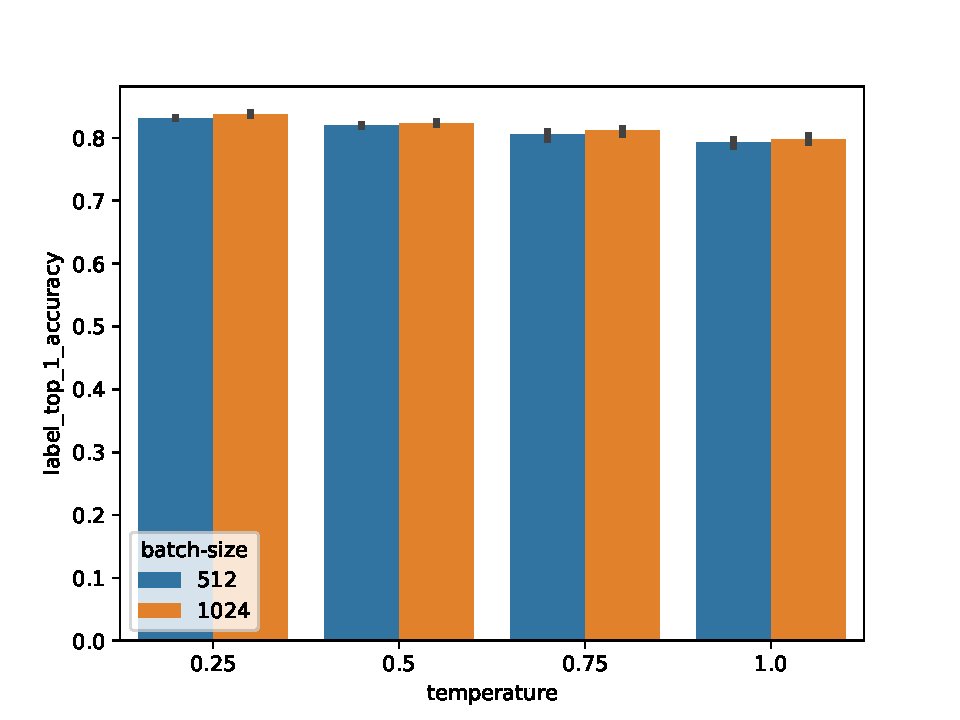
\includegraphics[width=0.55\textwidth]{temperature-impact-simclr}%
       
        \caption{Acurracy score following the temperature and both batch sizes considered.}
\end{figure}


\newpage

\chapter{Conclusions and further work}
In this document, it has been presented an overview of representation learning using contrastive methods. Representation learning is one of the most studied problems in the machine learning field in the last years, so we provided a resume of the first methods that were used, the problems that were found in these methods and how new frameworks emerged to overcome the problems that the first methods were facing.



\newpage 
\
\leavevmode\thispagestyle{empty}\newpage


\chapter*{Acknowledgements}
I would like to thank my tutor, Professor Nicolás Pérez de la Blanca, who has greatly guided me in this work, patiently answering my questions and doubts about the topic.

I would also like to thank my friends for supporting me not only reading this work and providing feedback, but also during the whole bachelor's degree. Specially, thank you to my girlfriend Isabel, who has been my solid ground and has pushed me to be constant and resilient.  

Finally, I would like to thank my family, my very special, weird, but full of love family.

Thank you all. 


\appendix
\renewcommand{\thechapter}{\Alph{chapter}}
\ctparttext{
  \color{red}
  \begin{center}
    Appendices
  \end{center}
}
\part*{Appendix}
\chapter{Appendix A}
\label{APPENDIX:A}

This appendix will be used to set forth some theoretical results that might not always be relevant but are needed to understand some details during this thesis. Not all of them will be proven.

\begin{nprop}[Jensen's Inequality]\label{prop:jensen}
    Let $f:\mathcal D \to \R$ be a concave function and $n\in \mathbb N$. For any $p_1,\dots,p_n \in \R^+_0$ with $\sum p_i = 1$ and any $x_1,\dots,x_n \in \mathcal D$, it holds that:
    $$
    \sum_{i = 1}^n p_i f(x_i) \leq f \left(\sum_{i=1}^n p_i x_i\right).
    $$
    Furthermore, if $f$ is \emph{strictly} concave and $p_i \geq 0$ for all $i  = 1,\dots,n$, then the equality holds if, and only if, $x_1 = \dots = x_n$.
\end{nprop}

In Chapter \ref{Chapter:connection:triplets}, the norm $\norm{\cdot}_2$ is mentioned. Norm theory is a very extense field, so we will only mention the definition and the norm that we will use in the text.

\begin{ndef}\label{def:norm}
Given a vector space $X$ over a subfield $F$ of the complex numbers $\mathbb C$, a \emph{norm} is a real valued function $\norm{\cdot}:X \to \R$ with the following properties:
\begin{enumerate}
\item Triangle inequality, that is: $\norm{x+y} \leq \norm{x} + \norm{y}$ for all $x,y \in X$.
\item Absolute homogeinity, that is: $\norm{sx} = \abs{s}\norm{x}$ for all $x\in X$ and any scalar $s$.
\item Positive definiteness, that is $\norm{x} \geq 0 $ for all $x \in X$ and $\norm{x} = 0$ if, and only if, $x = 0$.
\end{enumerate}
\end{ndef}
In particular, the $\norm{\cdot}_2$ that we used in the euclidean space $\R^n$, is defined as follows:
\[
\norm{x}_2 := \left(\sum_{i = 1}^n x_i^2\right)^{\frac{1}{2}}, \quad \quad \forall x \in \R^n.     
\]
\chapter{Planification and estimated costs}
\input{Chapters/Planning-cost}



\nocite{*}
\bibliographystyle{authordate1}
\bibliography{Bibliography}

\end{document}
